\documentclass[a4paper,onecolumn,11pt,unpublished]{quantumarticle}
\ifdefined\pdfoutput\pdfoutput=1\fi
\usepackage[utf8]{inputenc}
\usepackage[english]{babel}
\usepackage[T1]{fontenc}
\usepackage{amsmath,amssymb,amsthm}
\usepackage{aliascnt}
\usepackage{mathtools}
\usepackage{bm}
\usepackage{braket}
\usepackage{booktabs}
\usepackage{array}
\usepackage{multirow}
\usepackage{graphicx}
\graphicspath{{A_IEEE_TQE/}{output/pdf/}}
\usepackage{microtype}
\usepackage[numbers,sort&compress]{natbib}
\usepackage{hyperref}
\usepackage[nameinlink,capitalize,noabbrev]{cleveref}
\usepackage{quantikz}
\usetikzlibrary{arrows.meta,shapes.geometric}
\usepackage{algorithm} 
\usepackage{algpseudocode}
\usepackage{float}


\usepackage[breakable]{tcolorbox}
\newif\ifreviewcomments
\reviewcommentsfalse
\newcommand{\reviewnote}[3]{%
  \ifreviewcomments
  \begin{tcolorbox}[colback=blue!2!white,colframe=blue!40!black,
    boxrule=0.4pt,arc=0pt,left=6pt,right=6pt,top=4pt,bottom=4pt,
    before skip=7pt,after skip=7pt,
    title={Review #1: #2},fonttitle=\sffamily\bfseries\small]
  \footnotesize\raggedright #3
  \end{tcolorbox}%
  \fi
}


\allowdisplaybreaks
\usepackage{seqsplit}
\setlength{\emergencystretch}{1em}


\newcommand{\bits}{\{0,1\}}
\newcommand{\R}{\mathbb{R}}
\newcommand{\B}{\mathbb{B}}
\newcommand{\Hsupp}{\mathcal{H}_f}
\newcommand{\Dred}{\mathcal{D}}
\newcommand{\Rkeep}{\mathcal{R}}
\newcommand{\Cthree}{\mathcal{C}_3}
\newcommand{\Pset}{\mathcal{P}}
\newcommand{\Yset}{\mathcal{Y}}
\newcommand{\Gred}{\mathcal{G}}
\newcommand{\PiTerm}{\boldsymbol{\Pi}}
\newcommand{\onevec}[1]{\bm{1}_{#1}}
\newcommand{\norminf}[1]{\left\lVert #1\right\rVert_{\infty}}
\newcommand{\PR}{P_{\mathrm R}}
\newcommand{\blankcontent}{\noindent\mbox{}\par}
\DeclareMathOperator*{\argmin}{arg\,min}
\DeclareMathOperator{\msupp}{msupp}
\DeclareMathOperator{\supp}{supp}
\DeclareMathOperator{\diag}{diag}

\newtheorem{definition}{Definition}[section]

\newaliascnt{theorem}{definition}
\newtheorem{theorem}[theorem]{Theorem}
\aliascntresetthe{theorem}

\newaliascnt{lemma}{definition}
\newtheorem{lemma}[lemma]{Lemma}
\aliascntresetthe{lemma}

\newaliascnt{proposition}{definition}
\newtheorem{proposition}[proposition]{Proposition}
\aliascntresetthe{proposition}

\newaliascnt{corollary}{definition}
\newtheorem{corollary}[corollary]{Corollary}
\aliascntresetthe{corollary}

\theoremstyle{remark}
\newaliascnt{remark}{definition}
\newtheorem{remark}[remark]{Remark}
\aliascntresetthe{remark}

\newaliascnt{example}{definition}
\newtheorem{example}[example]{Example}
\aliascntresetthe{example}

\newaliascnt{selectionalgorithm}{definition}
\newtheorem{selectionalgorithm}[selectionalgorithm]{Algorithm}
\aliascntresetthe{selectionalgorithm}

\crefname{definition}{Definition}{Definitions}
\Crefname{definition}{Definition}{Definitions}
\crefname{theorem}{Theorem}{Theorems}
\Crefname{theorem}{Theorem}{Theorems}
\crefname{lemma}{Lemma}{Lemmas}
\Crefname{lemma}{Lemma}{Lemmas}
\crefname{proposition}{Proposition}{Propositions}
\Crefname{proposition}{Proposition}{Propositions}
\crefname{corollary}{Corollary}{Corollaries}
\Crefname{corollary}{Corollary}{Corollaries}
\crefname{example}{Example}{Examples}
\Crefname{example}{Example}{Examples}
\crefname{selectionalgorithm}{Algorithm}{Algorithms}
\Crefname{selectionalgorithm}{Algorithm}{Algorithms}



\title{Exact representation selection and resource trade-offs for quantum optimisation}

\author{Jingcong Liu}
\affiliation{Department of Mathematics, University of Warwick, Coventry CV4 7AL, United Kingdom}
\email{Tom.Liu@warwick.ac.uk}

\author{Yiding Su}
\affiliation{Department of Mathematics, University of Warwick, Coventry CV4 7AL, United Kingdom}
\email{Yiding.Su@warwick.ac.uk}

\author{Ruojun Zhang}   
\affiliation{School of Electronics and Computer Science, University of Southampton, Southampton SO17 1BJ, United Kingdom}
\email{rz4g25@soton.ac.uk}
\usepackage{placeins}
% Keep float-only pages compact; figure PDFs have already been tightly cropped.
\makeatletter
\setlength{\@fptop}{0pt}
\setlength{\@fpsep}{14pt plus 2pt minus 2pt}
\setlength{\@fpbot}{0pt plus 1fil}
\makeatother

\begin{document}
\maketitle

\begin{abstract}
Native higher-order encodings and complete quadratization are two endpoints of an exact representation family with competing resource requirements. We study the selection of executable mixed-locality representations, without assuming an improvement in QAOA solution quality. Direct semantic pair substitutions give a reduction capacity $K_Q$ under auxiliary, penalty and degree budgets. We prove an exact feasibility criterion, derive a closed form for unit-weight pair-star forests, and construct infinitely many instances for which every feasible representation is strictly mixed. An additional corollary establishes simultaneous gate, depth and width separation under an explicitly fixed phase-gadget synthesis. Aggregate-residual penalties and sequential composition provide the underlying pointwise-exactness guarantees. A new 90-instance compilation study finds certified mixed-only budget regions on equal-capacity sparse topologies, while showing that their prevalence and representation rankings depend on synthesis. A separate 60-instance noiseless QAOA study separates classical preparation from incremental evolution; native encoding retains the best mean objective under both equal-effort and scan-refined comparisons. Our contribution is a resource-constrained representation problem, provable phase boundaries within a declared grammar, and reproducible evidence of the limits of compiled and variational advantages.
\end{abstract}

\noindent\textbf{Keywords:} quantum approximate optimisation algorithm; selective locality reduction; pseudo-Boolean optimisation; quadratization; resource-aware quantum algorithms; quantum circuit compilation; warm-start QAOA.

 
\section{Introduction}
\label{sec:introduction}

Higher-order binary interactions arise naturally in clause penalties,
hypergraph objectives and many-body spin models~\cite{BorosHammer2002,Hadfield2021}.
These problems can be written as pseudo-Boolean optimisation,
\begin{equation}
\min_{x\in\{0,1\}^{n}}f(x),\qquad
f(x)=\sum_{A\subseteq[n]}c_A\prod_{i\in A}x_i.
\label{eq:intro-pbo}
\end{equation}
The quantum approximate optimisation algorithm (QAOA) encodes this objective
in a diagonal cost Hamiltonian and alternates cost evolution with mixing
operations~\cite{Farhi2014,Zhou2020}. The mathematical objective, however, does
not specify a unique quantum implementation. Algebraically equivalent
representations can require different registers, interaction graphs, penalty
scales and compiled circuits. Representation is therefore an algorithmic
design choice, especially when qubit capacity, connectivity and executable
depth are simultaneously limited.

Two endpoint strategies dominate current treatments. The first retains the
higher-order objective and directly synthesises its cost evolution. This
native route avoids auxiliary qubits and artificial penalties, and several
comparisons with quadratic encodings report advantages on particular problem
families~\cite{Glos2022,CampbellDahl2022,Stein2023,Bell2025}. Higher-order
phases can be decomposed into one- and two-qubit gates, with circuit-level
optimisation reducing the resulting overhead~\cite{Verchere2023}. Yet a compact
logical register need not give a compact physical circuit: the compiled cost
depends on interaction supports, synthesis and hardware connectivity, and
routing can dominate QAOA implementations on sparse devices
~\cite{Weidenfeller2022,Harrigan2021}.

The second strategy is exact quadratization: construct a quadratic function
$F(x,y)$ whose minimisation over auxiliary variables satisfies
$f(x)=\min_yF(x,y)$ for every original assignment
$x$~\cite{Rosenberg1975,BorosGruber2014,Dattani2019}. Rosenberg substitutions
replace a product such as $x_i x_j$ by an auxiliary bit and add a penalty
enforcing its intended value. This makes pairwise interactions sufficient
at the Hamiltonian level, at the cost of additional qubits and couplings.
The pointwise identity preserves every conditional objective value and the
projected classical minimisers. Complete quadratization can lower logical
locality and simplify individual phase gadgets, but it enlarges the register,
adds couplings and increases coefficient scales. It also changes the spectrum
away from the consistent auxiliary fibres. Consequently, classical exactness
does not imply equal finite-depth QAOA dynamics.

Research on quadratization has substantially improved these endpoint
constructions.
Graph-cut reductions establish useful transformations for higher-order binary
energies~\cite{FreedmanDrineas2005,Ishikawa2011}; general auxiliary-variable
bounds and compact constructions identify what can be achieved for broad
and structured function classes~\cite{AnthonyEtAl2017,Anthony2016,
BorosCramaRodriguezHeck2020}. Optimised and heuristic product substitutions
reduce the auxiliary requirements of higher-degree
objectives~\cite{VermaLewis2020,VermaLewisKochenberger2021}. Recursive
reformulations further connect monomial decomposition, consistency penalties
and convexification~\cite{CramaEtAl2025}. These results establish both the
validity of degree reduction and the importance of the chosen decomposition.

More recent work explicitly addresses their quantum implementation.
Herrman et al. optimise depth in reductions for constrained
problems~\cite{Herrman2021}; Schmidbauer et al. analyse how polynomial
reductions affect QAOA circuits and develop efficient automatic
quadratization for quantum toolchains~\cite{Schmidbauer2024,Schmidbauer2026}.
Rovara et al. select auxiliaries to produce regular interaction graphs with
bounded maximum degree, improving mapping to devices with limited
connectivity~\cite{Rovara2026}. Approximate quadratization instead modifies the
implemented Hamiltonian to reduce circuit cost, accepting a controlled loss of
objective fidelity~\cite{Dragoi2026}. Collectively, these studies establish that
the decomposition matters and that minimising auxiliary count alone is
insufficient. The cited methods address different representation classes and objectives; none should be treated as unable to perform a partial substitution merely because its stated output is quadratic. Table~\ref{tab:related-work-scope} compares their published scope with the narrower question studied here.

\begin{table}[tbp]
\centering\footnotesize
\setlength{\tabcolsep}{3pt}
\renewcommand{\arraystretch}{1.18}
\caption{Scope of representative methods. ``Not studied'' concerns the cited formulation, not impossibility or a claim about every method in that category. The final column refers specifically to a theorem separating native, full and mixed feasibility under joint budgets. Exactness means the pointwise minimum identity, not equality of quantum dynamics.}
\label{tab:related-work-scope}
\begin{tabular}{@{}>{\raggedright\arraybackslash}p{.19\linewidth}>{\raggedright\arraybackslash}p{.10\linewidth}>{\raggedright\arraybackslash}p{.14\linewidth}>{\raggedright\arraybackslash}p{.16\linewidth}>{\raggedright\arraybackslash}p{.15\linewidth}>{\raggedright\arraybackslash}p{.12\linewidth}@{}}
\toprule
Method & Pointwise exact & Mixed output & Joint reduced-set / pair choice & Resource objective & Endpoint phase theorem\\
\midrule
Rosenberg substitution~\cite{Rosenberg1975,BorosGruber2014} & Yes & Partial use possible & Local construction & Not a compiler objective & Not studied\\
Compact quadratization~\cite{BorosCramaRodriguezHeck2020} & Yes & Quadratic output & Construction dependent & Auxiliary bounds & Not studied\\
Automatic full reduction~\cite{Schmidbauer2024,Schmidbauer2026} & Yes & Full-Q target & Substitution choice & Transformation and circuit costs & Not studied\\
Hardware-aware selection~\cite{Rovara2026} & Yes & Full-Q target & Auxiliary selection & Graph structure and mapped depth & Not studied\\
Approximate reduction~\cite{Dragoi2026} & Not in general & Ansatz dependent & Different ansatz space & Qubit and circuit cost & Not studied\\
This work & Yes & Explicit output & Both $\mathcal D$ and $\rho$ & Fixed-compiler joint budgets & Within direct pair grammar\\
\bottomrule
\end{tabular}
\end{table}

A digital processor can execute a mixed-locality Hamiltonian: a limited number of auxiliaries may replace expensive interactions while other terms remain native. Partial use of an exact substitution is a natural option, and the Rosenberg gadget itself is not our novelty claim. The question is when the freedom to select both reduced terms and their shared pairs is necessary for resource feasibility. We answer it within a declared direct-pair grammar, rather than asserting that mixed representations are universally superior or unavailable to other frameworks.

Making this intermediate space rigorous is not a matter of independently
replacing convenient monomials. When several selected terms share an
auxiliary, the penalty must dominate their aggregate residual rather than each
coefficient in isolation. Successive substitutions may themselves involve
earlier auxiliaries, so exactness must survive composition. Finally, a useful
selection rule must compare the qubits saved or spent against compiled gate
count, depth, connectivity and penalty scale. These requirements define the
central problem addressed here: how can one select a partially reduced
representation while preserving the original objective pointwise and making
its resource guarantees explicit?

Initialisation introduces a further representation dependence.
Relaxation-based warm starts use classical optimisation information to
construct an initial quantum state and a compatible
mixer~\cite{Egger2021}; semidefinite initialisation and custom mixers have
further developed this approach~\cite{TateSDP2023,TateCustom2023}.
When a reformulation adds a variable representing $x_i x_j$, however, its
initial marginal must also be specified. A pair pseudo-moment from a
relaxation can differ from the product of its single-variable marginals.
This creates a concrete choice about how to initialise the enlarged
register, while neither choice alone enforces the auxiliary relation in a
product state. A selective framework must therefore connect representation
choice to an initialisation policy without conflating classical exactness,
initial fibre consistency and subsequent QAOA performance.

Our principal theoretical contribution is a resource-feasibility result. A capacity $K_Q$ characterises how many cubic terms can be reduced under simultaneous auxiliary, penalty and auxiliary-degree limits. For pair-star forests we compute this capacity in closed form and obtain explicit phase boundaries, including an infinite family in which both endpoints fail but a mixed representation is feasible. A separate corollary counts emitted gates and scheduled two-qubit depth under a fixed phase-gadget synthesis. The static theorem does not depend on a compiler; the compiled corollary does.

The exactness machinery supports this representation problem. We state the sharp aggregate-residual Rosenberg threshold and its compositional extension to arbitrary degree. These are guarantees for a specified construction, not universal minimum penalties over all reformulations. At higher degree the sharp residual norm may itself require difficult Boolean optimisation; a coefficient-sum bound remains an efficiently computable sufficient alternative. Practical selection and small exact certificates are distinguished from a claim of scalable global search.

Experimentally, the main comparison is between minimising the same resource score over full reductions and over the larger selective family. Compiled joint-budget maps assess executable representations; warm-state controls and larger optimisation budgets assess a separate question about solution quality. The original 14-instance QAOA comparison, 20-instance signal-enriched study and 18-instance noise study are development evidence throughout. In particular, the native mean values in Table~\ref{tab:e3-qaoa-summary} are an important boundary result. Neither pointwise exactness nor smaller circuits establishes a QAOA performance advantage, and a distinct advantage from auxiliary pair moments remains unresolved.

\section{Results}
\label{sec:results}

We first establish the exact representation family and then compare its
members through compilation and QAOA experiments. The algebraic guarantees
hold independently of the benchmark data; the resource and optimisation
conclusions concern the evaluated instances and protocols.

\subsection{Representation framework}
\label{sec:preliminaries}
\label{sec:pb-diagonal}
\label{sec:pointwise-exactness}
\label{sec:resource-relaxation-data}

\begin{table}[htbp]
\centering
\caption{Core notation. Subscripts $\sigma$ indicate dependence on the chosen representation.}
\label{tab:notation}
\small
\renewcommand{\arraystretch}{1.08}
\begin{tabular}{@{}p{0.25\linewidth}p{0.71\linewidth}@{}}
\toprule
Symbol & Meaning \\
\midrule
$\mathbb B$, $[n]$ & $\{0,1\}$ and $\{1,\ldots,n\}$. \\
$x$, $y$, $u=(x,y)$ & Original bits, auxiliary bits, and the combined register. \\
$x_A$, $c_A$ & $\prod_{i\in A}x_i$ and its coefficient in $f$; $x_\varnothing=1$. \\
$f$, $F_\sigma$ & Original objective and its pointwise-exact representation. \\
$\sigma$, $a_\sigma$, $N_\sigma$ & Representation choice, auxiliary count, and total qubits $n+a_\sigma$. \\
$\ell$, $L_\sigma$ & Target locality of reduced terms and maximum retained locality. \\
$\mathcal D$, $\mathcal R$ & Higher-order terms chosen for reduction and those retained. \\
$p$, $y_p$, $P_\rho$ & A variable pair, its product auxiliary, and the active pair set. \\
$M_p$, $T_p$, $M_{\max,\sigma}$ & Pair penalty, its exactness threshold, and largest active penalty. \\
$\mathcal Y_F(x)$ & Auxiliary assignments minimising $F(x,\cdot)$. \\
$H_F$, $Z_i$ & Diagonal cost Hamiltonian and the Pauli $Z$ operator on qubit $i$. \\
$G_{2q,\sigma}$, $D_{2q,\sigma}$, $S_\sigma$ & Compiled two-qubit gate count, two-qubit depth, and SWAP count. \\
$\kappa_\sigma$ & Largest-to-smallest magnitude ratio of nonzero, nonidentity Pauli coefficients. \\
$\bar\mu_i$, $\bar q_{ij}$ & Raw single and pair pseudo-moments from a common relaxation. \\
$\mu_i$, $q_p$ & Preparation probabilities from clipped moments or the stated independence fallback. \\
\bottomrule
\end{tabular}
\par\smallskip
\begin{minipage}{\linewidth}\footnotesize
In the constructions, $p$ denotes a variable pair; in experimental tables
and figures it denotes QAOA depth (written $r$ in the ansatz).
\end{minipage}
\end{table}

Let $\mathbb B=\{0,1\}$ and $x_A=\prod_{i\in A}x_i$, with
$x_\varnothing=1$. The objective in Eq.~\eqref{eq:intro-pbo} has diagonal
encoding
\begin{equation}
H_f=f(N_1,\ldots,N_n),\qquad N_i=(I-Z_i)/2,\qquad
H_f|x\rangle=f(x)|x\rangle.
\label{eq:diagonal-cost}
\end{equation}
Its nonconstant logical locality is $\deg(f)$~\cite{Hadfield2021}.
A representation $F_\sigma$ with $a_\sigma$ auxiliary bits is pointwise exact
when
\begin{equation}
f(x)=\min_{y\in\mathbb B^{a_\sigma}}F_\sigma(x,y)
\qquad\text{for every }x\in\mathbb B^n.
\label{eq:pointwise-exactness}
\end{equation}
This preserves the optimum and projected minimisers, while leaving the
Hamiltonian spectrum outside the optimal auxiliary fibres unconstrained.
The construction uses the Rosenberg penalty~\cite{Rosenberg1975}
\begin{equation}
P_{\mathrm R}(a,b,y)=ab-2ay-2by+3y,
\qquad P_{\mathrm R}=0\text{ if }y=ab,
\quad P_{\mathrm R}\geq1\text{ otherwise}.
\label{eq:rosenberg}
\end{equation}

Table~\ref{tab:notation} distinguishes representation resources from
relaxation data. Raw pseudo-moments need not describe a joint probability
law. They define the selector diagnostic, while state preparation uses
clipping or the specified independence fallback. Detailed identities and
resource definitions are in Appendix~\ref{app:background-details}.

\subsection{Exact selective locality reduction}
\label{sec:cubic-quadratization}
\label{sec:one-step-substitution}
\label{sec:compositional-exactness}

For a collected multilinear polynomial $q(u)=\sum_S d_Su_S$ on
$\mathbb B^N$, choose a pair $p=\{i,j\}$ and a family
$\mathcal S_p$ of higher-order terms containing it. Collect the selected
residual as $A_p(v)=\sum_{S\in\mathcal S_p}d_Su_{S\setminus p}$, where
$v$ omits $u_i,u_j$, and write
\begin{equation}
q(u)=B_p(u)+u_i u_jA_p(v).
\label{eq:aggregate-residual-decomposition}
\end{equation}
Replacing the shared product by one fresh auxiliary gives
\begin{equation}
Q_{p,M_p}(u,y_p)=B_p(u)+y_pA_p(v)+M_pP_{\mathrm R}(u_i,u_j,y_p).
\label{eq:one-step-reformulation}
\end{equation}
The Rosenberg construction is standard~\cite{Rosenberg1975,BorosGruber2014};
the relevant penalty must control the aggregate of all terms sharing $y_p$.

\begin{proposition}[Sharp aggregate-residual penalty]
\label{prop:sharp-aggregate-residual}
For $M_p\geq0$, with $\|A_p\|_\infty:=\max_{v\in\mathbb B^{N-2}}|A_p(v)|$,
\begin{equation}
q(u)=\min_{y_p\in\mathbb B}Q_{p,M_p}(u,y_p)\quad\text{for every }u
\quad\Longleftrightarrow\quad M_p\geq\|A_p\|_\infty.
\label{eq:sharp-one-step-threshold}
\end{equation}
The consistent value $y_p=u_i u_j$ is the unique minimiser for every $u$
if and only if $M_p>\|A_p\|_\infty$.
\end{proposition}

An inconsistent value changes the selected block by at most
$\|A_p\|_\infty$ and incurs a penalty of at least $M_p$.
Appendix~\ref{app:sharp-one-step-proof} proves sharpness and the separation
margin. For successive substitutions, compute each residual from the
\emph{current} polynomial, treating earlier auxiliaries as independent
Boolean coordinates.

\begin{theorem}[Sequential compositional exactness]
\label{thm:sequential-compositional-exactness}
Let $g^{(0)}=f$, and form $g^{(r)}$ from $g^{(r-1)}$ by
Eq.~\eqref{eq:one-step-reformulation} using a fresh $y_r$ and
$M_r\geq\|A_r\|_\infty$. Then the recursively consistent lift $\Phi(x)$ satisfies
\begin{equation}
f(x)=\min_{y\in\mathbb B^R}g^{(R)}(x,y)=g^{(R)}(x,\Phi(x)).
\label{eq:compositional-exactness}
\end{equation}
If every inequality is strict, $\Phi(x)$ is the unique auxiliary minimiser.
\end{theorem}

The threshold is sharp only within the chosen Rosenberg substitution.
For arbitrary degree, computing $\|A_p\|_\infty$ can require exponential
Boolean optimisation. The bound $M_p\geq\sum_{S\in\mathcal S_p}|d_S|$
is sufficient and easy to compute, but need not be sharp.
The one-step inequalities telescope; the full gap bound and proof are in
Appendix~\ref{app:compositional-proof}. Consequently, any selected degree-$k$
term can be reduced to target locality $\ell\geq2$ with at most
$\max\{k-\ell,0\}$ fresh auxiliaries. Unselected terms remain native.
Corollary~\ref{cor:selective-target-locality} gives the construction and total
bound. Sharing intermediate products can save auxiliaries, but requires
recomputing their aggregate penalties.

\subsection{The cubic design space}
\label{sec:cubic-specialisation}

The main empirical studies use cubic objectives
$f=f_{\leq2}+\sum_{A\in\mathcal C_3(f)}c_Ax_A$, where
$\mathcal C_3(f)=\{A\subseteq[n]:|A|=3,\ c_A\neq0\}$.
A design $\sigma=(\mathcal D,\rho)$ chooses the reduced supports
$\mathcal D\subseteq\mathcal C_3(f)$ and a pair
$\rho(A)\in\binom A2$ for each $A\in\mathcal D$.
Write $\mathcal R=\mathcal C_3(f)\setminus\mathcal D$,
$P_\rho=\rho(\mathcal D)$ and
$\mathcal D_p=\{A\in\mathcal D:\rho(A)=p\}$.
With $A_p(x)=\sum_{A\in\mathcal D_p}c_Ax_{A\setminus p}$,
\begin{equation}
F_{\rho,M}(x,y)=f_{\leq2}(x)+\sum_{A\in\mathcal R}c_Ax_A
+\sum_{p\in P_\rho}y_pA_p(x)
+\sum_{p=\{i,j\}\in P_\rho}M_pP_{\mathrm R}(x_i,x_j,y_p).
\label{eq:cubic-mixed-objective}
\end{equation}
Each $A_p$ is linear in distinct remaining coordinates, so
\begin{equation}
C_p^+=\sum_{A\in\mathcal D_p,\,c_A>0}c_A,\qquad
C_p^-=\sum_{A\in\mathcal D_p,\,c_A<0}|c_A|,\qquad
T_p:=\max\{C_p^+,C_p^-\}=\|A_p\|_\infty.
\label{eq:cubic-threshold}
\end{equation}

\begin{proposition}[Exact cubic mixed-sign reduction]
\label{prop:cubic-mixed-sign}
For nonnegative penalties, $f(x)=\min_yF_{\rho,M}(x,y)$ for every $x$
if and only if $M_p\geq T_p$ for every active pair. Strict inequalities give
the unique lift $\phi_\rho(x)=(x_ix_j)_{p=\{i,j\}\in P_\rho}$.
\end{proposition}

Minimisation separates over auxiliaries, so the claim follows from
Proposition~\ref{prop:sharp-aggregate-residual}. Fixing positive margins gives
the finite exact family $\Sigma_{\mathrm{ex}}^\varepsilon$ through
\begin{equation}
M_p=T_p+\varepsilon_p,\qquad \varepsilon_p>0\text{ fixed}.
\label{eq:canonical-cubic-penalty}
\end{equation}
Its endpoints are the native design ($\mathcal D=\varnothing$) and fully
reduced designs ($\mathcal D=\mathcal C_3(f)$); intermediate choices retain
mixed locality. The auxiliary count is $a_\sigma=|P_\rho|$, rather than
the number of reduced terms. Appendix~\ref{app:cubic-structure} characterises
this reuse by pair cover.




% Insert after the cubic exactness construction. This file is a drafting
% artifact; paste into main.tex, rather than modifying other manuscript files.
\section{When resources force a mixed representation}
\label{sec:representation-phases}

Pointwise exactness does not imply equal QAOA dynamics or solution quality.
It does, however, permit a precise feasibility question before optimisation:
can any exact representation meet the simultaneous resource budgets?
The results in this section concern the direct cubic pair grammar of
Eq.~\eqref{eq:canonical-cubic-penalty}; they do not assert impossibility for
arbitrary quadratizations, coefficient splitting, or cross-auxiliary penalties.

\subsection{Static capacity and exact phase boundaries}
Let $E=\mathcal C_3$, $m=|E|$, and $\sigma=(\mathcal D,\rho)$.
For an active pair $p$, write $q_p=|\mathcal D_p|$ and
$T_p=\max\{\sum_{A\in\mathcal D_p:c_A>0}c_A,
\sum_{A\in\mathcal D_p:c_A<0}|c_A|\}$.
Fix a uniform margin $\varepsilon\geq0$ and use
$M_p=T_p+\varepsilon$. At $\varepsilon=0$ the representation is value-exact,
but an inconsistent auxiliary may tie; $\varepsilon>0$ gives the unique
consistent minimising lift. In particular, an actual penalty budget bounds
$T_p+\varepsilon$, not just $T_p$.
The static resource vector is
\[
 \left(|P_\rho|,\;\max_{p\in P_\rho}(T_p+\varepsilon),\;
 \max_{p\in P_\rho}(q_p+2),\;|E\setminus\mathcal D|\right),
\]
where maxima over the empty set are zero. The auxiliary degree is exactly
$q_p+2$ in the interaction support of this direct cubic construction.
For budgets $(r_0,M_0,\Delta_0,h_0)$, with $r_0,h_0$ nonnegative integers,
let $\mathcal Q(r_0,M_0,\Delta_0)$ contain the subsets $\mathcal D$
admitting an assignment satisfying the first three budgets, and define
\begin{equation}
 K_Q(E,c;r_0,M_0,\Delta_0)
 =\max_{\mathcal D\in\mathcal Q(r_0,M_0,\Delta_0)}|\mathcal D|.
 \label{eq:static-reduction-capacity}
\end{equation}
Restricting an assignment to a subset cannot increase the number of active
pairs, either signed coefficient sum, or auxiliary degree. Thus
$\mathcal Q$ is downward closed.

\begin{theorem}[Exact static feasibility boundary]
\label{thm:static-phase-boundary}
A feasible direct-pair representation exists if and only if $K_Q+h_0\geq m$.
The native endpoint is feasible if and only if $h_0\geq m$; a fully reduced
representation is feasible if and only if $K_Q=m$. Consequently, feasible
representations exist and all are strictly mixed exactly when
\begin{equation}
 K_Q<m,\qquad h_0<m,\qquad K_Q+h_0\geq m.
 \label{eq:static-mixed-only}
\end{equation}
\end{theorem}
\begin{proof}
Every feasible design reduces at least $m-h_0$ terms, giving necessity.
Conversely, a capacity-achieving reduced set leaves $m-K_Q\leq h_0$ native
terms. The endpoint criteria follow from their definitions.
\end{proof}

A \emph{pair-star} with $\ell$ petals has supports
$\{\{a,b,w_t\}:1\leq t\leq\ell\}$, with all vertices distinct apart from
the core $\{a,b\}$. A pair-star forest is a vertex-disjoint union of such
stars; a one-petal star is an isolated triple.

\begin{theorem}[Closed form for a unit-weight pair-star forest]
\label{thm:pair-star-capacity}
Suppose all cubic coefficients are $+1$ and the star sizes are
$\ell_1,\ldots,\ell_s\geq1$. Put $m=\sum_i\ell_i$ and
\[
 C=\max\{0,\min\{\lfloor M_0-\varepsilon\rfloor,
                         \lfloor\Delta_0\rfloor-2\}\}.
\]
If $r_0=0$ or $C=0$, then $K_Q=0$. Otherwise, let
$g_i=\min\{\ell_i,C\}-1$, sort these gains in nonincreasing order,
and set $\rho_0=\min\{r_0,s\}$. Then
\begin{equation}
 K_Q=\min\left\{m,\;r_0+\sum_{j=1}^{\rho_0}g_{(j)}\right\}.
 \label{eq:pair-star-capacity}
\end{equation}
\end{theorem}
\begin{proof}
A bucket of $q$ unit terms has $T_p=q$ and degree $q+2$, so its capacity is
$C$. Only a star's core pair can be shared by distinct petals. If $r$ pairs
are active and the selected cores are indexed by $I$, at most
$r+\sum_{i\in I}g_i$ terms are reduced. This proves the upper bound.
For attainment, select the $\rho_0$ highest-gain cores and fill their buckets
to $\min\{\ell_i,C\}$. Spend each remaining auxiliary on a distinct private
pair of an uncovered petal until the budget or the support is exhausted.
This attains the stated minimum, including when the gains vanish.
\end{proof}

Write $R_Q=r_0+\sum_{j=1}^{\rho_0}g_{(j)}$, with $R_Q=0$ if $r_0=0$ or
$C=0$. The following boundaries are therefore exact within the stated grammar.
Here ``native only'' and ``full-Q only'' describe endpoint feasibility;
mixed designs can also be feasible in those rows.
\begin{center}
\begin{tabular}{ll}
\toprule
Feasibility class & Necessary and sufficient condition\\
\midrule
Both endpoints & $R_Q\geq m,\ h_0\geq m$\\
Native endpoint only & $R_Q<m,\ h_0\geq m$\\
Full-Q endpoint only & $R_Q\geq m,\ h_0<m$\\
Mixed only & $R_Q<m,\ h_0<m,\ R_Q+h_0\geq m$\\
None & $R_Q+h_0<m$\\
\bottomrule
\end{tabular}
\end{center}

\begin{corollary}[An infinite static mixed-only family]
\label{cor:static-star-isolated}
For every $L,H\geq1$, take the disjoint union of an $L$-petal unit pair-star
and $H$ unit isolated triples. Under budgets
$(r_0,M_0,\Delta_0,h_0)=(1,L+\varepsilon,L+2,H)$,
neither endpoint is feasible, whereas reducing the star through its core
and retaining all isolated triples is feasible.
\end{corollary}
\begin{proof}
The stated design has exactly that resource vector. The native endpoint
retains $L+H>H$ cubic terms. Every full reduction needs at least one pair
for the star and a distinct pair for each isolated triple, hence at least
$H+1>1$ auxiliaries, irrespective of its pair-assignment heuristic.
\end{proof}

The endpoints are also incomparable under a common budget. For any
$h\geq2$, use $(r_0,M_0,\Delta_0,h_0)=(1,h+1+\varepsilon,h+3,h)$.
The union of $h$ isolated unit triples admits its native endpoint but no
full reduction. A unit pair-star with $h+1$ petals admits a full reduction
through its core but not its native endpoint. Thus locality alone does not
order feasibility.

\subsection{A compiled-resource consequence under a fixed synthesis}
\label{sec:compiled-phase-corollary}
Static feasibility alone is not a gate or depth theorem. To connect the two,
fix the reference synthesis $\Pi$ of
Appendix~\ref{app:reference-compiler}: collect equal Pauli strings after
$x_i=(1-Z_i)/2$, drop exact zeros, use a symbolic cost angle, order strings
by weight and lexicographic support, implement each string by a parity
gadget onto its largest-index qubit, and schedule the resulting CNOT stream
by the stated earliest-layer rule. There is all-to-all connectivity and no
cross-gadget cancellation in this particular theorem. $G_{2q}^\Pi$ and
$D_{2q}^\Pi$ count CNOTs and their depth for one cost layer, excluding
single-qubit gate durations. These are realised circuit costs under $\Pi$,
not lower bounds on all possible synthesis procedures.

\begin{corollary}[An infinite compiled mixed-only family under $\Pi$]
\label{cor:compiled-star-isolated}
Let $L\geq2$, $H\geq1$, and $\varepsilon>0$. On
$n=L+2+3H$ original bits consider
\[
 f_{L,H}(x)=x_ax_b\sum_{t=1}^{L}x_{w_t}
              +\sum_{j=1}^{H}x_{u_j}x_{v_j}x_{z_j}.
\]
Order the original variables as $a,b,w_1,\ldots,w_L$, followed by each
isolated triple in order, and append auxiliaries in pair order.
Use $M_p=T_p+\varepsilon$ and budgets
\begin{equation}
 Q_{\max}=n+1,\qquad G_{\max}=2L+6+10H,\qquad
 D_{\max}=2L+6,\qquad M_{\max}=L+\varepsilon.
 \label{eq:compiled-mixed-only-budgets}
\end{equation}
The native circuit violates both the gate and depth budgets; every fully
reduced direct-pair representation violates the width budget. Reducing only
the star through its core meets all four budgets and is pointwise exact
with a unique consistent minimising lift.
\end{corollary}
\begin{proof}
After collection, the native star contains $2L+1$ nonzero weight-two strings
and $L$ nonzero weight-three strings. The reduced star contains $L+3$
nonzero weight-two strings and no weight-three strings: its quadratic
supports are $\{a,b\}$, $\{a,y\}$, $\{b,y\}$, and
$\{w_t,y\}$ for $1\leq t\leq L$. Their coefficients do not cancel for
$M=L+\varepsilon>0$. Each isolated native triple contributes three
weight-two and one weight-three string. Since $\Pi$ uses $2(k-1)$ CNOTs
for a weight-$k$ string, the respective gate counts are
\[
 G_{2q}^{\Pi,\mathrm{native}}=8L+2+10H,
 \qquad G_{2q}^{\Pi,\mathrm{mixed}}=2L+6+10H.
\]
For depth, the native star's ordered pair gadgets finish with the core
qubits at layers $2L+2$ and $2L+4$. Its first triple gadget ends at layer
$2L+7$ when $L\geq2$; every remaining triple adds four layers.
Hence its depth is $6L+3$. In the reduced star, the core pair is followed
by the two core--auxiliary pairs and then the $L$ leaf--auxiliary pairs,
giving depth $2L+6$. An isolated native triple has depth $10$ and runs on
disjoint wires. Consequently
\[
 D_{2q}^{\Pi,\mathrm{native}}=6L+3,
 \qquad D_{2q}^{\Pi,\mathrm{mixed}}=\max\{2L+6,10\}=2L+6.
\]
The gate difference $6L-4$ and depth difference $4L-3$ are positive.
The mixed design uses one auxiliary and penalty $L+\varepsilon$.
Every full reduction uses at least $H+1$ auxiliaries by
Corollary~\ref{cor:static-star-isolated}, proving the width obstruction.
\end{proof}

This is a feasibility result for a specified compilation model and a
specified family, not a statement about QAOA solution quality. Its endpoint
obstruction covers all full reductions in the declared grammar, rather
than merely a selected baseline. Optimised gadget orderings, cancellation,
and routed topologies define different compilers and require fresh resource
measurements; the empirical tests below address that separate question.
Arbitrary affine terms may be added to $f_{L,H}$ without changing this
corollary: they change the objective landscape but introduce no two-qubit
Pauli supports.


\section{Resource and QAOA evaluation}
\label{sec:new-evaluation}
% Suggested prose to integrate into main.tex, not a replacement manuscript.
\subsection{Fresh joint-budget compilation study}
\label{sec:fresh-compiled}

The new experiment asks whether a strictly mixed representation can be the
only executable member of the direct-pair representation family under joint
budgets. This is distinct from asking which unconstrained representation
minimises a weighted resource score, and from asking which gives the best
QAOA objective value. We froze the implementation, generators, candidate
budgets, resource weights, compiler settings and budget grid before generating
30 new Max3SAT and 30 new cubic-spin instances. These small instances have
six variables and five distinct cubic supports. Max3SAT signs and spin
coupling signs are sampled independently; the latter objectives are divided
by eight after conversion to Boolean variables. They are a new, explicitly
specified distribution, rather than an extension of the old instance pool.

We additionally generated 30 nine-variable, four-leaf pair-star-plus-isolated
instances, with random vertex labels and independent positive weights in
$\{0.75,1,1.25\}$. This is a mechanism study. Its initial 32-candidate
assertion exposed a structural corner case: only 27 full assignments fit
the 12-qubit device. Before obtaining any constructed-instance compiler
result, we documented an amendment capping both searches at 27 candidates
for this family. All 60 random-instance results retain the original frozen
protocol. The original source, amendment, timestamps and hashes accompany
the data; this local prospective freeze is not an external preregistration.

For each target, both full and mixed search minimise the same objective,
\begin{equation}
 J_{\rm new}=\frac14\left(\frac{a}{4}+\frac{G_{\rm CX}}{160}
                    +\frac{D_{\rm CX}}{120}+\frac{M_{\max}}{8}\right).
 \label{eq:new-compiled-score}
\end{equation}
Each search scores 32 distinct capacity-feasible candidates per random
instance and target, or 27 per constructed instance. Full search requires
$D=E$; mixed search admits all four actions per cubic, including the
endpoints. Both include minimum-auxiliary, maximum-reuse and a simple
distance-aware full assignment. The remaining proposals are drawn once
from a seeded permutation; mixed proposals also include native, common-pair
buckets and reuse prefixes. This finite search does not certify a global
minimum. Sharing identical compiler evaluations does not enlarge either
candidate budget. All $3^5$ full assignments are enumerated logically;
the 27 capacity-feasible full assignments in the constructed family are
also exhaustively compiled.

Minimum-auxiliary full reduction tests whether auxiliary minimisation alone
explains a result; maximum reuse tests reuse alone; resource-optimised full
reduction tests the additional freedom to retain cubic terms under equal
candidate budgets. The distance-aware comparator selects the shortest
original-variable pair and breaks ties by reuse. It is an inspired heuristic,
not an implementation of a named hardware-aware algorithm. A random control
matches both $a$ and $|D|$ of the best strict mixed candidate, and also matches
$M_{\max}$ whenever a distinct exact match exists. This latter match exists
in 495 of 540 instance--target--synthesis settings; 15 settings have no
distinct control with the required $a,|D|$ and are recorded as degenerate.
These repeated settings are not independent experimental units.

All representations use $M_p=1.1\max(C_p^+,C_p^-)$ and symbolic $\gamma$.
Qiskit 2.5.2 compiles the actual aggregated Pauli cost circuits to
$\{\mathrm{CX},R_Z,\mathrm{SX},X\}$ with optimisation level 3, SABRE routing,
identity initial placement and seed 1729. Selection is repeated directly on
line-12, ring-12 and $3\times4$ grid-12. The canonical synthesis uses
size/lexical gadget ordering; reuse synthesis groups commuting gadgets by
a frequent root and greedily orders their parity supports. Neither inserts
gadget barriers, allowing optimisation across gadget boundaries. This tests
two synthesis strategies within one pinned compiler, not independent compiler
implementations or seed robustness. $G$ is CX count and $D$ is CX-only
scheduled depth, not physical duration. $Q$ counts occupied input sites and
every physical site used during routing; logical width $n+a$ is also saved.
These are cost-layer resources and exclude preparation and mixers.

The frozen grid is
\[
\begin{aligned}
Q_{\max}&\in\{6,\ldots,12\}, & G_{\max}&\in\{0,4,\ldots,240\},\\
D_{\max}&\in\{24,48,72,96,120,160,240\},\\
M_{\max}&\in\{0,1.1,2.2,3.3,4.4,6.6,8.8\}.
\end{aligned}
\]
We classify each cell as both endpoints feasible, native endpoint only,
full endpoint only, strict mixed only, or none found in the candidate
library. Endpoint-only labels can include feasible mixed candidates.
``None found'' is not a global infeasibility certificate. A stricter
certified subset requires native to satisfy width but violate its compiled
gate/depth budget, a compiled mixed candidate to satisfy all budgets, and
exhaustive logical enumeration to exclude every full assignment through
width or penalty. The cell counts are correlated descriptions of a fixed
grid, not independent trials.

\begin{table}[t]
\centering\small
\begin{tabular}{lccc}
\toprule
Family & Line-12 & Ring-12 & Grid-12\\
\midrule
Max3SAT, $N=30$ & $16/8$ & $16/8$ & $18/8$\\
Cubic spin, $N=30$ & $1/0$ & $1/0$ & $1/0$\\
Constructed, $N=30$ & $30/29$ & $30/22$ & $30/28$\\
\bottomrule
\end{tabular}
\caption{Independent instances with at least one certified strict-mixed-only
cell anywhere in the frozen grid. Each entry is canonical/reuse synthesis.
The constructed cohort follows the disclosed technical amendment.}
\label{tab:new-compiled-feasibility}
\end{table}

Across the six compiler settings, 23/30 Max3SAT and 30/30 constructed
instances have a certified strict-mixed-only region in at least one setting;
3/30 and 21/30 respectively have one in every setting. The cubic-spin result
is substantially weaker: only 2/30 have such a region anywhere, and none
does under reuse synthesis. Thus compiled necessity is demonstrable but
neither universal nor synthesis-independent at the instance level.

\begin{figure*}[t]
\centering
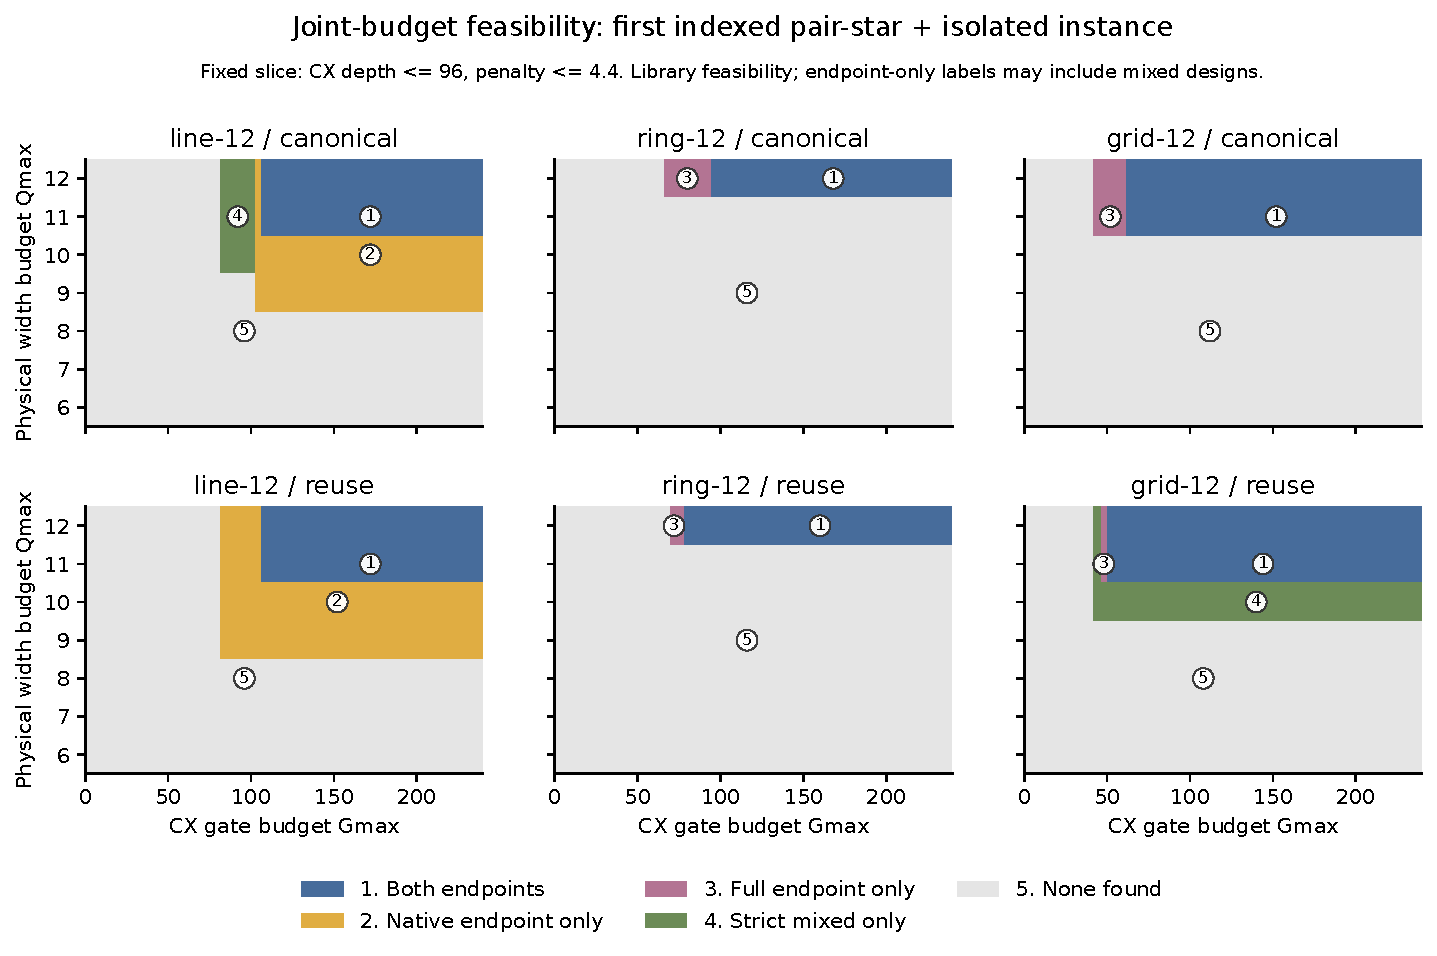
\includegraphics[width=\textwidth]{figures/joint_budget_phase_map.pdf}
\caption{Real-compiler joint-budget phase maps for the first indexed
constructed instance at $D_{\max}=96$, $M_{\max}=4.4$. Width is physical
routing footprint. The same device capacity is used throughout. This is
an illustrative slice; population counts use the complete frozen grid.
The full endpoint is exhaustive over capacity-feasible assignments for
this constructed family; the mixed candidate library remains finite.}
\label{fig:new-joint-phase}
\end{figure*}

A concrete post-hoc explanatory example, chosen within the unchanged
budget grid, uses the first indexed constructed instance on ring-12 with
canonical synthesis. At $(Q_{\max},G_{\max},D_{\max},M_{\max})
=(12,92,48,2.2)$, the measured native resources are $(12,96,55,0)$,
a full candidate has $(12,80,40,3.85)$, and a strict mixed candidate has
$(12,92,43,2.2)$. Native exceeds both cost bounds; the full candidate
passes those bounds but exceeds the penalty bound. More strongly, every
full assignment with logical width at most 12 has $M_{\max}\ge2.475$.
All remaining full assignments exceed width, while the displayed mixed
candidate is feasible. Recompilation reproduces all three resource records.
This example establishes feasibility of an exact representation, not an
improvement in QAOA solution quality.

The best strict mixed candidate has lower $J_{\rm new}$ than the
resource-optimised full candidate on all 90 instances in each of the six
settings. Nevertheless, unrestricted mixed search selects the native
endpoint in every random-instance setting and in 173/180 constructed
settings. The weighted score therefore does not by itself recommend an
intermediate representation: hard joint budgets provide the stronger
reason to use one. The matched random control is also not uniformly worse;
properly matched controls sometimes equal or beat the selected strict
mixed candidate, as expected from a finite search and a single random draw.

Rank stability is incomplete. Across canonical versus reuse synthesis,
median Spearman correlations of $J_{\rm new}$ on common candidate identities
are $0.913,0.915,0.949$ for Max3SAT on line, ring and grid;
$0.906,0.905,0.955$ for cubic spin; and $0.771,0.729,0.812$ for the
constructed family.

Median Pareto-set overlaps in $(Q,G,D,M)$, measured by Jaccard similarity, are $0.333,0.250,0.333$; $1,1,1$; and
$0.321,0.351,0.355$. Full-search winners change in 6--14 of 30 Max3SAT
instances, 10--13 of 30 spin instances, and 0--4 of 30 constructed
instances, depending on topology. Stable aggregate ranks therefore do not
imply stable frontiers or selected assignments. The new evidence consists
of 31,577 compiler calls, with 32,760 scheduled candidate
evaluations before sharing repeated designs, and independently checked
logical and routed-circuit semantics.

\subsection{Fresh evaluation: preparation and incremental evolution}

\label{sec:fresh-qaoa}

To separate preparation from subsequent evolution, we froze the implementation, seeds, hypotheses and budgets locally before generating 30 new independent instances of each family. These are uniform, $n=6$ instances with six clauses or spin interactions, subject only to coverage and at least two nonzero cubic monomials. This scope is deliberately small and noiseless. The earlier 14-instance QAOA set and 20-/18-instance follow-up sets are exploratory; signal-enriched samples are mechanism studies. The new protocol is locally prospective, not an externally registered study.

We compare native, proper mixed ($0<|D|<|E|$), and fully reduced representations. Both reduction domains receive up to 128 distinct seeded candidate evaluations under the same reference-compiler score $J_{\rm res}=(a/4+G/160+D_2/120+M/8)/4$, with exhaustive evaluation if a domain is smaller. These proper-mixed arms are conditional representation comparisons: native has the lowest resource score among all evaluated candidates on all 60 instances. Penalties are the exact cubic threshold plus one. No fibre diagnostic affects selection. This all-to-all reference selection is separate from the topology-specific compiler study and does not establish a joint quality-and-hardware threshold.

All $p=1$ equal-effort arms use three identical parameter starts per instance and exactly $120$ objective evaluations per restart. COBYLA runs first; whenever it terminates before its quota, the remaining calls use a prespecified, commonly seeded stream of uniform parameter samples. Consequently this is a COBYLA-plus-uniform-completion protocol, not 120 COBYLA steps. The objective is the exact original $\mathbb E[f(x)]$, marginalising auxiliary variables; encoded energy is only a diagnostic. Starts are uniform on $[0,2\pi)\times[0,\pi)$, and the $p=0$ state is not inserted into the optimiser incumbent. Thus a positive incremental gain is not guaranteed by including a no-evolution candidate. Original probabilities come from one common pair/triple McCormick--RLT relaxation and are clipped to $[0.05,0.95]$. Auxiliary pair probabilities and products of the clipped original probabilities are each clipped to the same interval. The matched mixer and product preparation are identical across representation arms apart from their added auxiliaries.

The decomposition is $f_{\rm cold,0}-f_{\rm warm,1}=(f_{\rm cold,0}-f_{\rm warm,0})+(f_{\rm warm,0}-f_{\rm warm,1})$. All warm $p=0$ original expectations agree exactly across representations. Independent sampling from those clipped original marginals has that same expectation; we also report 2,048 actual draws per instance and deterministic rounding of the raw relaxation marginals (ties to zero). These controls isolate preparation without implying an advantage over a fully optimised classical algorithm.

\begin{table}[t]\centering\small

\caption{Fresh $n=6$ evaluation, 30 independent instances per family. Original-objective gains (lower objective is better) and paired 95\% percentile-bootstrap intervals, with 10,000 instance resamples. Evolution uses pair auxiliary warming and $3\times120$ calls under the equal-effort protocol. Only native incremental evolution is the prespecified QAOA contrast; other intervals are descriptive.}

\label{tab:fresh-warm-gain}

\begin{tabular}{llcc}\toprule

Family & Gain & Mean [95\% interval] & Positive / 30\\\midrule

Weighted Max-3SAT & Preparation & 0.484 [0.279, 0.703] & 17 \\

Weighted Max-3SAT & Native evolution & 1.152 [0.959, 1.344] & 30 \\

Weighted Max-3SAT & Mixed evolution & 1.086 [0.900, 1.277] & 30 \\

Weighted Max-3SAT & Full-Q evolution & 0.778 [0.661, 0.891] & 30 \\

Cubic spin glass & Preparation & 0.000 [0.000, 0.000] & 0 \\

Cubic spin glass & Native evolution & 2.133 [2.004, 2.238] & 30 \\

Cubic spin glass & Mixed evolution & 1.222 [1.063, 1.376] & 30 \\

Cubic spin glass & Full-Q evolution & 0.648 [0.522, 0.780] & 30 \\

\bottomrule\end{tabular}\end{table}

\begin{figure}[t]\centering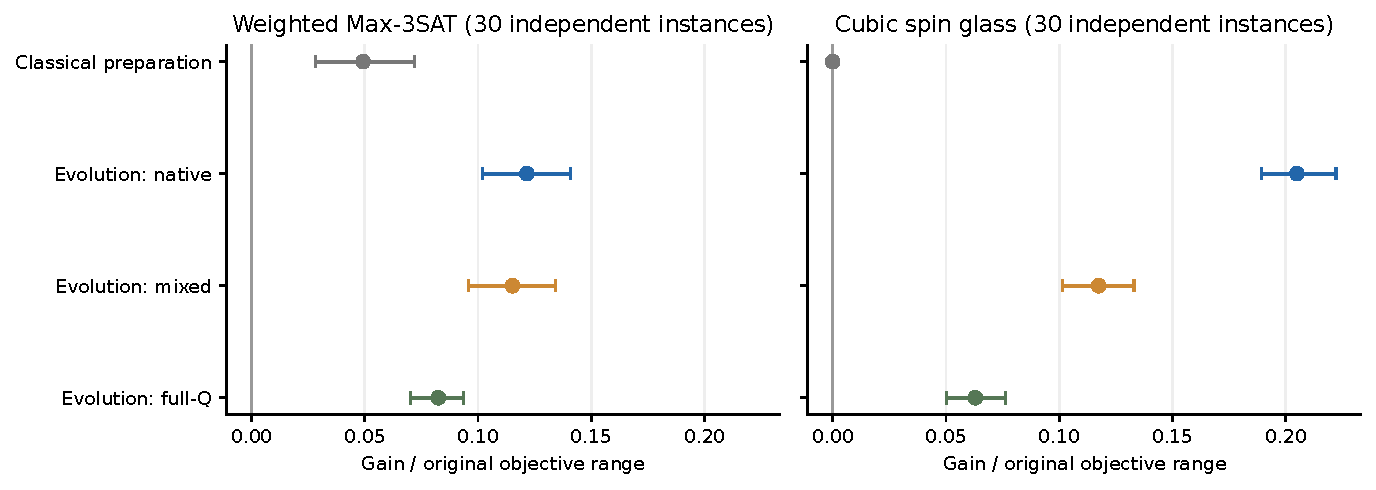
\includegraphics[width=\linewidth]{figures/revision_warm_gain_decomposition.pdf}

\caption{Classical preparation and subsequent $p=1$ evolution on fresh instances. Each gain is divided by its instance's exact original-objective range before averaging. Bars are paired instance-bootstrap 95\% intervals; positive values reduce the original objective. The incremental bars use the same warm $p=0$ comparator.}\label{fig:fresh-warm-decomposition}\end{figure}

For Weighted Max-3SAT, classical preparation changes the mean objective by 0.484 [0.279, 0.703], while native incremental evolution contributes 1.152 [0.959, 1.344]. The raw rounding, independent-sampling and prepared-state means are 2.267, 1.786 and 1.783, respectively.

Pair-moment warming relative to independence gives mean original-objective gains of 0.046 [-0.005, 0.112] for proper mixed and 0.119 [0.040, 0.202] for full-Q. These are secondary finite-budget contrasts, not a general pair-information advantage.

For Cubic spin glass, classical preparation changes the mean objective by 0.000 [0.000, 0.000], while native incremental evolution contributes 2.133 [2.004, 2.238]. The raw rounding, independent-sampling and prepared-state means are -1.467, 0.010 and 0.000, respectively.

Pair-moment warming relative to independence gives mean original-objective gains of -0.051 [-0.175, 0.061] for proper mixed and 0.112 [-0.011, 0.238] for full-Q. These are secondary finite-budget contrasts, not a general pair-information advantage.

\paragraph{Optimisation-budget sensitivity.} A separate $65\times65$ scan covers the full $(\gamma,\beta)$ domain, followed by four Nelder--Mead refinements with quotas of 240 evaluations each (5,185 objective evaluations in total per warm pair arm). Early termination in refinement uses the same prespecified uniform quota-completion rule. Integer encoded energies make the stated $2\pi$ phase period valid. A second equal-effort Nelder--Mead run uses the same three starts and $3\times120$ evaluations. The scan and refinements are an approximate-convergence sensitivity check, not a global-optimality certificate; the scan's zero-phase row includes the $p=0$ expectation.

\begin{table}[t]\centering\small\caption{Original-objective means for warm pair arms. EE: equal-effort COBYLA with quota completion; NM: equal-effort Nelder--Mead; scan: $65^2$ grid plus local refinement. Lower is better.}\label{tab:fresh-optimizer}

\begin{tabular}{llrrr}\toprule Family & Representation & EE & NM & Scan\\\midrule

Weighted Max-3SAT & Native & 0.631 & 0.772 & 0.405 \\

Weighted Max-3SAT & Proper mixed & 0.697 & 0.799 & 0.533 \\

Weighted Max-3SAT & Full-Q & 1.005 & 1.057 & 0.891 \\

Cubic spin glass & Native & -2.133 & -1.979 & -2.257 \\

Cubic spin glass & Proper mixed & -1.222 & -1.228 & -1.495 \\

Cubic spin glass & Full-Q & -0.648 & -0.535 & -0.888 \\

\bottomrule\end{tabular}\end{table}

The equal-effort COBYLA arms use 17,959 uniform-completion calls out of 172,800 objective evaluations. The second-optimiser and scan-refinement stages use 0 and 4,681 completion calls, respectively. All evaluation traces, early-stop messages and exact call counts are retained.

For Weighted Max-3SAT, the winning representation changes on 7/30 instances between equal-effort COBYLA and scanned refinement; the mean within-instance Spearman correlation across the three representations is 0.717. Switching to equal-effort Nelder--Mead changes the winner on 9/30. These changes limit conclusions drawn from one optimiser budget.

For Cubic spin glass, the winning representation changes on 1/30 instances between equal-effort COBYLA and scanned refinement; the mean within-instance Spearman correlation across the three representations is 0.917. Switching to equal-effort Nelder--Mead changes the winner on 2/30. These changes limit conclusions drawn from one optimiser budget.

\begin{figure}[t]\centering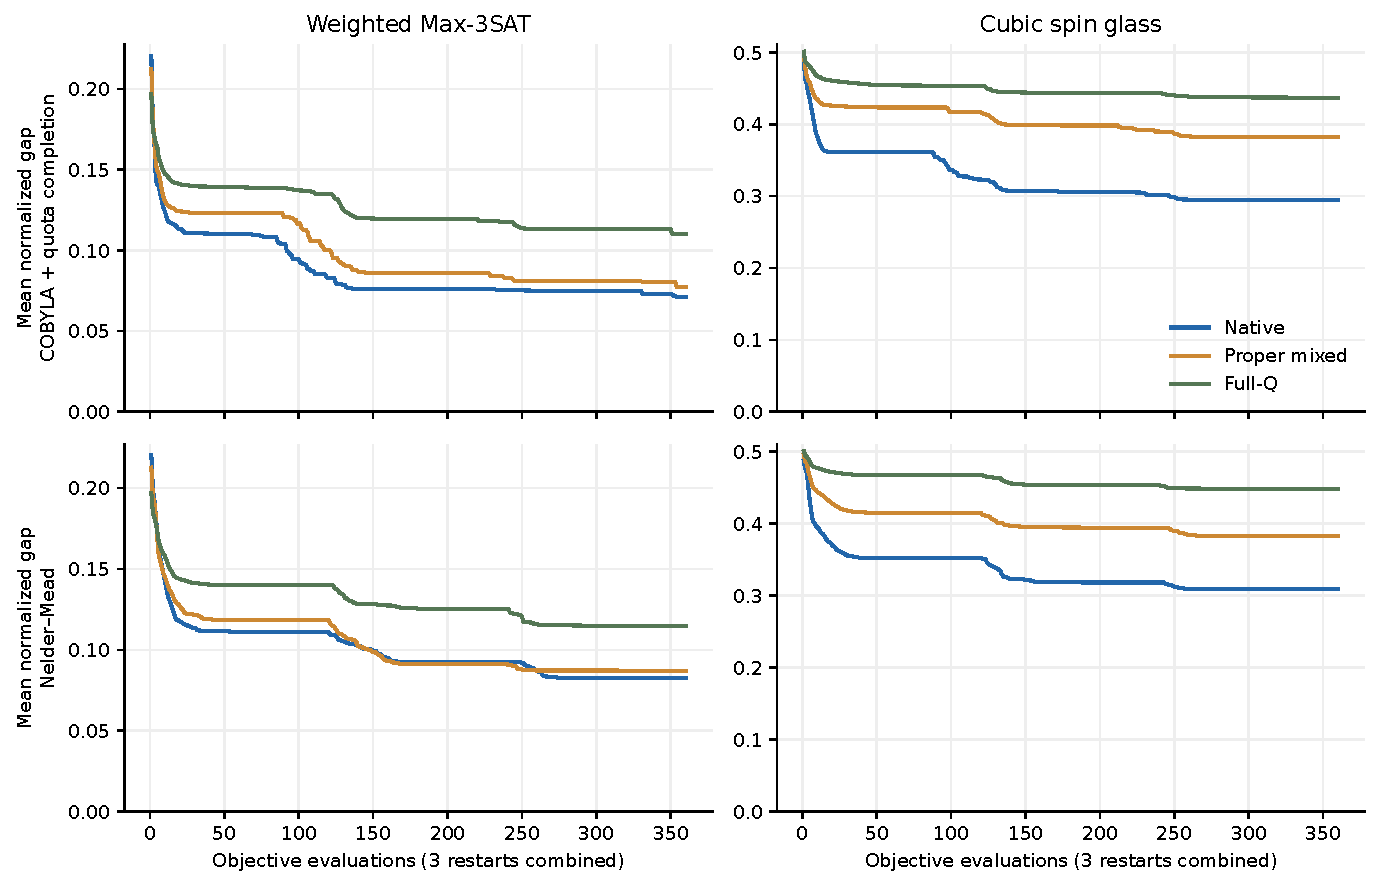
\includegraphics[width=.92\linewidth]{figures/revision_optimizer_curves.pdf}

\caption{Incumbent original-objective gap, divided by each instance's exact objective range, versus cumulative evaluations over three restarts. Each line averages 30 independent instances. All curves use pair warming. They distinguish equal-effort behaviour from the separately reported larger scan-and-refinement budget.}\label{fig:fresh-optimizer-curves}\end{figure}

The new evidence addresses independent-instance count and explicitly separates preparation from evolution, but only for small noiseless $p=1$ problems under the stated protocol. It establishes neither scalable quantum advantage nor a solution-quality advantage of mixed representations. Fibre guardrails remain optional appendix diagnostics whose predictive algorithmic utility is unresolved.
\subsection{Historical development studies}
We tested Max-3SAT and cubic spin-glass objectives on 60 oracle instances,
180 compilation instances and 14 noiseless QAOA instances, balanced between
the families. Comparisons use native, fully quadratized, selective and
matched-random representations; random controls match the number of active
auxiliaries. QAOA is scored on the original objective, ignoring auxiliary
bits. Resource differences are paired within instances; QAOA intervals use
instances, not restarts, as independent samples. Families are analysed
separately because their objective scales differ. The studies are exploratory;
generation, aggregation and execution details appear in
Methods (Section~\ref{sec:experiments}) and
Appendix~\ref{app:supplementary-results}.

\subsection{Development evidence: exactness and selector validation}
\label{sec:results-exactness}
\label{sec:results-selector-validation}

Exhaustive oracle checks found no pointwise mismatch above the analytical
penalty threshold, with unique, consistent minimising auxiliaries. At the
threshold, inconsistent assignments could tie without changing the minimum;
below it, explicit failures occurred. These results support the distinction
between exactness and strict consistency in
\cref{prop:cubic-mixed-sign}; Appendix~\ref{app:results-exactness}
reports complete counts.

The historical v2 Pareto beam satisfied its raw-moment guardrail on all 60
instances and matched the enumerated optimum in 58: all 30 spin-glass and
28 of 30 Max-3SAT cases. Maximum score regret was $0.010156$
(\cref{tab:selector-oracle-validation,fig:selector-oracle-summary}). The two
misses were training-labelled; all 12 test-labelled cases matched. The greedy
baseline matched the 30 spin-glass optima, which were native, but no Max-3SAT
optima. These are finite-space validation results for the historical diagnostic-constrained
feasible set. They do not certify the new resource-only selector or the new target compilers.

\begin{table}[!htbp]
\centering
\small
\caption{Oracle-tier validation on 60 instances. Regret is the selector
score minus the enumerated optimum. Certification is a separate exact run;
work and timing details are in Appendix~I.2.}
\label{tab:selector-oracle-validation}
\begin{tabular}{@{}lrrr@{}}
\toprule
Method & Zero-regret cases & Mean regret & Maximum regret\\
\midrule
Complete enumeration & 60/60 & 0 & 0\\
Pareto beam & 58/60 & $2.3003\times10^{-4}$ & 0.010156\\
Greedy native-completion & 30/60 & 0.019371 & 0.107292\\
Branch-and-bound certification & 60/60 & 0 & 0\\
\bottomrule
\end{tabular}

\end{table}

Separate branch-and-bound runs reached the enumerated optimum with zero
final gap on all 60 instances. Stored lower bounds were non-decreasing and
upper bounds non-increasing; 26 runs used certified capacity pruning, while
none used the conservative resource bound. This validates completed
small-instance certificates, without demonstrating better efficiency than
enumeration or large-instance scaling
(\cref{tab:selector-bnb-certification,fig:selector-bnb-gap}).
Certification is relative to the declared score, design grammar and fixed
all-to-all reference compiler. Device-level resources are assessed
afterwards, so these certificates do not establish optimality under every
hardware topology. Numerical certification uses the frozen floating-point moments
and the feasibility rule
$\widehat E_{\mathrm{fib}}^{\mathrm{computed}}\leq\tau_{\mathrm{fib}}+10^{-9}$.
It certifies this implemented set, rather than exact LP moments or zero-tolerance
feasibility.

Moderate beam-width and penalty-margin changes altered fewer selections
than resource weights or the fibre threshold. The guardrail removed all 12
recorded violations in the 48-case calibration ablation. Full sensitivity
results are in Appendix~I.2; QAOA was not rerun for
these sweeps.

\subsection{Development evidence: resource trade-offs}
\label{sec:results-resources}
\label{sec:results-regimes}

The selector repair changed 285 representation/draw groups across 65 fixed
compilation-tier instances. Under the unchanged compiler-seed and topology
protocols, 7,125 affected resource rows were rebuilt: 2,430 passed and 4,695
were expected width exclusions, with no unexpected compiler failure. The
remaining 23,475 observations retain their archived values and lineage.

All scheduled all-to-all compilations succeeded. Across 90 instances per
family, selective reduction lowers Max-3SAT median paired gate count by 25
and depth by 60.5 relative to native; for spin glass it lowers depth by 18
but adds six gates (\cref{tab:e2-all-to-all-paired}). Savings therefore
depend on the family and resource. This comparison pools split labels;
marginal levels and selector diagnostics are in
Appendix~\ref{app:results-resources}.

\begin{table}[!htbp]
    \centering
    \small
    \caption{Median within-instance resource difference from the native
    representation on the all-to-all topology.  Differences are calculated
    after transpiler-seed aggregation, so a negative value means a smaller
    circuit.  The table pools all 90 instances in each family.}
    \label{tab:e2-all-to-all-paired}
    \begin{tabular}{@{}llrr@{}}
        \toprule
        Family & Representation
        & $\Delta$ two-qubit gates & $\Delta$ two-qubit depth\\
        \midrule
        Max-3SAT & Fully reduced  & $-37$ & $-72$\\
                 & Selective      & $-25$ & $-60.5$\\
                 & Matched random & $+4$  & $-15.5$\\
        \addlinespace
        Cubic spin glass & Fully reduced  & $+42$ & $-29$\\
                         & Selective      & $+6$  & $-18$\\
                         & Matched random & $+8.2$ & $0$\\
        \bottomrule
    \end{tabular}
\end{table}

Width limits change which comparisons are possible. On the 12-qubit grid,
108 native designs fit, compared with 57 selective and 21 fully reduced
designs (\cref{tab:e2-sparse-capacity}). Only 21 instances fit all four
representations: 12 Max-3SAT and nine spin-glass cases. Direct grid
comparisons use this common subset, avoiding comparisons between different
success-only samples.

\begin{table}[!htbp]
    \centering
    \small
    \caption{Capacity results on the fixed 12-qubit sparse topology.  The
    counts refer to unique benchmark instances rather than compiler-seed
    rows.}
    \label{tab:e2-sparse-capacity}
    \begin{tabular}{@{}lrr@{}}
        \toprule
        Representation & Feasible instances & Fraction\\
        \midrule
        Native          & 108/180 & 60.0\%\\
        Fully reduced   & 21/180  & 11.7\%\\
        Selective       & 57/180  & 31.7\%\\
        Matched random  & 57/180  & 31.7\%\\
        \bottomrule
    \end{tabular}
\end{table}

\begin{table}[!htbp]
    \centering
    \small
    \caption{Median within-instance difference from native on the 21 instances
    that fit the sparse topology in all four representations.  Differences are
    calculated after seed aggregation; negative values mean lower resource
    use.}
    \label{tab:e2-sparse-common-paired}
    \begin{tabular}{@{}llrrrr@{}}
        \toprule
        Family & Representation
        & $\Delta$ gates & $\Delta$ depth & $\Delta$ SWAP & $\Delta$ routing\\
        \midrule
        Max-3SAT & Fully reduced  & $-16$ & $-29$ & $-3$   & $-5.5$\\
                 & Selective      & $-10$ & $-21$ & $-1.5$ & $-2$\\
                 & Matched random & $+6.5$ & $-3.9$ & $+1.8$ & $+4.8$\\
        \addlinespace
        Cubic spin glass & Fully reduced  & $+45$ & $+13$ & $+7$ & $+22$\\
                         & Selective      & $0$   & $0$   & $0$  & $0$\\
                         & Matched random & $0$   & $0$   & $0$  & $0$\\
        \bottomrule
    \end{tabular}

\end{table}

Within the common Max-3SAT subset, selective reduction saves a median of
10 gates and 21 depth units relative to native; matched random increases
gate count. This association is conditional on auxiliary count; reduced-term count,
penalty scale and the selection procedure remain possible confounders.
Eight of nine spin-glass selective designs are native, explaining the zero
selective and random medians, while full reduction increases every listed
resource. Only three common-fit instances are test-labelled, so these are
descriptive device-feasible results.
The random control deliberately matches auxiliary count rather than gate
count or penalty scale. It controls only register enlargement. Consequently, the historical advantage
does not isolate the causal value of partial reduction; the new controls match
both auxiliary count and the number of reduced cubic terms.

Line, ring and heavy-hex compilations reproduce the Max-3SAT
selective-versus-random pattern: depth decreases on every common-fit
instance, and gate count decreases on all line and ring cases and 54 of 55
heavy-hex cases. Spin-glass medians remain zero. The larger heavy-hex device
admits more instances, so these comparisons do not isolate connectivity
from capacity (Appendix~\ref{app:results-connectivity}).

\Cref{fig:e5-regime-map-2d} locates the savings against cubic sparsity and
pair reuse. The supplementary stability screen favours selective reduction
over matched random in 20 of 20 estimable Max-3SAT depth endpoints and
19 of 20 gate endpoints. These are descriptive endpoint counts, not
independent statistical samples. Sparse bins and capacity exclusions
prevent a universal inference that greater pair reuse guarantees larger
savings; complete counts appear in Appendix~\ref{app:results-regimes}.

\begin{figure}[!htbp]
    \centering
    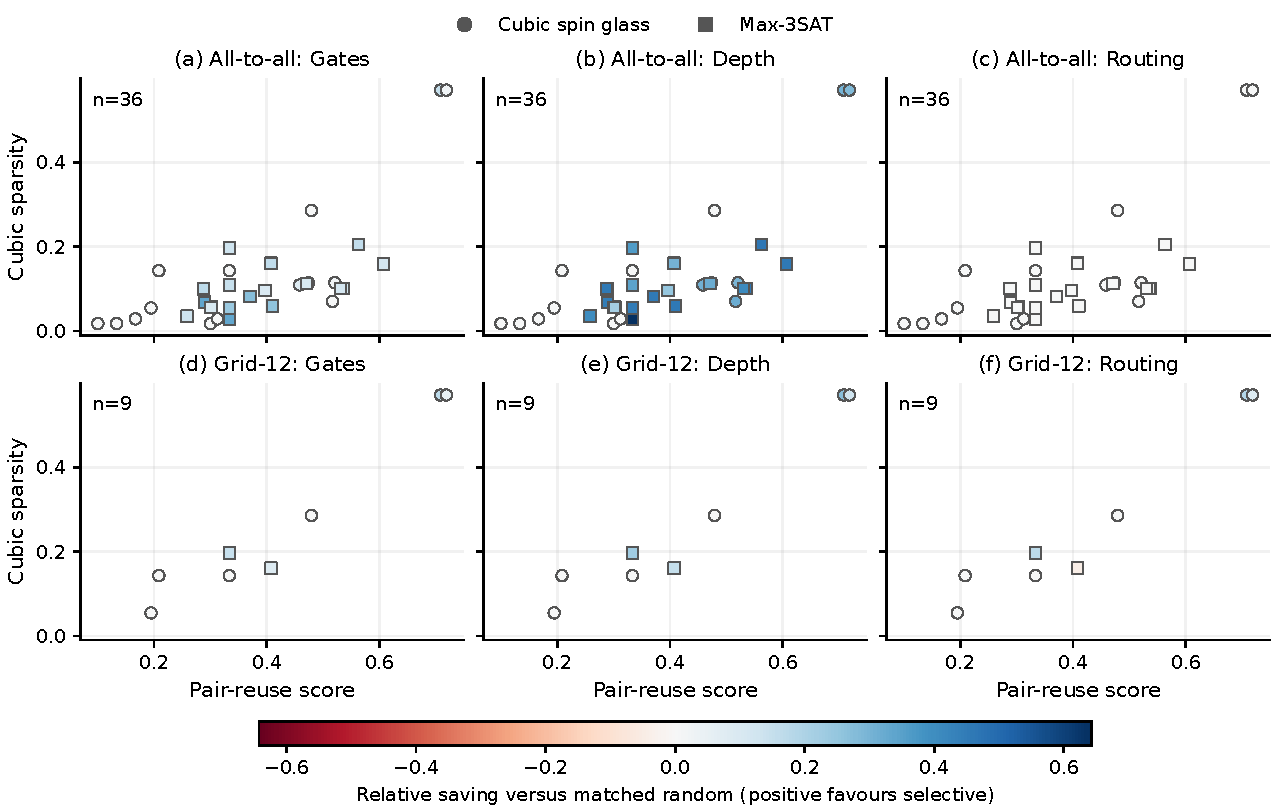
\includegraphics[width=\textwidth]{figures/figure_e5_regime_map_2d.pdf}
    \caption{Two-dimensional representation-regime map from the selector-repaired
    compilation results. Pair reuse and canonical cubic sparsity form the two axes. Panels (a)--(c) show
    all-to-all gates, depth, and routing; (d)--(f) show the same metrics on the
    fixed 12-qubit grid.  Colour is the relative saving of selective reduction over
    its matched-random control, so positive values favour the selective
    design.  Marker shape distinguishes the two benchmark families.}
    \label{fig:e5-regime-map-2d}
\end{figure}

\subsection{Boundary result: native quality under the historical budget}
\label{sec:results-qaoa}

On the 14 development instances (historically labelled test), native achieves the lowest mean
original-objective value at both depths $p=1,2$ and both gate budgets
$B=128,256$ in each family (\cref{tab:e3-qaoa-summary}). Circuit savings
therefore do not yield a general finite-depth QAOA advantage under this
optimisation protocol.

\begin{table}[!htbp]
    \centering
    \small
    \caption{Mean paired objective difference relative to the native
    representation in the noiseless QAOA study.  Lower is better, so positive
    entries favour the native representation.  Results from the two problem
    families are kept separate because their objective scales differ.}
    \label{tab:e3-qaoa-summary}
    \begin{tabular}{@{}llrrrr@{}}
        \toprule
        Family & Representation
        & $p=1$ & $p=2$
        & $B_{\mathrm{2q}}=128$
        & $B_{\mathrm{2q}}=256$\\
        \midrule
        Cubic spin glass
        & Fully reduced  & 1.837 & 2.041 & 2.044 & 2.458\\
        & Selective      & 0.379 & 0.275 & 0.431 & 0.821\\
        & Matched random & 0.394 & 0.271 & 0.448 & 0.543\\
        \addlinespace
        Max-3SAT
        & Fully reduced  & 1.774 & 2.112 & 0.245 & 1.855\\
        & Selective      & 1.899 & 1.935 & 0.040 & 1.511\\
        & Matched random & 1.390 & 1.192 & 0.385 & 1.516\\
        \bottomrule
    \end{tabular}
\end{table}

Four of eight selective-minus-native 95\% intervals include zero: spin-glass
at $p=1$, $p=2$ and $B=128$, and Max-3SAT at $B=128$. The Max-3SAT difference is
$1.935\;[0.597,3.273]$ at $p=2$, favouring native, and
$0.040\;[-1.013,1.093]$ at $B=128$; the spin-glass difference at $B=256$
is $0.821\;[0.007,1.635]$. An interval containing zero does not
establish equivalence.

The 128-gate comparison includes 35 of 112 design/draw groups, or 105
restart rows, with $p=0$: no complete cost layer fits the budget. These are
initial-state baselines, not optimised QAOA runs. Requiring every
representation and all random draws to fit at least one layer leaves five
spin-glass and three Max-3SAT instances. Their selective-minus-native
differences are $-0.072\;[-0.544,0.400]$ and
$0.982\;[-0.890,2.854]$, respectively. Both remain uncertain.
\Cref{tab:e3-b128-fit,fig:e3-secondary-metrics} provide the breakdown and
secondary diagnostics. Encoded energy and auxiliary inconsistency are
diagnostics; the optimised loss remains the original-objective expectation.

\subsection{Exploratory warm-start mechanisms and their limits}
\label{sec:results-warmstart}

Coordinate-corrected warm-start comparisons preserve the frozen instances,
LP probabilities and budgets. After selector repair, the execution audit
accounts for 4,176 original E4 rows and 480 targeted rows, including
validated zero-layer reuse and the removal of redundant warm policies for
newly zero-auxiliary designs;
Appendix~\ref{app:warmstart-correction-provenance} documents the correction
and provenance.
The corrected mixer uses the same angle convention as the cold baseline,
removing a coordinate mismatch from paired optimisation comparisons.
Original-variable warming and the incremental effect of warming auxiliaries
remain separate questions.

In the original E4 sample, 11 of 14 instances have weak median
original-variable bias,
$\operatorname{median}_i|\widehat\mu_i-1/2|\leq0.05$.
This statistic does not bound the full prepared state's distance from
uniformity. The common selective active-auxiliary comparison contains only
one spin-glass and seven Max-3SAT instances. Spin-glass intervals are not
estimable at $n=1$, while all four Max-3SAT primary pair-minus-cold intervals
include zero. Zero-layer cases remain labelled
at $B=128$ (\cref{tab:e4-warmstart-common,fig:e4-warmstart-corrected}).

\label{sec:results-strong-bias-warmstart}
The targeted study instead uses 20 strongest-screened instances, ten per
family, selected from relaxation information alone. Its 480 noiseless
runs at $p=1,2$ contain no zero-layer cases. This screened sample is
analysed separately and does not represent ordinary random instances.
Its LP optimum-selection provenance also differs from the original E4
sample; three selected spin-glass cases still fall below the single-variable
signal threshold (\cref{fig:e4-strong-bias-marginals}).

\begin{table}[!htbp]
\centering\small
\caption{Coordinate-corrected warm-start results on the 20 strongest-screened instances. Entries are mean paired original-objective differences with exploratory, unadjusted 95\% Student-$t$ intervals across ten raw instances per family, after averaging three restarts. Negative values favour the first policy named.}
\label{tab:e4-strong-bias-warmstart}
\resizebox{\textwidth}{!}{%
\begin{tabular}{@{}llrrr@{}}
\toprule
Family & Depth & Pair minus cold & Pair minus original-only & Pair minus independence\\
\midrule
Spin glass & $p=1$ & $-0.010\;[-0.281,0.260]$ & $-0.116\;[-0.344,0.112]$ & $-0.105\;[-0.320,0.109]$\\
Spin glass & $p=2$ & $0.152\;[-0.026,0.330]$ & $-0.025\;[-0.228,0.179]$ & $0.008\;[-0.289,0.304]$\\
Max-3SAT & $p=1$ & $-6.761\;[-9.263,-4.260]$ & $-0.149\;[-0.219,-0.080]$ & $0.092\;[-0.017,0.202]$\\
Max-3SAT & $p=2$ & $-6.722\;[-9.143,-4.300]$ & $-0.500\;[-0.875,-0.124]$ & $-0.153\;[-0.656,0.350]$\\
\bottomrule
\end{tabular}}
\end{table}

For targeted Max-3SAT, all three warm policies improve on cold start
(\cref{fig:e4-strong-bias-warmstart}). Pair-minus-cold differences are
$-6.761$ at $p=1$ and $-6.722$ at $p=2$, with intervals below zero.
Mean optimal-solution probability increases from $0.0360$ to $0.5987$
at $p=1$ and from $0.0419$ to $0.6262$ at $p=2$ under pair warming;
these probabilities are secondary diagnostics. Spin-glass differences
remain uncertain.

The Max-3SAT pair-minus-original-only differences are
$-0.149\;[-0.219,-0.080]$ at $p=1$ and
$-0.500\;[-0.875,-0.124]$ at $p=2$.
Both pair-minus-independence intervals include zero. The unadjusted
intervals therefore support an exploratory benefit over
original-only warming at both depths, without establishing a stable
additional benefit over independence-based auxiliary warming.
The limited noise study is reported separately in
Appendix~\ref{sec:results-noise}.

\FloatBarrier

\section{Discussion}
\label{sec:discussion}
\label{sec:conclusion}
\label{sec:discussion-search-scope}

Exact selective locality reduction makes representation choice explicit
without changing the represented classical objective. The sharp
aggregate-residual penalty and composition theorem establish this property
independently of the numerical experiments. The cubic construction then
exposes a resource trade-off within one exact family: sharing an auxiliary
can lower locality across several terms, but also introduces qubit, coupling
and penalty costs. The value of selectivity is the ability to balance these
costs under a stated compilation protocol. Exactness alone does not predict
which representation will have the smallest circuit or the best variational
performance. At fixed depth, QAOA can depend on local graph
structure~\cite{WangMaxCut2018,FarhiLocal2020} and constraint
density~\cite{Akshay2020}. These results motivate studying the circuit
changes caused by reformulation, but do not predict our representation
rankings.

The new compilation study strengthens an existence claim: measured mixed circuits can satisfy joint budgets while exhaustive logical enumeration excludes the entire full endpoint and native violates compiled cost limits. It also narrows its practical scope. An unrestricted weighted score chose native in every random-instance setting, and a stronger gadget ordering removed the observed spin-glass mixed-only regions. High rank correlations coexisted with changing Pareto sets and full assignments. Thus hard budgets, target-specific selection and the declared synthesis are substantive parts of the result, not incidental implementation details.

The new QAOA study separates two different sources of improvement. Native incremental evolution is positive on all 30 instances of each family under the frozen equal-effort protocol, while preparation itself gives measurable average benefit only for Max-3SAT. Yet native also has the best mean original objective under the second optimiser and the larger scan/refinement budget. Some individual winners change as optimisation effort increases. These small, noiseless findings support a boundary between executable representation and variational quality; they neither establish a mixed quality advantage nor a scalable quantum advantage.

The historical resource results support this distinction. Max-3SAT showed the clearest
benefits, whereas the spin-glass data exhibited a gate--depth trade-off.
Reuse of variable pairs offers a plausible explanation for this structural
dependence, but the regime maps are descriptive rather than predictive.
The repeated Max-3SAT advantage over matched-random reduction on additional
coupling maps extends the evidence beyond the original grid. However,
different capacities and embeddings change which instances fit in every
representation. Common-fit comparisons therefore assess circuit resources
within each eligible subset; they do not isolate connectivity from capacity
or establish a topology-independent ranking.

Smaller circuits did not yield a general improvement in noiseless QAOA.
The native representation had the best mean original-objective value in both
families over the full scheduled comparison. That comparison includes
zero-layer states when the gate budget cannot accommodate a layer; these
remain useful capacity outcomes but cannot be interpreted as completed
positive-depth optimisations. Restricting to instances where all
representations admit a layer leaves a small, inconclusive comparison.
The supplementary noise experiment likewise distinguishes starting quality
from degradation: a representation changing less from an already worse
noiseless value is not necessarily preferable. Its representative simulator
parameters do not establish robustness on a calibrated device.

Warm-start behaviour also depends on the state and mixer: failure of
standard QAOA initialised at a good classical string~\cite{Cain2023}
does not establish failure of the matched product-state schemes used here.
The warm-start findings depend on both the available relaxation signal and
the comparison population. The original sample gives no clear primary
pair-versus-cold advantage after coordinate correction. Weak median
original-variable bias helps characterise that sample, but does not bound
every marginal or the distance of the full prepared register from a uniform
state. On the deliberately signal-enriched Max-3SAT subset, all three warm
policies improve over cold start. Pair warming additionally improves over
original-only warming at both depths in unadjusted exploratory contrasts.
The pair-versus-independence contrasts remain inconclusive, so the study does
not isolate a general benefit from direct auxiliary pair moments. The
spin-glass warm-start evidence also remains uncertain.

The coordinate correction aligns the warm and cold mixer conventions for
paired optimisation. It was executed in a different numerical environment,
requiring the positive-depth cold controls to be rerun as well. Changes
between historical and corrected outcomes consequently cannot be attributed
solely to the mixer convention. The original and targeted studies also
retain different archived choices of the LP optimum representative and
must be interpreted separately. In particular, the targeted selective-only
sample cannot be pooled with the original four-representation benchmark
to estimate performance on ordinary random instances.

The historical numerical scope is limited: that QAOA comparison uses
14 instances, the targeted warm-start study uses 20, and the noise study
uses 18. Small active-auxiliary subsets further limit paired comparisons.
The historical 60-instance oracle study validates completed searches under the fixed
reference synthesis and recorded numerical feasibility rule, without
establishing search scaling. A certificate concerns that declared design
space and objective; an uncertified incumbent is only the best design
found. The relaxation-derived fibre diagnostic is now optional and excluded from
primary selection. Compliance with its threshold does not establish
predictive or algorithmic utility.
Additional compilation targets extend the resource analysis only, rather
than the QAOA or noise evidence.

The new phase theorem identifies a stronger utility than occupying an intermediate point: within its declared grammar and budgets, every feasible representation can be mixed. This does not exclude nonsemantic auxiliaries or other quadratization grammars. The compiled corollary depends on its fixed synthesis, and the compiler study tests rather than assumes robustness to ordering and connectivity. Joint-budget feasibility without a solution-quality constraint means executable exact representation, not a demonstrated useful approximation ratio or quantum advantage. No quality-threshold feasibility claim is made without sufficient new quality data.

The framework therefore supplies a controlled way to compare exact
representations rather than a universally preferred encoding. Beyond
cubic objectives, the exactness theory already applies, but substitution
order changes reuse, penalties and compilation cost, requiring a larger
design search. Future evaluation should test how these choices interact
with relaxation information and finite-depth performance on larger,
independently selected instances. Such work would distinguish reproducible
resource savings from the stronger claim of improved optimisation quality.

\section{Methods}
\label{sec:methodology}
\label{sec:experiments}

\subsection{Resource-aware selection and certification}
\label{sec:selection}
\label{sec:selection-problem}
\label{sec:search-certification}

Fix the compilation protocol $\Pi$, including architecture, synthesis,
compiler seeds and aggregation. For positive scales and nonnegative weights
summing to one, rank designs by
\begin{equation}
J_{\mathrm{res}}(\sigma)=
w_a\frac{a_\sigma}{s_a}+w_G\frac{G_{2q,\sigma}}{s_G}
+w_D\frac{D_{2q,\sigma}}{s_D}+w_M\frac{M_{\max,\sigma}}{s_M}.
\label{eq:Jres}
\end{equation}
Gate count and depth come from the declared compiler, rather than polynomial
degree alone~\cite{Verchere2023,Weidenfeller2022,Schmidbauer2024}.
The primary selector uses resource constraints only. Selection must call the compiler for the target topology being evaluated; historical all-to-all certificates are kept as validation of that historical model. New searches are finite-budget heuristics unless an exhaustive certificate is explicitly stated.

The fibre quantity $E_{\mathrm{fib}}=\mathbb E[F_\sigma(X,Y)-f(X)]$ is retained solely as an optional heuristic diagnostic in Appendix~\ref{app:fibre-risk}. Raw pseudo-moments and the clipped probabilities actually used for preparation define different product laws. Neither diagnostic has established predictive value for final quality or consistency after controlling for width, gates and depth. Its algorithmic utility remains unresolved, and it is excluded from primary selection.
\begin{equation}
E_{\mathrm{fib}}(\sigma;\eta,\xi)=\mathbb E[F_\sigma(X,Y)-f(X)]\geq0,
\qquad \widehat E_{\mathrm{fib}}=E_{\mathrm{fib}}/s_{\mathrm{fib}}.
\label{eq:fibre-excess-short}
\end{equation}
Here the original and auxiliary bits are independently Bernoulli with parameters $(\eta,\xi)$ and $s_{\mathrm{fib}}>0$ is design independent. This definition does not assert a joint distribution for raw pseudo-moments.

The feasible set and optimisation target are
\begin{equation}
\mathcal F_{\mathrm{sel}}=\left\{\sigma\in\Sigma_{\mathrm{ex}}^\varepsilon:
\begin{array}{c}
N_\sigma\leq Q_{\max},\ G_{2q,\sigma}\leq B_G,\ D_{2q,\sigma}\leq B_D,\\
M_{\max,\sigma}\leq B_M
\end{array}\right\},
\label{eq:selection-feasible-set}
\end{equation}
\begin{equation}
J_{\mathrm{res}}^\star=\min_{\sigma\in\mathcal F_{\mathrm{sel}}}J_{\mathrm{res}}(\sigma).
\label{eq:selection-problem}
\end{equation}
The minimum is attained whenever $\mathcal F_{\mathrm{sel}}$ is nonempty.
To isolate the freedom to retain terms, compare
\begin{equation}
\min_{\rho:(E,\rho)\in\mathcal F_{\mathrm{sel}}}J_{\mathrm{res}}(E,\rho)
\quad\hbox{with}\quad
\min_{\mathcal D,\rho:(\mathcal D,\rho)\in\mathcal F_{\mathrm{sel}}}J_{\mathrm{res}}(\mathcal D,\rho).
\label{eq:fair-full-comparison}
\end{equation}
The full family is a subset of the selective family, so exact optimisation cannot worsen the latter's best score. Under finite search budgets that ordering is not guaranteed: report incumbent costs and actual compiler calls, not an unearned optimum. Minimum-auxiliary full reduction instead isolates the effect of changing the resource objective. Maximum reuse tests a simple structural rule; a hardware-aware rule tests the value of explicit device information. Random controls matched on both $a_\sigma$ and $|\mathcal D|$ test choices within that structural stratum. They still do not hold penalty or pair-reuse distribution fixed.

% Required in the preamble (TikZ is already loaded by quantikz):
% \usetikzlibrary{arrows.meta,shapes.geometric}
% Vector artwork; no external image or shell escape is required.
\begin{figure}[tbp]
\centering
\begin{tikzpicture}[
  x=\textwidth,y=1cm,
  font=\footnotesize,
  box/.style={draw=black!65,rounded corners=2pt,fill=black!2,
    align=center,text width=.265\textwidth,inner sep=5pt,
    minimum height=1.02cm},
  result/.style={box,fill=blue!4,draw=blue!55!black},
  decision/.style={diamond,aspect=2.3,draw=black!65,
    fill=black!2,align=center,inner sep=3pt},
  arr/.style={-{Stealth[length=2mm,width=1.4mm]},thick,draw=black!75}
]
\node[box] (input) at (.165,0)
  {\textbf{Fix the problem}\\
   Exact family and protocol\\Score and budgets};
\node[box] (seed) at (.5,0)
  {\textbf{Evaluate references}\\
   Native and fully reduced\\Update feasible incumbent};
\node[box] (beam) at (.835,0)
  {\textbf{Pareto-beam search}\\
   Score completions\\Keep up to $B$ prefixes};
\node[decision] (certify) at (.835,-1.65)
  {Certify?};
\node[box] (bnb) at (.5,-1.65)
  {\textbf{Branch and bound}\\
   Root frontier; reuse records\\Admissible pruning only};
\node[result] (certified) at (.5,-3.25)
  {\textbf{Return design / status}\\
   Certified bounds\\Gap, if bounds are finite};
\node[result] (heuristic) at (.835,-3.25)
  {\textbf{Return heuristic result}\\
   Incumbent, if found\\No optimality certificate};
\draw[arr] (input) -- (seed);
\draw[arr] (seed) -- (beam);
\draw[arr] (beam) -- (certify);
\draw[arr] (certify) -- node[above,font=\scriptsize]{yes} (bnb);
\draw[arr] (certify) -- node[right,font=\scriptsize]{no} (heuristic);
\draw[arr] (bnb) -- (certified);
\end{tikzpicture}
\caption{Representation selection separates a practical search from optional
certification. The beam seeks a low-cost feasible design; its discarded
prefixes remain part of the certification search. Branch and bound may
return an optimal, infeasible or interrupted status, with bounds reported
according to the stopping rules in Appendix~\ref{app:selection-implementation}. The historical optional fibre constraint is not part of the primary selector.}
\label{fig:selector-workflow}
\end{figure}

Each cubic term has four actions: remain native or use one of its three
pairs. A width-$B$ Pareto beam explores this finite action tree and updates
the best feasible design, or \emph{incumbent}. Its truncations can miss better
designs. Optional branch and bound~\cite{LandDoig1960,LawlerWood1966}
therefore restarts from the root, reuses
evaluations, and excludes a subtree only through proved infeasibility or a
valid lower bound. In particular, an infeasible native completion does not
make every descendant infeasible.

Let $U_J$ be the incumbent score and $L_J^{\mathrm{glob}}$ the minimum of
$U_J$ and the admissible bounds on the unresolved frontier. With frontier
coverage preserved and a finite incumbent,
\begin{equation}
L_J^{\mathrm{glob}}\leq J_{\mathrm{res}}^\star\leq U_J,
\qquad U_J-J_{\mathrm{res}}^\star\leq U_J-L_J^{\mathrm{glob}}.
\label{eq:anytime-certificate}
\end{equation}
Equality certifies the optimal value only for the declared design space,
compiler and constraints. Without an incumbent, the search reports that
none has yet been found; infeasibility requires exhausting the frontier.
Figure~\ref{fig:selector-workflow} summarises the procedure.
The historical Algorithm~\ref{alg:selector} includes an optional fibre check;
it is disabled for the primary resource-only problem. Its admissible bounds, numerical requirements and
the proof of Proposition~\ref{prop:anytime-certificate} are in
Appendix~\ref{app:certified-selection}.

\subsection{Warm-started QAOA and evaluation}
\label{sec:warm-start}
\label{sec:warm-start-state}
\label{sec:ws-qaoa}
\label{sec:cost-consistency}

For the selected representation, construct a product warm start from the
same relaxation~\cite{Egger2021,TateSDP2023,TateCustom2023}.
Set $\mu_i=\operatorname{clip}_\delta(\bar\mu_i)$, where
$\operatorname{clip}_\delta(t)=\min\{1-\delta,\max\{\delta,t\}\}$ and
$0<\delta<1/2$. Use $q_p=\operatorname{clip}_\delta(\bar q_{ij})$ when
pair moments are available; the independence fallback $q_p=\mu_i\mu_j$
is not clipped again. With
$|\phi(t)\rangle=\sqrt{1-t}|0\rangle+\sqrt t|1\rangle$,
\begin{equation}
|\Phi_\sigma^{\mathrm{ws}}\rangle=
\bigotimes_{i=1}^n|\phi(\mu_i)\rangle
\otimes\bigotimes_{p\in P_\rho}|\phi(q_p)\rangle.
\label{eq:ws-state}
\end{equation}
For its ordered probabilities $\omega=(\mu,q)$, define
\begin{equation}
H_{M,\sigma}^{\mathrm{ws}}=\sum_{j=1}^{N_\sigma}h_M^{(j)}(\omega_j),
\qquad h_M(t)=-2\sqrt{t(1-t)}X-(1-2t)Z.
\label{eq:ws-mixer}
\end{equation}
The warm state is its unique ground state. We use
$U_F(\gamma)=e^{-i\gamma H_{F_\sigma}}$ and
$U_M(\beta)=e^{+i\beta H_{M,\sigma}^{\mathrm{ws}}}$, so uniform probabilities
on \emph{every} qubit recover the cold mixer
$e^{-i\beta\sum_jX_j}$ at the same optimiser coordinates. The depth-$r$ ansatz is
\begin{equation}
|\psi_{r,\sigma}\rangle=
U_M(\beta_r)U_F(\gamma_r)\cdots U_M(\beta_1)U_F(\gamma_1)
|\Phi_\sigma^{\mathrm{ws}}\rangle,
\label{eq:method-qaoa-ansatz}
\end{equation}
with $r=0$ denoting the initial state. All cost terms commute, so cost-layer
factorisation is exact. The local mixer can leave the consistent subspace;
penalties do not guarantee consistent measurement outcomes.
Feasible-subspace mixers offer a different design choice within the
quantum alternating operator framework~\cite{Hadfield2019}.

Optimisation and solution quality use the original-objective expectation,
$\mathcal E_f(\psi)=\sum_{x,y}f(x)\,p_\psi(x,y)$, where
$p_\psi(x,y)=|\langle x,y|\psi\rangle|^2$.
Optimal-solution probability also sums over all auxiliary outcomes.
Auxiliary inconsistency is a separate diagnostic,
$R_{\mathrm{inc}}=\mathbb P_\psi(Y\neq\phi_\rho(X))$, set to zero when no
auxiliaries are present. Circuit identities, consistency definitions and
the raw-versus-clipped diagnostic check are in
Appendix~\ref{app:warm-start-circuits}; budgets and aggregation are specified
below and in the technical appendices.

% New subsection labels avoid collisions with the retained technical details.
% Suggested migration: retain the original application/formulation labels in
% the technical appendices; use these new equations for the concise main text.
\subsection{Benchmark construction and comparison protocol}
\label{sec:benchmark-protocol}

Weighted Max-3SAT minimises the total violated-clause weight,
\begin{equation}
 f_{\mathrm{3SAT}}(\bm x)=\sum_C w_C\prod_{\ell_i\in C}u_{\ell_i}(x_i),
 \qquad w_C>0,
 \label{eq:methods-max3sat}
\end{equation}
where $u_{x_i}=1-x_i$ and $u_{\neg x_i}=x_i$. The complementary spin-glass
benchmark uses
\begin{equation}
 E(\bm s)=\sum_{\{i,j,k\}\in\mathcal E}K_{ijk}s_is_js_k,
 \qquad s_i\in\{-1,1\},\quad K_{ijk}\in\{-1,1\},
 \label{eq:methods-cubic-spin}
\end{equation}
with a sampled set of triples $\mathcal E$. We use $s_i=1-2x_i$ and
aggregate equal monomials
before reduction. Sampling varies sparsity and pair reuse; the families are
contrasting benchmarks, not a controlled separation of application and
hypergraph effects. Generation and expansion details appear in
Appendices~\ref{app:benchmark-generation}, \ref{app:max3sat}
and~\ref{app:spin-glass}.

The historical development tiers contain 60 oracle instances, 180 compilation instances
and 14 test-labelled noiseless-QAOA instances, balanced between families.
Oracle checks exhaustively compare $f(\bm x)$ with
$\min_{\bm y}F_\sigma(\bm x,\bm y)$ and test threshold tightness and consistency.
Separate studies use 18 noise instances and 20 strongest-screened warm-start
instances. The latter are selected using relaxation information alone, without
QAOA outcomes; they are not a representative random sample and are not pooled
with the original comparison. Evaluated samples differ from candidate-pool
generation targets.

In those historical tiers, each raw instance has native, fully quadratized, selective and matched-random
representations. Full reduction uses a minimum-cardinality pair cover with
deterministic tie-breaking. Five seeded random controls match only the number
of active auxiliaries; they need not be distinct or match compiled resources.
Construction and fallback rules are in Appendix~\ref{app:experimental-controls}.
The recorded within-family, within-tier split is $60\%/20\%/20\%$ for
training, validation and test. Settings were chosen using training and
validation data, without direct selector retuning on test-labelled rows.
However, the pool was available during protocol refinement, so this remains
exploratory rather than an untouched-test evaluation. Resource comparisons
pool all 180 compilation instances.

The historical representations use common synthesis settings and five transpiler seeds
on all-to-all coupling and a 12-qubit $3\times4$ grid. We record register
width, two-qubit gates and depth, routing, penalties and coefficient range.
Width failures are recorded separately; paired device comparisons use the
common-fit subset. Additional line, ring and heavy-hex comparisons evaluate
selective and random designs without rerunning QAOA
(Appendices~\ref{app:hardware-compiler-protocol} and~\ref{app:reproducibility}).

Historical QAOA runs used COBYLA~\cite{Powell1994},
three restarts,
at most 60 objective evaluations per restart and tolerance $10^{-3}$.
The loss is the original-objective expectation $\mathcal E_f$, ignoring
auxiliary outcomes; encoded energy and consistency are diagnostics.
Angles are initialised with $\gamma\in[0,2\pi]$ and $\beta\in[0,\pi]$;
these are initialisation intervals, not optimisation bounds. Equal-layer
comparisons use $p=1,2$. For gate budgets $B\in\{128,256\}$ and median
grid cost-layer count $g_\sigma>0$, the assigned depth is
\begin{equation}
 p_\sigma(B)=\left\lfloor B/g_\sigma\right\rfloor.
 \label{eq:methods-gate-budget}
\end{equation}
Zero-layer cases remain as initial-state baselines with no trainable
parameters; their counts and the subset fitting a layer in every design are
reported separately. The targeted warm-start study contains only $p=1,2$.

Primary QAOA results use exact statevector expectations. E6 uses 4096 shots
per evaluation and representative depolarising and readout errors on the grid,
not a calibrated device. Its initial depth from
\cref{eq:methods-gate-budget} is decreased until the complete transpiled,
measured circuit fits the budget. Realised depths are used in comparisons.
Noiselessly optimised parameters are reused at both noise levels without
re-optimisation (Appendix~\ref{app:noise-protocol}).

\subsection{Statistics and reproducibility}
\label{sec:statistics-reproducibility}

The raw instance is the statistical unit. In the historical studies, resource aggregation first takes
the median over transpiler seeds for each design, then averages the five
random-control design values within each instance. QAOA aggregation averages
three restarts per design, then the random-design means. Paired differences
are formed afterwards; no best-seed, best-restart or best-draw selection is
used. Resource summaries report medians of paired instance differences.
QAOA, warm-start and noise summaries report means and two-sided 95\%
Student-$t$ intervals~\cite{Student1908} across instances.

Corrected warm-start intervals use $n-1$ degrees of freedom and are
unadjusted for multiple comparisons. These exploratory intervals, especially
for small samples, do not establish equivalence when they include zero.
Repeated seeds and restarts are not independent samples. Descriptive regime
labels use a separate within-endpoint stability rule
(Appendix~\ref{app:experimental-statistics}).

The warm-start coordinate correction preserves frozen instances, designs,
archived probability vectors, initial parameters, seeds, budgets and loss.
It neither resolves the LP nor screens new instances. Positive-depth cold
comparisons were rerun because optimiser-environment equivalence was not
established; zero-layer reuse was validated. Historical and corrected results
are not pooled. Original E4 uses the first HiGHS optimum, whereas selection
and targeted screening use a deterministic optimum-face representative.
Full solver rules, execution provenance and reconstruction records are
retained in Appendices~\ref{app:experimental-lp},
\ref{app:optimisation-hyperparameters}
and~\ref{app:warmstart-correction-provenance}.

\FloatBarrier
\section*{Data availability}
The new evaluation data, frozen protocols, execution records and analysis scripts
are supplied in the accompanying revision code-and-evidence archive. They have
not been represented as uploaded to the public repository. The historical
processed data and source manifests
are available in the
\href{https://github.com/rrocy6/urss-selective-locality-reduction}{project
repository}. The complete raw data for the warm-start coordinate correction are publicly
archived in the
\href{https://github.com/rrocy6/urss-selective-locality-reduction/blob/efaa1ce60fbc9984006472c4b2672578027fac78/delivery/20260913/archives/URSS_WARMSTART_CORRECTION_EXECUTED_v1.zip}{versioned correction archive}.
The archive identity and SHA-256 are recorded in
Appendix~\ref{app:reproducibility}. 

\section*{Code availability}
The new resource and QAOA evaluation code and its reproduction instructions
are included with this revision. Historical code, together with the
environment information and reproduction instructions, is available in the
\href{https://github.com/rrocy6/urss-selective-locality-reduction}{project
repository}.

\section*{Acknowledgments}
The authors thank H. M. Waseem, Carsten Maple and Bo Chen for valuable discussions and guidance. This work was supported by the University of Warwick Undergraduate Research Support Scheme (URSS).

\section*{Author contributions}
J.L. conceived the study, developed the theoretical framework, derived the analytical results and wrote the manuscript. Y.S. and R.Z. designed and implemented the numerical experiments, analysed the data and contributed to the interpretation of the results. All authors contributed to the manuscript; this revision remains subject to their review and approval.

\section*{Competing interests}
The authors declare no competing interests.

\begingroup
\small
\begin{thebibliography}{99}

\bibitem{BorosHammer2002}
Endre Boros and Peter~L. Hammer.
\newblock ``Pseudo-boolean optimization''.
\newblock \href{https://dx.doi.org/10.1016/S0166-218X(01)00341-9}{Discrete Applied Mathematics {\bf 123}, 155--225}~(2002).

\bibitem{Hadfield2021}
Stuart Hadfield.
\newblock ``On the representation of Boolean and real functions as Hamiltonians for quantum computing''.
\newblock \href{https://dx.doi.org/10.1145/3478519}{ACM Transactions on Quantum Computing {\bf 2}, Article 18, 1--21}~(2021).
\newblock \href{http://arxiv.org/abs/1804.09130}{arXiv:1804.09130}.

\bibitem{Farhi2014}
Edward Farhi, Jeffrey Goldstone, and Sam Gutmann.
\newblock ``A quantum approximate optimization algorithm''~(2014).
\newblock \href{http://arxiv.org/abs/1411.4028}{arXiv:1411.4028}.

\bibitem{Zhou2020}
Leo Zhou, Sheng-Tao Wang, Soonwon Choi, Hannes Pichler, and Mikhail D. Lukin.
\newblock ``Quantum Approximate Optimization Algorithm: Performance, Mechanism, and Implementation on Near-Term Devices''.
\newblock \href{https://doi.org/10.1103/physrevx.10.021067}{Physical Review X {\bf 10}, 021067}~(2020).


\bibitem{Glos2022}
Adam Glos, Aleksandra Krawiec, and Zolt{\'a}n Zimbor{\'a}s.
\newblock ``Space-efficient binary optimization for variational quantum computing''.
\newblock \href{https://dx.doi.org/10.1038/s41534-022-00546-y}{npj Quantum Information {\bf 8}, 39}~(2022).
\newblock \href{http://arxiv.org/abs/2009.07309}{arXiv:2009.07309}.

\bibitem{CampbellDahl2022}
Colin Campbell and Edward Dahl.
\newblock ``QAOA of the highest order''.
\newblock In 2022 IEEE 19th International Conference on Software Architecture Companion (ICSA-C), pages 141--146~(2022).
\newblock \href{https://dx.doi.org/10.1109/ICSA-C54293.2022.00035}{doi:10.1109/ICSA-C54293.2022.00035}.
\newblock \href{http://arxiv.org/abs/2111.12754}{arXiv:2111.12754}.

\bibitem{Stein2023}
Jonas Stein, Farbod Chamanian, Maximilian Zorn, Jonas N{\"u}{\ss}lein, Sebastian Zielinski, Michael K{\"o}lle, and Claudia Linnhoff-Popien.
\newblock ``Evidence that PUBO outperforms QUBO when solving continuous optimization problems with the QAOA''.
\newblock In Proceedings of the Genetic and Evolutionary Computation Conference Companion.
\newblock \href{https://dx.doi.org/10.1145/3583133.3596358}{Pages 2254--2262}~(2023).
\newblock \href{http://arxiv.org/abs/2305.03390}{arXiv:2305.03390}.

\bibitem{Bell2025}
Kristina Bell, Adam Lowe, Emily Coles, Nathanael Ridgway, and Gillian Marshall.
\newblock ``A comparison of quadratic and higher-order representations for QAOA''~(2025).
\newblock \href{http://arxiv.org/abs/2509.20127}{arXiv:2509.20127}.

\bibitem{Dragoi2026}
Sabina Dr{\u a}goi, Alberto Baiardi, and Daniel~J. Egger.
\newblock ``Approximate quadratization of high-order Hamiltonians for combinatorial quantum optimization''.
\newblock Physical Review Research {\bf 8}, 023159~(2026).
\newblock \href{http://arxiv.org/abs/2505.04700}{arXiv:2505.04700}.

\bibitem{Verchere2023}
Zo{\'e} Verch{\`e}re, Sourour Elloumi, and Andrea Simonetto.
\newblock ``Optimizing variational circuits for higher-order binary optimization''.
\newblock In 2023 IEEE International Conference on Quantum Computing and Engineering (QCE), volume 1, pages 19--25~(2023).
\newblock \href{https://dx.doi.org/10.1109/QCE57702.2023.00011}{doi:10.1109/QCE57702.2023.00011}.
\newblock \href{http://arxiv.org/abs/2307.16756}{arXiv:2307.16756}.

\bibitem{Weidenfeller2022}
Johannes Weidenfeller, Lucia~C. Valor, Julien Gacon, Caroline Tornow, Luciano Bello, Stefan Woerner, and Daniel~J. Egger.
\newblock ``Scaling of the quantum approximate optimization algorithm on superconducting qubit based hardware''.
\newblock \href{https://dx.doi.org/10.22331/q-2022-12-07-870}{Quantum {\bf 6}, 870}~(2022).
\newblock \href{http://arxiv.org/abs/2202.03459}{arXiv:2202.03459}.

\bibitem{Harrigan2021}
Matthew P. Harrigan et al.
\newblock ``Quantum approximate optimization of non-planar graph problems on a planar superconducting processor''.
\newblock \href{https://doi.org/10.1038/s41567-020-01105-y}{Nature Physics {\bf 17}, 332--336}~(2021).


\bibitem{Rosenberg1975}
I.~G. Rosenberg.
\newblock ``Reduction of bivalent maximization to the quadratic case''.
\newblock Cahiers du Centre d'\'Etudes de Recherche Op\'erationnelle {\bf 17}, 71--74~(1975).

\bibitem{BorosGruber2014}
Endre Boros and Aritanan Gruber.
\newblock ``On quadratization of pseudo-boolean functions''~(2014).
\newblock \href{http://arxiv.org/abs/1404.6538}{arXiv:1404.6538}.

\bibitem{Dattani2019}
Nike Dattani.
\newblock ``Quadratization in discrete optimization and quantum mechanics''~(2019).
\newblock \href{http://arxiv.org/abs/1901.04405}{arXiv:1901.04405}.

\bibitem{FreedmanDrineas2005}
Daniel Freedman and Petros Drineas.
\newblock ``Energy minimization via graph cuts: Settling what is possible''.
\newblock In 2005 IEEE Computer Society Conference on Computer Vision and Pattern Recognition (CVPR'05), volume 2, pages 939--946~(2005).
\newblock \href{https://dx.doi.org/10.1109/CVPR.2005.143}{doi:10.1109/CVPR.2005.143}.

\bibitem{Ishikawa2011}
Hiroshi Ishikawa.
\newblock ``Transformation of general binary MRF minimization to the first-order case''.
\newblock \href{https://dx.doi.org/10.1109/TPAMI.2010.91}{IEEE Transactions on Pattern Analysis and Machine Intelligence {\bf 33}, 1234--1249}~(2011).

\bibitem{AnthonyEtAl2017}
Martin Anthony, Endre Boros, Yves Crama, and Aritanan Gruber.
\newblock ``Quadratic reformulations of nonlinear binary optimization problems''.
\newblock \href{https://dx.doi.org/10.1007/s10107-016-1032-4}{Mathematical Programming {\bf 162}, 115--144}~(2017).

\bibitem{Anthony2016}
Martin Anthony, Endre Boros, Yves Crama, and Aritanan Gruber.
\newblock ``Quadratization of symmetric pseudo-Boolean functions''.
\newblock \href{https://doi.org/10.1016/j.dam.2016.01.001}{Discrete Applied Mathematics {\bf 203}, 1--12}~(2016).


\bibitem{BorosCramaRodriguezHeck2020}
Endre Boros, Yves Crama, and Elisabeth Rodr{\'i}guez-Heck.
\newblock ``Compact quadratizations for pseudo-Boolean functions''.
\newblock \href{https://dx.doi.org/10.1007/s10878-019-00511-0}{Journal of Combinatorial Optimization {\bf 39}, 687--707}~(2020).

\bibitem{VermaLewis2020}
Amit Verma and Mark Lewis.
\newblock ``Optimal quadratic reformulations of fourth degree pseudo-Boolean functions''.
\newblock \href{https://dx.doi.org/10.1007/s11590-019-01460-7}{Optimization Letters {\bf 14}, 1557--1569}~(2020).

\bibitem{VermaLewisKochenberger2021}
Amit Verma, Mark Lewis, and Gary Kochenberger.
\newblock ``Efficient QUBO transformation for higher degree pseudo Boolean functions''~(2021).
\newblock \href{http://arxiv.org/abs/2107.11695}{arXiv:2107.11695}.

\bibitem{CramaEtAl2025}
Yves Crama, Sourour Elloumi, Am{\'e}lie Lambert, and Elisabeth Rodr{\'i}guez-Heck.
\newblock ``Quadratization and convexification in polynomial binary optimization''.
\newblock \href{https://dx.doi.org/10.1007/s10878-025-01334-y}{Journal of Combinatorial Optimization {\bf 50}, Article 28}~(2025).

\bibitem{Herrman2021}
Rebekah Herrman, Lorna Treffert, James Ostrowski, Phillip~C. Lotshaw, Travis~S. Humble, and George Siopsis.
\newblock ``Globally optimizing QAOA circuit depth for constrained optimization problems''.
\newblock \href{https://dx.doi.org/10.3390/a14100294}{Algorithms {\bf 14}, 294}~(2021).
\newblock \href{http://arxiv.org/abs/2108.03281}{arXiv:2108.03281}.

\bibitem{Schmidbauer2024}
Lukas Schmidbauer, Karen Wintersperger, Elisabeth Lobe, and Wolfgang Mauerer.
\newblock ``Polynomial reduction methods and their impact on QAOA circuits''.
\newblock In 2024 IEEE International Conference on Quantum Software (QSW), pages 35--45~(2024).
\newblock \href{https://dx.doi.org/10.1109/QSW62656.2024.00018}{doi:10.1109/QSW62656.2024.00018}.
\newblock \href{http://arxiv.org/abs/2406.08889}{arXiv:2406.08889}.

\bibitem{Schmidbauer2026}
Lukas Schmidbauer, Elisabeth Lobe, Ina Schaefer, and Wolfgang Mauerer.
\newblock ``It's quick to be square: Fast quadratisation for quantum toolchains''.
\newblock \href{https://dx.doi.org/10.1145/3800943}{ACM Transactions on Quantum Computing {\bf 7}, Article 18, 1--46}~(2026).
\newblock \href{http://arxiv.org/abs/2411.19934}{arXiv:2411.19934}.

\bibitem{Rovara2026}
Damian Rovara, Lukas Burgholzer, and Robert Wille.
\newblock ``Quantum hardware-efficient selection of auxiliary variables for QUBO formulations''.
\newblock In 2026 Design, Automation \& Test in Europe Conference (DATE), pages 1--7~(2026).
\newblock \href{https://dx.doi.org/10.23919/DATE69613.2026.11539407}{doi:10.23919/DATE69613.2026.11539407}.
\newblock \href{http://arxiv.org/abs/2511.19613}{arXiv:2511.19613}.

\bibitem{Egger2021}
Daniel~J. Egger, Jakub Mare{\v c}ek, and Stefan Woerner.
\newblock ``Warm-starting quantum optimization''.
\newblock \href{https://dx.doi.org/10.22331/q-2021-06-17-479}{Quantum {\bf 5}, 479}~(2021).

\bibitem{TateSDP2023}
Reuben Tate, Majid Farhadi, Creston Herold, Greg Mohler, and Swati Gupta.
\newblock ``Bridging classical and quantum with SDP initialized warm-starts for QAOA''.
\newblock \href{https://dx.doi.org/10.1145/3549554}{ACM Transactions on Quantum Computing {\bf 4}, Article 9, 1--39}~(2023).

\bibitem{TateCustom2023}
Reuben Tate, Jai Moondra, Bryan Gard, Greg Mohler, and Swati Gupta.
\newblock ``Warm-started QAOA with custom mixers provably converges and computationally beats Goemans--Williamson's Max-Cut at low circuit depths''.
\newblock \href{https://dx.doi.org/10.22331/q-2023-09-26-1121}{Quantum {\bf 7}, 1121}~(2023).

\bibitem{WangMaxCut2018}
Zhihui Wang, Stuart Hadfield, Zhang Jiang, and Eleanor G. Rieffel.
\newblock ``Quantum approximate optimization algorithm for MaxCut: A fermionic view''.
\newblock \href{https://doi.org/10.1103/physreva.97.022304}{Physical Review A {\bf 97}, 022304}~(2018).


\bibitem{FarhiLocal2020}
Edward Farhi, David Gamarnik, and Sam Gutmann.
\newblock ``The Quantum Approximate Optimization Algorithm Needs to See the Whole Graph: Worst Case Examples''.
\newblock Preprint at \href{https://arxiv.org/abs/2005.08747}{arXiv:2005.08747}~(2020).


\bibitem{Akshay2020}
V. Akshay, H. Philathong, M. E. S. Morales, and J. D. Biamonte.
\newblock ``Reachability Deficits in Quantum Approximate Optimization''.
\newblock \href{https://doi.org/10.1103/physrevlett.124.090504}{Physical Review Letters {\bf 124}, 090504}~(2020).


\bibitem{Cain2023}
Madelyn Cain, Edward Farhi, Sam Gutmann, Daniel Ranard, and Eugene Tang.
\newblock ``The QAOA gets stuck starting from a good classical string''.
\newblock Preprint at \href{https://arxiv.org/abs/2207.05089v2}{arXiv:2207.05089v2}~(2023).


\bibitem{LandDoig1960}
A. H. Land and A. G. Doig.
\newblock ``An Automatic Method of Solving Discrete Programming Problems''.
\newblock \href{https://doi.org/10.2307/1910129}{Econometrica {\bf 28}, 497--520}~(1960).


\bibitem{LawlerWood1966}
E. L. Lawler and D. E. Wood.
\newblock ``Branch-and-Bound Methods: A Survey''.
\newblock \href{https://doi.org/10.1287/opre.14.4.699}{Operations Research {\bf 14}, 699--719}~(1966).


\bibitem{Hadfield2019}
Stuart Hadfield, Zhihui Wang, Bryan O'Gorman, Eleanor G. Rieffel, Davide Venturelli, and Rupak Biswas.
\newblock ``From the Quantum Approximate Optimization Algorithm to a Quantum Alternating Operator Ansatz''.
\newblock \href{https://doi.org/10.3390/a12020034}{Algorithms {\bf 12}, 34}~(2019).


\bibitem{Powell1994}
M. J. D. Powell.
\newblock ``A Direct Search Optimization Method That Models the Objective and Constraint Functions by Linear Interpolation''.
\newblock \href{https://doi.org/10.1007/978-94-015-8330-5_4}{In Advances in Optimization and Numerical Analysis, pages 51--67}~(1994).


\bibitem{Student1908}
Student.
\newblock ``The Probable Error of a Mean''.
\newblock \href{https://doi.org/10.2307/2331554}{Biometrika {\bf 6}, 1--25}~(1908).


\bibitem{Lucas2014}
Andrew Lucas.
\newblock ``Ising formulations of many NP problems''.
\newblock \href{https://doi.org/10.3389/fphy.2014.00005}{Frontiers in Physics {\bf 2}, 5}~(2014).


\bibitem{Glover2018}
Fred Glover, Gary Kochenberger, and Yu Du.
\newblock ``A Tutorial on Formulating and Using QUBO Models''.
\newblock Preprint at \href{https://arxiv.org/abs/1811.11538}{arXiv:1811.11538}~(2018).


\bibitem{CowtanPhase2020}
Alexander Cowtan, Silas Dilkes, Ross Duncan, Will Simmons, and Seyon Sivarajah.
\newblock ``Phase Gadget Synthesis for Shallow Circuits''.
\newblock \href{https://doi.org/10.4204/eptcs.318.13}{Electronic Proceedings in Theoretical Computer Science {\bf 318}, 213--228}~(2020).


\bibitem{CowtanUCC2020}
Alexander Cowtan, Will Simmons, and Ross Duncan.
\newblock ``A Generic Compilation Strategy for the Unitary Coupled Cluster Ansatz''.
\newblock Preprint at \href{https://arxiv.org/abs/2007.10515}{arXiv:2007.10515}~(2020).


\bibitem{Murali2019}
Prakash Murali, Jonathan M. Baker, Ali Javadi-Abhari, Frederic T. Chong, and Margaret Martonosi.
\newblock ``Noise-Adaptive Compiler Mappings for Noisy Intermediate-Scale Quantum Computers''.
\newblock \href{https://doi.org/10.1145/3297858.3304075}{Proceedings of the Twenty-Fourth International Conference on Architectural Support for Programming Languages and Operating Systems, 1015--1029}~(2019).


\bibitem{DebEtAl2002}
Kalyanmoy Deb, Amrit Pratap, Sameer Agarwal, and T.~Meyarivan.
\newblock ``A fast and elitist multiobjective genetic algorithm: NSGA-II''.
\newblock \href{https://dx.doi.org/10.1109/4235.996017}{IEEE Transactions on Evolutionary Computation {\bf 6}, 182--197}~(2002).

\bibitem{Basso2022}
Joao Basso, David Gamarnik, Song Mei, and Leo Zhou.
\newblock ``Performance and limitations of the QAOA at constant levels on large sparse hypergraphs and spin glass models''.
\newblock In 2022 IEEE 63rd Annual Symposium on Foundations of Computer Science (FOCS), pages 335--343~(2022).
\newblock \href{https://dx.doi.org/10.1109/FOCS54457.2022.00039}{doi:10.1109/FOCS54457.2022.00039}.
\newblock \href{http://arxiv.org/abs/2204.10306}{arXiv:2204.10306}.

\bibitem{PelofskeShortDepth2024}
Elijah Pelofske, Andreas B{\"a}rtschi, and Stephan Eidenbenz.
\newblock ``Short-depth QAOA circuits and quantum annealing on higher-order Ising models''.
\newblock \href{https://dx.doi.org/10.1038/s41534-024-00825-w}{npj Quantum Information {\bf 10}, 30}~(2024).

\bibitem{Pelofske2024}
Elijah Pelofske, Andreas B{\"a}rtschi, Lukasz Cincio, John Golden, and Stephan Eidenbenz.
\newblock ``Scaling whole-chip QAOA for higher-order Ising spin glass models on heavy-hex graphs''.
\newblock \href{https://dx.doi.org/10.1038/s41534-024-00906-w}{npj Quantum Information {\bf 10}, 109}~(2024).
\newblock \href{http://arxiv.org/abs/2312.00997}{arXiv:2312.00997}.

\bibitem{Qiskit2024}
Ali Javadi-Abhari et al.
\newblock ``Quantum computing with Qiskit''.
\newblock Preprint at \href{https://arxiv.org/abs/2405.08810}{arXiv:2405.08810}~(2024).


\bibitem{Virtanen2020}
Pauli Virtanen et al.
\newblock ``SciPy 1.0: fundamental algorithms for scientific computing in Python''.
\newblock \href{https://doi.org/10.1038/s41592-019-0686-2}{Nature Methods {\bf 17}, 261--272}~(2020).


\bibitem{Li2019}
Gushu Li, Yufei Ding, and Yuan Xie.
\newblock ``Tackling the Qubit Mapping Problem for NISQ-Era Quantum Devices''.
\newblock \href{https://doi.org/10.1145/3297858.3304023}{Proceedings of the Twenty-Fourth International Conference on Architectural Support for Programming Languages and Operating Systems, 1001--1014}~(2019).


\bibitem{Crooks2018}
Gavin E. Crooks.
\newblock ``Performance of the Quantum Approximate Optimization Algorithm on the Maximum Cut Problem''.
\newblock Preprint at \href{https://arxiv.org/abs/1811.08419}{arXiv:1811.08419}~(2018).


\bibitem{Sack2021}
Stefan H. Sack and Maksym Serbyn.
\newblock ``Quantum annealing initialization of the quantum approximate optimization algorithm''.
\newblock \href{https://doi.org/10.22331/q-2021-07-01-491}{Quantum {\bf 5}, 491}~(2021).


\bibitem{HuangfuHall2018}
Q. Huangfu and J. A. J. Hall.
\newblock ``Parallelizing the dual revised simplex method''.
\newblock \href{https://doi.org/10.1007/s12532-017-0130-5}{Mathematical Programming Computation {\bf 10}, 119--142}~(2018).


\bibitem{Marshall2020}
Jeffrey Marshall, Filip Wudarski, Stuart Hadfield, and Tad Hogg.
\newblock ``Characterizing local noise in QAOA circuits''.
\newblock \href{https://doi.org/10.1088/2633-1357/abb0d7}{IOP SciNotes {\bf 1}, 025208}~(2020).


\bibitem{WangNoise2021}
Samson Wang et al.
\newblock ``Noise-induced barren plateaus in variational quantum algorithms''.
\newblock \href{https://doi.org/10.1038/s41467-021-27045-6}{Nature Communications {\bf 12}, 6961}~(2021).


\bibitem{Franca2021}
Daniel Stilck França and Raul García-Patrón.
\newblock ``Limitations of optimization algorithms on noisy quantum devices''.
\newblock \href{https://doi.org/10.1038/s41567-021-01356-3}{Nature Physics {\bf 17}, 1221--1227}~(2021).


\bibitem{Nagies2025}
Sebastian Nagies, Kevin~T. Geier, Javed Akram, Dimitrios Bantounas, Michael Johanning, and Philipp Hauke.
\newblock ``Boosting quantum annealing performance through direct polynomial unconstrained binary optimization''.
\newblock \href{https://dx.doi.org/10.1088/2058-9565/adcae6}{Quantum Science and Technology {\bf 10}, 035008}~(2025).
\newblock \href{http://arxiv.org/abs/2412.04398}{arXiv:2412.04398}.

\bibitem{Nusslein2023}
Jonas N{\"u}{\ss}lein, Sebastian Zielinski, Thomas Gabor, Claudia Linnhoff-Popien, and Sebastian Feld.
\newblock ``Solving (Max) 3-SAT via quadratic unconstrained binary optimization''~(2023).
\newblock \href{http://arxiv.org/abs/2302.03536}{arXiv:2302.03536}.

\bibitem{Wurtz2021}
Jonathan Wurtz and Peter Love.
\newblock ``MaxCut quantum approximate optimization algorithm performance guarantees for $p>1$''.
\newblock \href{https://doi.org/10.1103/physreva.103.042612}{Physical Review A {\bf 103}, 042612}~(2021).


\bibitem{BassoHighDepth2022}
Joao Basso, Edward Farhi, Kunal Marwaha, Benjamin Villalonga, and Leo Zhou.
\newblock ``The Quantum Approximate Optimization Algorithm at High Depth for MaxCut on Large-Girth Regular Graphs and the Sherrington-Kirkpatrick Model''.
\newblock \href{https://doi.org/10.4230/lipics.tqc.2022.7}{Leibniz International Proceedings in Informatics (TQC 2022) {\bf 232}, 7:1--7:21}~(2022).


\bibitem{SheraliAdams1990}
Hanif D. Sherali and Warren P. Adams.
\newblock ``A Hierarchy of Relaxations between the Continuous and Convex Hull Representations for Zero-One Programming Problems''.
\newblock \href{https://doi.org/10.1137/0403036}{SIAM Journal on Discrete Mathematics {\bf 3}, 411--430}~(1990).


\bibitem{McCormick1976}
Garth P. McCormick.
\newblock ``Computability of global solutions to factorable nonconvex programs: Part I --- Convex underestimating problems''.
\newblock \href{https://doi.org/10.1007/bf01580665}{Mathematical Programming {\bf 10}, 147--175}~(1976).

\end{thebibliography}
\endgroup

\clearpage
\appendix
\section{Background identities and resource definitions}
\label{app:background-details}

\subsection{Multilinear and Pauli expansions}
The Boolean--spin change of variables also underlies standard Ising
formulations~\cite{Lucas2014} and penalty-based QUBO
models~\cite{Glover2018}. We use it here to expose the Pauli terms
whose synthesis costs enter representation selection.

Every function $f:\mathbb B^n\to\mathbb R$ has the unique expansion
\begin{equation}
  f(x)=\sum_{A\subseteq[n]}c_Ax_A,
  \qquad
  c_A=\sum_{B\subseteq A}(-1)^{|A|-|B|}f(\mathbf1_B),
  \label{eq:canonical-pb}
\end{equation}
where $\mathbf1_B$ is the characteristic vector of $B$
\cite{BorosHammer2002,Hadfield2021}.
The monomial support, degree, and split at a target locality $\ell$ are
\begin{align}
  \operatorname{msupp}(f)&:=\{A\subseteq[n]:c_A\ne0\},
  &\deg(f)&:=\max_{A\in\operatorname{msupp}(f)}|A|,
  \label{eq:support-degree}\\
  \mathcal M_{>\ell}(f)&:=\{A\in\operatorname{msupp}(f):|A|>\ell\},
  &f_{>\ell}&:=\sum_{A\in\mathcal M_{>\ell}(f)}c_Ax_A,
  \quad f_{\leq\ell}:=f-f_{>\ell}.
  \label{eq:target-split}
\end{align}
For the zero polynomial we use the harmless convention $\deg(0)=0$.
Since $N_i|x\rangle=x_i|x\rangle$, Eq.~\eqref{eq:diagonal-cost}
implies $\lambda_{\min}(H_f)=\min_x f(x)$ and
\begin{equation}
  U_f(\gamma):=e^{-i\gamma H_f},
  \qquad U_f(\gamma)|x\rangle=e^{-i\gamma f(x)}|x\rangle.
  \label{eq:phase-separator}
\end{equation}
Expanding each $N_A=2^{-|A|}\prod_{i\in A}(I-Z_i)$ and collecting terms
gives~\cite{Hadfield2021}
\begin{equation}
  H_f=\sum_{B\subseteq[n]}h_BZ_B,
  \qquad
  h_B=(-1)^{|B|}\sum_{A\supseteq B}\frac{c_A}{2^{|A|}},
  \qquad Z_B:=\prod_{i\in B}Z_i.
  \label{eq:pauli-coefficients}
\end{equation}
If $f$ is nonconstant and $A$ indexes a degree-$d$ monomial with nonzero
coefficient, then $h_A=(-1)^dc_A/2^d\ne0$, while no Pauli term has
weight above $d$. Thus the largest nonzero Pauli weight equals $\deg(f)$.

\subsection{Consequences of pointwise exactness}

For $F:\mathbb B^{n+m}\to\mathbb R$, define the optimal auxiliary fibre by
\begin{equation}
\mathcal Y_F(x)=\operatorname*{arg\,min}_{y\in\mathbb B^m}F(x,y).
\label{eq:optimal-fibre}
\end{equation}
If $\mathcal C(x)$ is the set satisfying the intended product relations,
constraint faithfulness means $\mathcal Y_F(x)\subseteq\mathcal C(x)$.
For a singleton consistent lift $\mathcal C(x)=\{\phi(x)\}$, this is
uniqueness of the consistent auxiliary minimiser.

Writing $\pi_x(x,y)=x$ and $f^\star=\min_x f(x)$,
Eq.~\eqref{eq:pointwise-exactness} implies
\begin{equation}
  F(x,y)\geq f(x),\qquad
  \min_{x,y}F(x,y)=f^\star,\qquad
  \pi_x\!\left(\operatorname*{arg\,min}_{x,y}F(x,y)\right)
  =\operatorname*{arg\,min}_x f(x),
  \label{eq:pointwise-consequences}
\end{equation}
and
\begin{equation}
  0\leq f(x)-f^\star\leq F(x,y)-f^\star.
  \label{eq:gap-ordering}
\end{equation}
Indeed, $F(x,y)\geq\min_zF(x,z)=f(x)$, with equality for some $y$ on
each finite fibre. Minimising over $x$ proves equality of optimal values.
Every minimiser of $F$ projects to a minimiser of $f$, and every minimiser
of $f$ has an optimal lift. Subtracting $f^\star$ gives the gap inequality.
These are classical statements about the lower envelope; the spectrum
outside the optimal fibres is unconstrained by this identity.

\subsection{Representation and compiler resources}
For $u=(x,y)$, a representation $\sigma$ is written
\begin{equation}
  F_\sigma(x,y)=\sum_{S\subseteq[N_\sigma]}c_S^{(\sigma)}u_S,
  \quad f(x)=\min_{y\in\mathbb B^{a_\sigma}}F_\sigma(x,y),
  \quad N_\sigma=n+a_\sigma,
  \quad L_\sigma=\max_{c_S^{(\sigma)}\ne0}|S|.
  \label{eq:representation-data}
\end{equation}
Its quadratic interaction graph has vertex set $[N_\sigma]$ and edges
$E_{2,\sigma}=\{\{i,j\}:c_{\{i,j\}}^{(\sigma)}\ne0\}$;
larger supports are hyperedges. For architecture $\mathcal A$ and
compilation protocol $\mathcal C$, one compiled cost layer defines
\[
  \operatorname{Compile}_{\mathcal A,\mathcal C}(F_\sigma)
  =\bigl(G_{2q,\sigma}^{\mathcal A,\mathcal C},
         D_{2q,\sigma}^{\mathcal A,\mathcal C},
         S_\sigma^{\mathcal A,\mathcal C}\bigr),
\]
the two-qubit gate count, two-qubit depth, and inserted SWAP count
\cite{Weidenfeller2022,Schmidbauer2024,Rovara2026}.
We use the same architecture and protocol for every representation in a
comparison and suppress their superscripts when fixed.
The maximum active penalty is $M_{\max,\sigma}=\max_r M_{r,\sigma}$,
with value zero if none is active.

For the collected expansion
$H_{F_\sigma}=\sum_T h_T^{(\sigma)}Z_T$, define
\begin{equation}
  \kappa_\sigma:=
  \frac{\max_{T\ne\varnothing,\,h_T^{(\sigma)}\ne0}|h_T^{(\sigma)}|}
       {\min_{T\ne\varnothing,\,h_T^{(\sigma)}\ne0}|h_T^{(\sigma)}|}.
  \label{eq:pauli-dynamic-range}
\end{equation}
This definition applies when a nonidentity coefficient is present and is
invariant under nonzero global rescaling. The identity coefficient is
excluded because it contributes only a global phase to a cost layer.
A wider range may demand finer relative control of the implemented
Hamiltonian coefficients.

\section{Exact Reduction: Details and Proofs}
\label{app:general-reduction-proof}

\subsection{Proof of the sharp one-step threshold}
\label{app:sharp-one-step-proof}

For the collected polynomial $q$ and pair $p=\{i,j\}$ of
Section~\ref{sec:one-step-substitution}, the selected support family obeys
\begin{equation}
  \mathcal{S}_p\subseteq
  \{S\in\operatorname{msupp}(q):p\subseteq S,\ |S|\geq3\}
  \label{eq:selected-family-one-step}
\end{equation}
The residual excludes the two replaced coordinates. In addition to the
threshold in Proposition~\ref{prop:sharp-aggregate-residual}, one has
\begin{equation}
  Q_{p,M_p}(u,y_p)-q(u)
  \geq
  \bigl(M_p-\|A_p\|_\infty\bigr)
  \mathbf{1}_{\{y_p\neq u_i u_j\}}.
  \label{eq:one-step-margin}
\end{equation}

\begin{proof}[Proof of Proposition~\ref{prop:sharp-aggregate-residual}]
Fix \(u\), write \(a=u_i\), \(b=u_j\), and \(A=A_p(v)\).  The consistent
choice \(y_p=ab\) reproduces \(abA\).  The excess at the unique inconsistent
choice is
\begin{equation}
\begin{array}{c|c}
 (a,b) & Q_{p,M_p}(u,y_p)-q(u) \\ \hline
 (0,0) & A+3M_p \\
 (0,1)\text{ or }(1,0) & A+M_p \\
 (1,1) & M_p-A
\end{array}
\label{eq:inconsistent-excess-table}
\end{equation}
All three values are nonnegative for every \(v\) exactly when
\begin{equation}
  M_p\geq-\min_vA_p(v)
  \qquad\text{and}\qquad
  M_p\geq\max_vA_p(v),
\end{equation}
which is equivalent to Eq.~\eqref{eq:sharp-one-step-threshold}.  Each
inconsistent excess is also at least
\(M_p-|A|\geq M_p-\|A_p\|_\infty\), proving
Eq.~\eqref{eq:one-step-margin}.  Strict inequality makes every inconsistent
choice strictly worse.  Conversely, at equality the maximum defining
\(\|A_p\|_\infty\) is attained on the finite Boolean cube, and the
corresponding second or third row of
Eq.~\eqref{eq:inconsistent-excess-table} vanishes; thus uniform fibre
uniqueness holds exactly for \(M_p>\|A_p\|_\infty\).
\end{proof}


\subsection{Proof of sequential compositional exactness}
\label{app:compositional-proof}

Set \(g^{(0)}:=f\).  Before step \(r\), let
\(u^{(r-1)}:=(x,y_{<r})\), where \(y_{<r}:=(y_1,\ldots,y_{r-1})\).
Choose distinct indices \(i_r,j_r\in[n+r-1]\), and define the coordinate
maps \(a_r(u):=u_{i_r}\) and \(b_r(u):=u_{j_r}\).  Collect the selected terms
of \(g^{(r-1)}\) as
\begin{equation}
  \begin{aligned}
    g^{(r-1)}(u^{(r-1)})
    &=B_r(u^{(r-1)})+a_rb_rA_r(\widehat u_r),\\
    g^{(r)}(u^{(r-1)},y_r)
    &:=B_r+y_rA_r+M_rP_{\mathrm R}(a_r,b_r,y_r),
  \end{aligned}
  \label{eq:sequential-substitution}
\end{equation}
where \(\widehat u_r\) omits coordinates \(i_r,j_r\), suppressed arguments on
the right are those displayed on the left, and \(y_r\) is fresh. In
particular, \(A_r\) is computed from the current collected polynomial, with all
current coordinates treated as independent Boolean variables.  Define
\begin{equation}
  \begin{aligned}
    \delta_r&:=M_r-\|A_r\|_\infty,\\
    \phi_r(x)&:=a_r(x,\phi_{<r}(x))b_r(x,\phi_{<r}(x)),
    &\Phi(x)&:=(\phi_1(x),\ldots,\phi_R(x)).
  \end{aligned}
  \label{eq:sequential-margin-and-lift}
\end{equation}
Here \(\phi_{<r}:=(\phi_1,\ldots,\phi_{r-1})\), with \(\phi_{<1}\) empty.


In this notation, the quantitative form of
Theorem~\ref{thm:sequential-compositional-exactness} is
\begin{equation}
  g^{(R)}(x,y)-f(x)
  \geq
  \sum_{r=1}^R\delta_r
  \mathbf 1_{\{y_r\neq
  a_r(x,y_{<r})b_r(x,y_{<r})\}}\geq0.
  \label{eq:compositional-gap}
\end{equation}
When every margin is positive, the unique-fibre statement is
\begin{equation}
  \operatorname*{arg\,min}_{y\in\mathbb B^R}g^{(R)}(x,y)
  =\{\Phi(x)\}
  \qquad\text{for every }x\in\mathbb B^n.
  \label{eq:strict-fibre-uniqueness}
\end{equation}

\begin{proof}[Proof of Theorem~\ref{thm:sequential-compositional-exactness}]
For an arbitrary \((x,y)\), apply
Eq.~\eqref{eq:one-step-margin} at step \(r\) to the current assignment
\(u^{(r-1)}=(x,y_{<r})\).  This gives
\begin{equation}
  g^{(r)}(x,y_{\leq r})-g^{(r-1)}(x,y_{<r})
  \geq\delta_r
  \mathbf 1_{\{y_r\neq
  a_r(x,y_{<r})b_r(x,y_{<r})\}}.
  \label{eq:stepwise-compositional-gap}
\end{equation}
Summing over \(r\) telescopes to Eq.~\eqref{eq:compositional-gap}.  For the
recursive lift \(y=\Phi(x)\), every substitution is consistent, so its
penalty vanishes and its substituted block equals the preceding block.
Hence
\begin{equation}
  g^{(R)}(x,\Phi(x))=g^{(0)}(x)=f(x),
\end{equation}
which, together with Eq.~\eqref{eq:compositional-gap}, proves
Eq.~\eqref{eq:compositional-exactness}.

If every \(\delta_r>0\) and \(y\neq\Phi(x)\), let \(r_\star\) be the first
index with \(y_{r_\star}\neq\phi_{r_\star}(x)\).  Then
\(y_{<r_\star}=\phi_{<r_\star}(x)\), so the \(r_\star\)-th indicator in
Eq.~\eqref{eq:compositional-gap} equals one.  Consequently
\(g^{(R)}(x,y)-f(x)\geq\delta_{r_\star}>0\), proving
Eq.~\eqref{eq:strict-fibre-uniqueness}.
\end{proof}

\subsection{Product grammar and target locality}
\label{app:product-grammar}
\label{app:target-locality-proof}

\begin{corollary}[Selective target-\(\ell\) reduction]
\label{cor:selective-target-locality}
Fix \(\ell\geq2\) and \(\mathcal D\subseteq\operatorname{msupp}(f)\).  There
exists an acyclic Rosenberg reduction \(F_{\mathcal D,\ell}\) such that
\begin{equation}
  f(x)=\min_{y\in\mathbb B^m}F_{\mathcal D,\ell}(x,y),
  \qquad
  m\leq\sum_{A\in\mathcal D}\max\{|A|-\ell,0\},
  \label{eq:target-locality-bound}
\end{equation}
and every selected monomial has terminal degree at most \(\ell\).  A disjoint
fresh-chain construction permits \(M_{A,s}\geq|c_A|\) at each step; strict
inequalities make the recursively consistent lift unique.  If
\(\mathcal M_{>\ell}(f)\subseteq\mathcal D\), then
\(\deg(F_{\mathcal D,\ell})\leq\ell\).
\end{corollary}

A product grammar records recursive substitutions
\(y_S=v_{B_S}v_{C_S}\), where \(S=B_S\mathbin{\dot\cup}C_S\),
\(v_{\{i\}}=x_i\), and larger blocks must already be available.
Ordering blocks by size gives an acyclic construction.  A terminal partition
of a support into \(t\) available blocks has locality \(t\) and equals the
original monomial on the consistent lift.  This is the standard recursive
Rosenberg construction~\cite{Rosenberg1975,BorosGruber2014}; the specific
auxiliary bound used here is proved below.

\begin{proof}[Proof of Corollary~\ref{cor:selective-target-locality}]
Only \(A\in\mathcal D\) with \(k:=|A|>\ell\) require reduction.  Order
\(A=\{i_1,\ldots,i_k\}\) and introduce the fresh chain
\begin{equation}
  y_{A,1}=x_{i_1}x_{i_2},
  \qquad
  y_{A,s}=y_{A,s-1}x_{i_{s+1}}
  \quad(2\leq s\leq k-\ell).
  \label{eq:fresh-chain}
\end{equation}
After step \(s\), the descendant of \(c_Ax_A\) is
\begin{equation}
  c_Ay_{A,s}\prod_{t=s+2}^{k}x_{i_t}.
  \label{eq:fresh-chain-descendant}
\end{equation}
The aggregate residual of this one-term substitution is
\(c_A\prod_{t=s+2}^{k}x_{i_t}\), whose Boolean sup norm is \(|c_A|\).
Thus Proposition~\ref{prop:sharp-aggregate-residual} permits
\(M_{A,s}\geq|c_A|\), and the final descendant has degree \(\ell\).

Use disjoint fresh chains for all selected supports and concatenate them in
any topological order.  Theorem~\ref{thm:sequential-compositional-exactness}
gives pointwise exactness, while the construction uses exactly
\(\sum_{A\in\mathcal D}\max\{|A|-\ell,0\}\) auxiliaries.  Strict penalties
give uniqueness by the same theorem.  If every term of degree greater than
\(\ell\) is selected, all final objective terms have degree at most
\(\ell\), since the added Rosenberg penalties are quadratic.
\end{proof}


\subsection{Auxiliary-reuse structure}
\label{app:cubic-structure}

For $\mathcal D\subseteq\mathcal C_3(f)$, define the pair shadow
\(
\partial_2\mathcal D
:=
\bigcup_{A\in\mathcal D}\binom{A}{2}.
\)
Within the one-pair-per-cubic-term construction, the minimum number of
auxiliaries required to reduce every term in $\mathcal D$ is the set-cover
number
\begin{equation}
\tau_2(\mathcal D)
=
\min
\left\{
\sum_{p\in\partial_2\mathcal D}z_p:
\sum_{p\in\binom{A}{2}}z_p\ge1\ \forall A\in\mathcal D,\;
z_p\in\{0,1\}
\right\}.
\label{eq:pair-cover}
\end{equation}
Related substitution-selection methods seek to minimise auxiliary variables
~\cite{VermaLewis2020,VermaLewisKochenberger2021,Schmidbauer2026};
Eq.~\eqref{eq:pair-cover} is the exact set-cover characterisation for the
present one-pair-per-cubic-term design.
Writing
\[
\Delta_2(\mathcal D)
:=
\max_{p\in\partial_2\mathcal D}
|\{A\in\mathcal D:p\subset A\}|,
\]
one has
\[
\left\lceil
\frac{|\mathcal D|}{\Delta_2(\mathcal D)}
\right\rceil
\le
\tau_2(\mathcal D)
\le
|\mathcal D|.
\]

Equivalently, pair reuse may be visualised through the overlap graph
$G_{\mathrm{ov}}$, whose vertices are cubic supports and where
$A$ and $B$ are adjacent when $|A\cap B|=2$. All terms assigned to one
auxiliary $y_p$ belong to the clique
\[
K(p):=\{A\in\mathcal C_3(f):p\subset A\}.
\]
\section{Compilation and Selection Details}
\label{app:certified-selection}

This appendix preserves the historical reference compiler and search routines
underlying the development evidence. The new primary resource-only formulation
is in Section~\ref{sec:selection}; historical fibre checks below are optional,
and new target-specific compiler settings are reported with their study.
We first fix how a complete design is compiled and scored, then describe
candidate evaluation, beam search, and certification.  The reference compiler
is a mathematical cost model; the device-level protocol fixes the compiler
used for a particular experiment.

\subsection{Reference compilation}
\label{app:reference-compiler}

Use an all-to-all architecture with capacity $Q_{\max}$, directed CNOT gates,
and arbitrary $R_z$ rotations.  Place original qubits in index order, followed
by active auxiliaries in lexicographic pair order.  A design with
$N_\sigma>Q_{\max}$ is infeasible for this architecture.

Convert $F_\sigma$ to the collected Pauli expansion of
Eq.~\eqref{eq:pauli-coefficients}:
\begin{equation}
H_{F_\sigma}=\sum_T h_T^{(\sigma)}Z_T.
\label{eq:reference-collected-hamiltonian}
\end{equation}
Combine equal strings before compilation and remove only exact zero
coefficients.  The parameter $\gamma$ remains symbolic, so special numerical
angles do not remove gates.  The identity term is a global phase and is omitted.
For a nonempty support $T=\{q_1<\cdots<q_k\}$, use
\begin{equation}
\operatorname{CX}_{q_1,q_k}\cdots\operatorname{CX}_{q_{k-1},q_k}
R_z^{(q_k)}(2\gamma h_T^{(\sigma)})
\operatorname{CX}_{q_{k-1},q_k}\cdots\operatorname{CX}_{q_1,q_k}.
\label{eq:reference-parity-gadget}
\end{equation}
The CNOTs compute parity on $q_k$, the rotation supplies the required phase,
and uncomputation restores the bits.  The gadget therefore implements
$e^{-i\gamma h_T^{(\sigma)}Z_T}$ using $2(k-1)$ CNOTs
\cite{CampbellDahl2022,Verchere2023}.  For $k=1$, it is just an $R_z$ gate.

Process strings by increasing weight and then lexicographically, with no
cross-gadget cancellation or reordering.  Writing
\begin{equation}
p_{k,\sigma}:=|\{T:|T|=k,\ h_T^{(\sigma)}\neq0\}|,
\label{eq:reference-pauli-count}
\end{equation}
the cubic design family has reference cost
\begin{equation}
G_{2q,\sigma}^{\mathrm{ref}}=2p_{2,\sigma}+4p_{3,\sigma},
\qquad S_\sigma^{\mathrm{ref}}=0.
\label{eq:reference-gate-count}
\end{equation}
These are costs of this synthesis, not lower bounds on arbitrary implementations.
Phase-gadget optimisation can reduce gate count and depth~\cite{CowtanPhase2020};
commuting Pauli exponentials can also be synthesised jointly~\cite{CowtanUCC2020}.
Such transformations define a different compilation oracle. The new compiler
study evaluates two optimised gadget strategies directly on each target;
the analytical reference counts remain statements about the synthesis above.

To compute two-qubit depth, scan the emitted CNOTs $(a_j,b_j)$ in order.
Initialise each qubit's last occupied layer to $d_q^{(0)}=0$, and update
\begin{align}
\lambda_j&=1+\max\{d_{a_j}^{(j-1)},d_{b_j}^{(j-1)}\},
\label{eq:reference-asap-layer}\\
d_q^{(j)}&=\begin{cases}
\lambda_j,&q\in\{a_j,b_j\},\\
d_q^{(j-1)},&\text{otherwise}.
\end{cases}
\label{eq:reference-asap-update}
\end{align}
Then
\begin{equation}
D_{2q,\sigma}^{\mathrm{ref}}=\max_q d_q^{(G_{2q,\sigma}^{\mathrm{ref}})},
\label{eq:reference-depth}
\end{equation}
with value zero if no CNOT is emitted.  Each gate is placed in the first
layer after both of its qubits are available.  This preserves the gate order
on each wire and is the earliest-layer schedule for that fixed CNOT stream;
single-qubit durations are not counted.  Routing is addressed separately below.

\subsection{Fixed device-level protocol}
\label{app:hardware-compiler-protocol}

For device-level costs, fix the complete protocol before comparing designs:
\begin{enumerate}
\item \emph{Circuit construction:} coefficient aggregation, zero tests,
parameter handling, qubit order, and synthesis templates.
\item \emph{Device and compiler:} coupling map, basis gates, software versions,
layout, routing, optimisation, scheduling, numerical tolerances, and tie-breaks.
\item \emph{Evaluation:} a common finite seed bundle $\mathcal S$, an aggregation
rule $\operatorname{Agg}$, and the stage at which each resource is counted.
\end{enumerate}
For a nonempty bundle, aggregate each metric over all its seeds; for an empty
bundle, use one deterministic compiler call.  These choices define the oracle
\begin{equation}
\mathcal O_{\mathcal A,\mathcal C}(\sigma)
=(G_{2q,\sigma}^{\mathcal A,\mathcal C},
D_{2q,\sigma}^{\mathcal A,\mathcal C},S_\sigma^{\mathcal A,\mathcal C}).
\label{eq:deterministic-compiler-oracle}
\end{equation}
The certificate assumes that this oracle is deterministic and returns finite
metrics for every design that passes the declared pre-compilation constraints.
It is relative to this protocol, not to all possible compilations
\cite{Weidenfeller2022,Schmidbauer2024}.  A failed or interrupted compiler call
is an unresolved evaluation, not evidence that a design is infeasible.
Calibration-aware mapping can incorporate spatial and temporal error
variations~\cite{Murali2019}; doing so would require a declared
calibration target in addition to the coupling graph.

\subsection{Computing the fibre diagnostics}
\label{app:fibre-risk}

Use the independent product law with probabilities $(\eta,\xi)$ from
Section~\ref{sec:selection-problem}. Raw selector moments and prepared-state
probabilities can be substituted separately.
For $p=\{i,j\}$, write $t_p=\eta_i\eta_j$.  The mismatch probability and
expected penalty are
\begin{equation}
\nu_p=\xi_p(1-t_p)+(1-\xi_p)t_p,
\qquad
\ell_p=t_p+\xi_p(3-2\eta_i-2\eta_j).
\label{eq:fibre-violation-probability}
\end{equation}
The first identity separates $Y_p=1,X_iX_j=0$ from $Y_p=0,X_iX_j=1$;
the second follows by taking expectations in Eq.~\eqref{eq:rosenberg}.
Since $A_p$ depends on neither $X_i$ nor $X_j$, independence gives
\begin{equation}
E_{\mathrm{fib}}(\sigma;\eta,\xi)
=\sum_{p\in P_\rho}\bigl[(\xi_p-t_p)A_p(\eta)+M_p\ell_p\bigr],
\qquad
A_p(\eta)=\sum_{A\in\mathcal D_p}c_A\prod_{k\in A\setminus p}\eta_k.
\label{eq:fibre-excess-full}
\end{equation}
Indeed, subtract $f$ from Eq.~\eqref{eq:cubic-mixed-objective} and take
expectations term by term.  When $\xi_p=t_p$, the interaction correction is zero.

For a nonempty cubic support, a design-independent normalisation is
\[
s_{\mathrm{fib}}=4\sum_{p\in\partial_2\mathcal C_3(f)}
\left(\sum_{A\supset p,\,A\in\mathcal C_3(f)}|c_A|+\varepsilon_p\right).
\]
If there are no cubic terms, set $s_{\mathrm{fib}}=1$; the unique design is
native and its fibre excess is zero.  Two optional diagnostics are
\[
\Lambda_\sigma=\min\left\{1,\sum_{p\in P_\rho}\nu_p\right\},
\qquad
R_{\mathrm{fib}}(\sigma)=\frac{E_{\mathrm{fib}}(\sigma)}
{4\sum_{p\in P_\rho}M_p}\quad(P_\rho\neq\varnothing).
\]
Here $\Lambda_\sigma$ is a union bound on any auxiliary mismatch, even when
mismatch events share original variables.  Also $0\leq R_{\mathrm{fib}}\leq1$:
each pair's excess is nonnegative by exactness and at most
$\|A_p\|_\infty+3M_p\leq4M_p$.  These are initial-product-law diagnostics;
they do not assume independence after QAOA evolution.

\subsection{Evaluation and search routines}
\label{app:selector-details}

\paragraph{A tree of representation choices.}
Order the cubic supports as \(\mathcal C_3(f)=\{A_1,\ldots,A_m\}\).
For each term \(A_t\), choose one of four actions:
\[
\alpha_t\in\mathcal U_t:=\{\bot\}\cup\binom{A_t}{2}.
\]
The action \(\bot\) retains the term, while a pair \(p\) reduces it through
\(y_p\).  A complete vector \(\alpha=(\alpha_1,\ldots,\alpha_m)\) therefore
determines a design \(\sigma(\alpha)\), with canonical penalties computed
from all terms assigned to each pair.  For example, if
\(A_1=\{1,2,3\}\) and \(A_2=\{1,2,4\}\), the vector
\((\{1,2\},\bot)\) reduces only the first term, whereas
\((\{1,2\},\{1,2\})\) reduces both using the same auxiliary.
Thus the resource cost depends on the combined choices.

The search fixes one action at each level, giving a tree with \(4^m\)
leaves.  A partial state \(s=(k,\alpha_{1:k})\) fixes the first \(k\)
actions; \(\operatorname{Desc}(s)\) denotes the complete designs extending
that prefix.  The root is \(s_0=(0,\varnothing)\).  To evaluate a partial
state, the beam uses its \emph{native completion}
\[
\bar\sigma(s):=\sigma(\alpha_{1:k},\bot^{m-k}),
\]
which leaves every undecided term native.  This is one complete design in
\(\operatorname{Desc}(s)\); its score need not bound the scores of the others.

\paragraph{Finding a feasible incumbent.}
The algorithm first evaluates the native design and a fixed fully
quadratized reference.  The width-\(B\) beam then expands the retained states,
evaluates their native completions, and keeps at most \(B\) states at each
level using resource-score and Pareto rankings.  Each feasible evaluation
can improve the \emph{incumbent}, the best feasible design found so far.
If \(\mathcal V\) is the set of evaluated complete designs, its value is
\[
U_J:=\min_{\sigma\in\mathcal V\cap\mathcal F_{\mathrm{sel}}}J_{\mathrm{res}}(\sigma),
\]
with \(U_J=+\infty\) until a feasible design is found.  A finite \(U_J\)
is an upper bound on \(J_{\mathrm{res}}^\star\), but beam truncation can
miss better designs.  It therefore provides no optimality certificate.

\paragraph{Certifying the remaining search.}
Certification instead needs a lower bound valid for \emph{every} feasible
completion below a state:
\begin{equation}
L_J(s)\leq
\inf_{\sigma\in\operatorname{Desc}(s)\cap\mathcal F_{\mathrm{sel}}}
J_{\mathrm{res}}(\sigma),
\qquad \inf\varnothing:=+\infty.
\label{eq:admissible-bound}
\end{equation}
The bound used here accounts for auxiliaries and penalty strengths already
forced by the prefix.  These cannot decrease when further actions are fixed.
For compiled gate count and depth, zero is a valid default lower bound;
the native completion's compiled cost is not automatically a lower bound.
Appendix~\ref{app:selector-details} gives the formula and deterministic
search rules.

Branch and bound starts from the root, reusing previous evaluations and the
incumbent.  It maintains an unresolved frontier \(\mathrm{Open}\).  A state
is removed only if all its completions are proved infeasible, or if
\(L_J(s)>U_J\); otherwise, a leaf is evaluated and an internal state is
replaced by its children.  Thus every unevaluated design not excluded by a
valid proof remains covered by the frontier.  In particular, branches dropped
by the beam are not discarded from the certification search.

At each completed frontier update, define
\begin{equation}
L_J^{\mathrm{glob}}:=
\min\left\{U_J,\min_{s\in\mathrm{Open}}L_J(s)\right\},
\label{eq:global-lower-bound}
\end{equation}
where the inner minimum is \(+\infty\) for an empty frontier.  This combines
the best value already found with the lower bounds on unresolved designs;
if the frontier is exhausted and an incumbent exists, it equals \(U_J\).


\begin{algorithm}[H]
\caption{Compiler-aware representation selector}
\label{alg:selector}
\begin{algorithmic}[1]
\Require Ordered cubic supports; fixed exact family and protocol $\Pi$;
beam width $B$; flag $\mathrm{Certify}$.
\Ensure Incumbent and upper bound $U_J$; optionally, a certified lower bound
and stopping status.
\State Initialise the shared search state $\mathsf X$ with empty evaluation
records, no incumbent, and $U_J=+\infty$.
\ForAll{$\sigma\in(\sigma_{\mathrm{nat}},\sigma_{\mathrm{fq}}^{\mathrm{ref}})$}
    \State $(\mathsf X,\mathrm{done})\gets\Call{EvaluateCandidate}{\sigma,\mathsf X,\Pi}$.
    \If{$\mathrm{done}=\mathrm{false}$} \State \textbf{break}. \EndIf
\EndFor
\State $\mathsf X\gets\Call{ParetoBeam}{s_0,B,\mathsf X,\Pi}$
\If{$\mathrm{Certify}$}
    \State $(\mathsf X,\mathrm{Open},L_J^{\mathrm{glob}},\mathrm{status})
    \gets\Call{BranchAndBound}{s_0,\mathsf X,\Pi}$
    \State \Return $(\sigma_{\mathrm{inc}},U_J,L_J^{\mathrm{glob}},\mathrm{status})$
\Else
    \State \Return $(\sigma_{\mathrm{inc}},U_J)$
\EndIf
\end{algorithmic}
\end{algorithm}

For the action tree just defined, use a fixed
action order: $\bot$ first, followed by pairs in lexicographic order.
For $s=(k,\alpha_{1:k})$ and $k<m$,
\begin{equation}
\bar\alpha(s)=(\alpha_{1:k},\bot^{m-k}),\qquad
\bar\sigma(s)=\sigma(\bar\alpha(s)),\qquad
\operatorname{child}(s,u)=(k+1,\alpha_{1:k},u).
\label{eq:app-state-completion}
\end{equation}
Only complete designs are evaluated.  A partial state's native completion
is one such design, not a bound on its other completions.

\paragraph{Shared records and candidate evaluation.}
All routines share
\begin{equation}
\mathsf X=(\mathcal K,\mathcal V,\mathcal P_{\mathrm{emp}},\sigma_{\mathrm{inc}},U_J),
\label{eq:app-shared-search-state}
\end{equation}
initialised to $(\varnothing,\varnothing,\varnothing,\textsc{None},+\infty)$.
The cache $\mathcal K$ stores completed records, $\mathcal V$ their designs,
and $\mathcal P_{\mathrm{emp}}$ the non-dominated feasible designs found so far.
A completed record contains either compiled metrics or a proved
pre-compilation rejection; an unfinished evaluation belongs to neither
$\mathcal K$ nor $\mathcal V$.

Cache entries are local to one immutable context $\Theta$: the instance,
support order, canonical margins, relaxation data, normalisations, weights,
budgets, and complete compiler protocol (including seed aggregation).
Thus the cache key is
\begin{equation}
\mathsf{key}(\sigma)=(\Theta,\alpha(\sigma)).
\label{eq:appendix-cache-key}
\end{equation}
Changing any part of this context requires a new cache.  This prevents a
record from a different objective or compiler setting from being reused.

For compiled designs use the vector
\begin{equation}
r_{\mathrm{sel}}(\sigma)=
(a_\sigma/s_a,G_{2q,\sigma}/s_G,D_{2q,\sigma}/s_D,
M_{\max,\sigma}/s_M,\widehat E_{\mathrm{fib}}(\sigma)).
\label{eq:app-pareto-vector}
\end{equation}
A vector dominates another if it is no larger in every coordinate and is
strictly smaller in at least one.  Retain all non-dominated feasible designs,
including distinct designs with equal vectors.  Incumbent ties use
\begin{equation}
\sigma\prec_{\mathrm{inc}}\tau
\iff (J_{\mathrm{res}}(\sigma),\widehat E_{\mathrm{fib}}(\sigma),\alpha(\sigma))
<_{\mathrm{lex}}
(J_{\mathrm{res}}(\tau),\widehat E_{\mathrm{fib}}(\tau),\alpha(\tau)).
\label{eq:app-incumbent-order}
\end{equation}

\begin{algorithm}[H]
\caption{Evaluate one complete design}
\label{alg:app-evaluate}
\begin{algorithmic}[1]
\Require Complete design $\sigma$; state $\mathsf X$; fixed protocol $\Pi$.
\Ensure Updated $\mathsf X$ and a flag $\mathrm{done}$.
\State $q\gets\mathsf{key}(\sigma)$.
\If{$q\notin\mathcal K$}
    \State Construct $F_\sigma$; compute auxiliary count, penalties, and fibre excess.
    \If{a declared pre-compilation constraint is violated}
        \State Prepare a rejection record: $\mathrm{feas}=\mathrm{false}$,
        $\widetilde J=+\infty$, and no compiled resource vector.
    \Else
        \If{evaluation budget is unavailable}
            \State \Return $(\mathsf X,\mathrm{false})$.
        \EndIf
        \State Compile the complete common seed bundle and aggregate its metrics.
        \If{the evaluation fails or is interrupted}
            \State Discard its temporary record; \Return $(\mathsf X,\mathrm{false})$.
        \EndIf
        \State Prepare a record with $r_{\mathrm{sel}}(\sigma)$,
        $\widetilde J=J_{\mathrm{res}}(\sigma)$, and all feasibility flags.
    \EndIf
    \State Commit the complete record to $\mathcal K[q]$.
\EndIf
\State Load $\mathcal K[q]$; add $\sigma$ to $\mathcal V$.
\If{the record is feasible}
    \State Update $\mathcal P_{\mathrm{emp}}$ by dominance; update
    $(\sigma_{\mathrm{inc}},U_J)$ using $\prec_{\mathrm{inc}}$.
\EndIf
\State \Return $(\mathsf X,\mathrm{true})$.
\end{algorithmic}
\end{algorithm}

A false $\mathrm{done}$ flag also sets the shared stopping reason; subsequent
search stages report their last committed state without retrying that call.
The rejection score $\widetilde J=+\infty$ is a sorting sentinel, not a
physical resource value.  In particular, do not insert infinite metrics
into Eq.~\eqref{eq:Jres}, which could form $0\cdot\infty$ when a weight is zero.
Feasibility and the incumbent are updated only from completed records.

\paragraph{Beam selection.}
At a level with child set $\mathcal C$, evaluate every native completion
before ranking.  Sort by the two keys
\begin{align}
K_J(s)&=(\mathbf1[\bar\sigma(s)\text{ infeasible}],
\widetilde J(\bar\sigma(s)),\widehat E_{\mathrm{fib}}(\bar\sigma(s)),\bar\alpha(s)),
\label{eq:app-beam-score-order}\\
K_P(s)&=(\mathbf1[\bar\sigma(s)\text{ infeasible}],
\operatorname{rank}(s),-\operatorname{crowd}(s),\bar\alpha(s)).
\label{eq:app-beam-pareto-order}
\end{align}
For $K_P$, compute non-dominated ranks separately within the feasible and
infeasible groups of compiled, finite resource vectors.  Compute crowding
within each rank by the NSGA-II rule~\cite{DebEtAl2002}: sort each coordinate,
assign infinite crowding to its endpoints, and sum normalised neighbour gaps
for interior points.  Skip coordinates with zero range, and use action order
to break equal-coordinate ties.  For a pre-compilation rejection, set rank
$+\infty$ and crowding zero; never perform crowding arithmetic on infinite
resource coordinates.

\begin{algorithm}[H]
\caption{Width-$B$ Pareto-beam search}
\label{alg:app-pareto-beam}
\begin{algorithmic}[1]
\Require Root $s_0$; $B\geq1$; state $\mathsf X$; protocol $\Pi$.
\Ensure Updated $\mathsf X$; beam truncation carries no certificate.
\State $\mathcal B\gets\{s_0\}$.
\For{$k=0,\ldots,m-1$}
    \If{the beam stopping rule is met} \State \Return $\mathsf X$. \EndIf
    \State $\mathcal C\gets\varnothing$.
    \ForAll{$s\in\mathcal B$, then $u\in\mathcal U_{k+1}$, in fixed order}
        \If{the beam stopping rule is met} \State \Return $\mathsf X$. \EndIf
        \State $s'\gets\operatorname{child}(s,u)$.
        \State $(\mathsf X,\mathrm{done})\gets
        \Call{EvaluateCandidate}{\bar\sigma(s'),\mathsf X,\Pi}$.
        \If{$\mathrm{done}=\mathrm{false}$} \State \Return $\mathsf X$. \EndIf
        \State $\mathcal C\gets\mathcal C\cup\{s'\}$.
    \EndFor
    \State $b\gets\min\{B,|\mathcal C|\}$; $b_J\gets\lceil b/2\rceil$.
    \State $\mathcal S_J\gets$ first $b_J$ states under $K_J$.
    \State $\mathcal S_P\gets$ first $b-b_J$ states of
    $\mathcal C\setminus\mathcal S_J$ under $K_P$, computed on $\mathcal C$.
    \State $\mathcal B\gets\mathcal S_J\cup\mathcal S_P$.
\EndFor
\State \Return $\mathsf X$.
\end{algorithmic}
\end{algorithm}

Every retained state has a completed representative record.  An infeasible
representative does not make its subtree infeasible, so it may still be
retained.  When $m=0$, the loop is empty; the native design was already
attempted by Algorithm~\ref{alg:selector} and can also be evaluated by certification.

\paragraph{Admissible bounds and pruning.}
For a prefix $s=(k,\alpha_{1:k})$, let $P_s$ be its selected pairs and set
\begin{align}
a_s&=|P_s|,\qquad
C^+_{p,s}=\sum_{t\leq k:\alpha_t=p,\ c_{A_t}>0}c_{A_t},\qquad
C^-_{p,s}=\sum_{t\leq k:\alpha_t=p,\ c_{A_t}<0}|c_{A_t}|,
\label{eq:app-signed-masses}\\
M_{p,s}&=\max\{C^+_{p,s},C^-_{p,s}\}+\varepsilon_p,\qquad
M_{\max,s}=\max\bigl(\{0\}\cup\{M_{p,s}:p\in P_s\}\bigr).
\label{eq:app-partial-penalties}
\end{align}
Then use
\begin{equation}
L_J(s)=w_a\frac{a_s}{s_a}
+w_G\frac{G_{\mathrm{lb}}(s)}{s_G}
+w_D\frac{D_{\mathrm{lb}}(s)}{s_D}
+w_M\frac{M_{\max,s}}{s_M},
\label{eq:app-certified-node-bound}
\end{equation}
where $G_{\mathrm{lb}}=D_{\mathrm{lb}}=0$ unless stronger bounds have been proved
for every completion.  This is admissible: completing the prefix cannot
remove an active pair or decrease either signed coefficient mass, and all
weights are nonnegative.  Summing these resource lower bounds proves
Eq.~\eqref{eq:admissible-bound}.

A valid default $\operatorname{CertInfeasible}(s)$ checks
$n+a_s>Q_{\max}$ or $M_{\max,s}>B_M$.  The same monotonicity justifies these
tests.  Other tests require their own subtree proof; in particular, the
native completion's gate count or fibre excess cannot justify pruning.
Prune by score only when $L_J(s)>U_J$.  Keeping equality cases allows the
search to certify the deterministic incumbent tie-break as well as its value.

\paragraph{Branch and bound.}
Start a new frontier at the root, retaining the evaluations from the beam.
Every unevaluated leaf not excluded by a valid proof must stay below an open
state.  Replacing a parent by all its children preserves this property;
evaluating a leaf or pruning a proved-unnecessary subtree also preserves it.

\begin{algorithm}[H]
\caption{Anytime branch-and-bound certification}
\label{alg:app-branch-and-bound}
\begin{algorithmic}[1]
\Require Root $s_0$; state $\mathsf X$; protocol $\Pi$; declared stopping rule.
\Ensure Updated $\mathsf X$, frontier, certified lower bound, and status.
\State $\mathrm{Open}\gets\{s_0\}$.
\Loop
    \State $L_J^{\mathrm{glob}}\gets
    \min(\{U_J\}\cup\{L_J(s):s\in\mathrm{Open}\})$.
    \If{$\mathrm{Open}=\varnothing$ or a stopping rule is met}
        \State \textbf{break}.
    \EndIf
    \State Choose $s^\star$ minimising $(L_J(s),\alpha_{1:k(s)}(s))$.
    \State Unpack $s^\star=(k,\alpha_{1:k})$.
    \If{$\operatorname{CertInfeasible}(s^\star)$ or $L_J(s^\star)>U_J$}
        \State Remove $s^\star$ from $\mathrm{Open}$.
    \ElsIf{$k=m$}
        \State $(\mathsf X,\mathrm{done})\gets
        \Call{EvaluateCandidate}{\sigma(\alpha_{1:m}),\mathsf X,\Pi}$.
        \If{$\mathrm{done}=\mathrm{false}$}
            \State Keep $s^\star$ open; record the interruption reason; \textbf{break}.
        \EndIf
        \State Remove $s^\star$ from $\mathrm{Open}$.
    \Else
        \State $\mathcal C\gets\{\operatorname{child}(s^\star,u):u\in\mathcal U_{k+1}\}$.
        \State Atomically replace $s^\star$ by all states in $\mathcal C$.
    \EndIf
\EndLoop
\State Recompute $L_J^{\mathrm{glob}}$ and assign status by
Appendix~\ref{app:selection-stopping-rules}.
\State \Return $(\mathsf X,\mathrm{Open},L_J^{\mathrm{glob}},\mathrm{status})$.
\end{algorithmic}
\end{algorithm}

Children are tested when selected from the frontier.  This keeps expansion
atomic and avoids removing any branch before its test has been completed.
In the absence of stopping or evaluation failure, the finite tree is
exhausted: each iteration removes one state or expands it into fresh children.

\subsection{Stopping, interruption, and returned status}
\label{app:selection-implementation}
\label{app:selection-stopping-rules}

Recompute the global bound from the current incumbent and frontier before
testing a gap target or reporting a result.  At every reported checkpoint,
cache updates, incumbent updates, and frontier updates must be complete.
If compilation is interrupted, retain the last completed record state and
leave its leaf open.  Pre-checking a seed budget alone does not guarantee that
a wall-time deadline will permit a whole evaluation to finish.

Assign the first applicable status:
\begin{enumerate}
\item \emph{Infeasible}: $U_J=+\infty$ and $\mathrm{Open}=\varnothing$.
\item \emph{Value and tie-break certified}: $U_J<+\infty$ and no open state
has $L_J(s)\leq U_J$.  No unresolved design can improve or tie the incumbent.
\item \emph{Optimal value certified}: $U_J<+\infty$ and
$L_J^{\mathrm{glob}}=U_J$; unresolved equal-value designs may remain.
\item \begin{minipage}[t]{\linewidth}\emph{Stopped}: report the budget, target-gap, or evaluation-failure
reason.  If $U_J<+\infty$, return the interval
$[L_J^{\mathrm{glob}},U_J]$; otherwise explicitly report that no feasible
incumbent has yet been found.\end{minipage}
\end{enumerate}
An additive target is met when $U_J<+\infty$ and
$U_J-L_J^{\mathrm{glob}}\leq\epsilon_{\mathrm{abs}}$.
A multiplicative target also requires $L_J^{\mathrm{glob}}>0$ and
$U_J/L_J^{\mathrm{glob}}\leq1+\epsilon_{\mathrm{mult}}$.
When $L_J^{\mathrm{glob}}=0<U_J$, only the additive gap is available.
The incumbent-normalised gap $(U_J-L_J^{\mathrm{glob}})/U_J$ is defined only
for $U_J>0$ and is not an approximation ratio to the unknown optimum.

An exact certificate requires exact or certified comparisons.  In floating-point
implementations, node bounds must be rounded down and incumbent upper bounds
rounded up, including uncertainty from constraint and score calculations.
Unverified rounding or an approximate compiler surrogate cannot justify
exact pruning or an exact equality certificate.

\subsection{Why the certificate is valid}
\label{app:anytime-certificate-proof}

\begin{proposition}[Anytime selection certificate]
\label{prop:anytime-certificate}
Every candidate evaluated by Algorithm~\ref{alg:selector} is pointwise exact.
Suppose the frontier has the coverage property above and pruning uses only
valid infeasibility tests or admissible bounds.  If \(U_J<+\infty\), then
the bounds in Eq.~\eqref{eq:anytime-certificate} hold.
In particular, \(L_J^{\mathrm{glob}}=U_J\) certifies global optimality
relative to the declared design space, compiler, budgets, and objective.
\end{proposition}

\begin{proof}[Proof of Proposition~\ref{prop:anytime-certificate}]
Every candidate lies in $\Sigma_{\mathrm{ex}}^\varepsilon$, so it is pointwise
exact by Proposition~\ref{prop:cubic-mixed-sign}.  A finite $U_J$ is attained
by an evaluated feasible design, hence $J_{\mathrm{res}}^\star\leq U_J$.

Let $\sigma^\star$ be optimal.  If it has been evaluated, then
$U_J=J_{\mathrm{res}}^\star$ and Eq.~\eqref{eq:global-lower-bound} gives the
lower bound.  Otherwise, it cannot have failed a valid infeasibility test.
Nor can it have been pruned by $L_J(s)>U_J$: admissibility would place its
value above that of a feasible incumbent.  The frontier invariant therefore
places it below an open state $s$, where
$L_J(s)\leq J_{\mathrm{res}}^\star$.  Taking the frontier minimum proves
$L_J^{\mathrm{glob}}\leq J_{\mathrm{res}}^\star$.  Subtraction gives the
additive gap, and equality of the bounds certifies the optimal value.
\end{proof}
The argument uses only completed evaluations and frontier coverage, so it
also applies at an early stopping checkpoint.  Exhausting the frontier
without a feasible evaluation proves infeasibility.  With a feasible
incumbent, eliminating all states with bound at most $U_J$ additionally
certifies its tie-break, because no equal-value design remains unresolved.


\section{Warm-Start and Cost-Layer Circuit Details}
\label{app:warm-start-circuits}

For the matched single-qubit warm-start mixer
~\cite{Egger2021,TateCustom2023}, let
\[
\theta_\omega:=2\arcsin\sqrt{\omega},
\]
so that
\[
e^{+i\beta h_M(\omega)}
=
R_y(\theta_\omega)
R_z(2\beta)
R_y(-\theta_\omega).
\]
Hence the complete mixer factorises into parallel single-qubit gates,
\[
U_{M,\sigma}^{\mathrm{ws}}(\beta)
=
\prod_{i=1}^n e^{+i\beta h_M^{(i)}(\mu_i)}
\prod_{p\in P_\rho}e^{+i\beta h_M^{(y_p)}(q_p)}.
\]

For the cost layer, use $F_\sigma$ from Eq.~\eqref{eq:cubic-mixed-objective}.
After $u_j\mapsto N_j=(I-Z_j)/2$, all resulting operators are diagonal and
commute~\cite{Hadfield2021,CampbellDahl2022}.  In particular,
\[
e^{-i\gamma M_p P_{\mathrm R}(N_i,N_j,N_{y_p})}
=
e^{-i\gamma M_pN_iN_j}
e^{2i\gamma M_pN_iN_{y_p}}
e^{2i\gamma M_pN_jN_{y_p}}
e^{-3i\gamma M_pN_{y_p}}.
\]
Thus quadratizing a cubic term replaces its three-local logical phase by an
auxiliary qubit together with one- and two-local penalty phases
~\cite{Schmidbauer2024,Schmidbauer2026}.  All
representations are subsequently transpiled using the common protocol of
Appendix~\ref{app:hardware-compiler-protocol}.




\subsection{Preparation and diagnostic interpretation}
The summands of $H_{M,\sigma}^{\mathrm{ws}}$ have eigenvalues $\{-1,1\}$
and act on distinct qubits. Hence the product warm state is its unique
ground state, with energy $-N_\sigma$ and spectral gap $2$.
For a physical convention $\exp(-i\beta_{\mathrm{phys}}H_M)$,
the common cold-start optimiser coordinate is implemented through
$\beta_{\mathrm{phys}}=-\beta$ at every objective call. Uniform probabilities
must hold on the entire register, including auxiliaries, for the null control.

Its computational-basis distribution is a product law, so its expected
encoded-energy excess is \(E_{\mathrm{fib}}(\sigma;\mu,q)\) evaluated at the
probabilities in Eq.~\eqref{eq:ws-state}. In the reported experiments,
selection uses the exported relaxation moments before warm-start clipping.
These generally differ from the prepared-state probabilities; the selector
threshold therefore does not, by itself, bound the initial-state excess.
At the 0.02 threshold, the prepared-state diagnostic exceeded the selector
guardrail for 5/60 oracle designs, 43/180 compilation designs and 8/72
QAOA-pool designs. These counts characterise the distinction; they are not
selector-feasibility violations because the declared constraint is the raw-moment
diagnostic.
Even when \(q_p=\mu_i\mu_j\), matching this marginal does not enforce
\(Y_p=X_iX_j\) on individual outcomes.
For \(P_\rho=\varnothing\), the auxiliary tensor factor is omitted.

\subsection{Original-objective and consistency diagnostics}
For the final state $|\psi\rangle=|\psi_{r,\sigma}\rangle$, write
$x\in\mathbb B^n$ and $y\in\mathbb B^{a_\sigma}$ for the measured original
and auxiliary assignments, respectively, and let
\(
p_\psi(x,y):=|\langle x,y|\psi\rangle|^2,
\text{ and }
X^\star:=\arg\min_{x\in\{0,1\}^n}f(x).
\)
We evaluate solution quality using the original-objective expectation
and the probability of sampling an optimal original assignment:
\[
\mathcal E_f(\psi):=\sum_{x,y}f(x)p_\psi(x,y),
\qquad
P_{\mathrm{opt}}(\psi):=\sum_{x\in X^\star}\sum_y p_\psi(x,y).
\]
Both quantities depend only on the original variables and sum over
all auxiliary outcomes. The classical optimiser minimises
$\mathcal E_f$, using the common initialisation rule and evaluation
budget of Section~\ref{sec:qaoa-evaluation}.

We measure auxiliary consistency separately by
\begin{equation}
P_{\mathrm{cons}}(\psi)
:=\mathbb P_\psi\!\bigl(Y=\phi_\rho(X)\bigr)
=\sum_{x\in\{0,1\}^n}p_\psi(x,\phi_\rho(x)).
\label{eq:pcons}
\end{equation}
This is the probability that all auxiliary relations hold
simultaneously, whether or not $x$ is optimal. It equals one when
there are no auxiliary variables. No independence assumption is
made for the final distribution. The diagonal cost layer preserves
$P_{\mathrm{cons}}$, while the mixer can change it.  The implementation
records
\begin{equation}
R_{\mathrm{inc}}(\psi)
:=\mathbb P_\psi\!\bigl(Y\neq\phi_\rho(X)\bigr)
=1-P_{\mathrm{cons}}(\psi)
\label{eq:rinc}
\end{equation}
under the field \nolinkurl{auxiliary_inconsistency_rate}.  Thus a sample
is counted as inconsistent when at least one active relation
$y_{ij}=x_i x_j$ is violated.  Statevector runs sum the corresponding
probability mass, while shot-based runs use the observed fraction.  We set
$R_{\mathrm{inc}}=0$ when the representation has no active auxiliary.

\subsection{Alternative auxiliary initialisations}
\label{app:alternative-warm-starts}

Two comparison initialisations may be used in ablation studies.

A rounded construction sets
\[
\hat x_i=\mathbf 1\{\mu_i\ge 1/2\},
\qquad
\hat y_p=\hat x_i\hat x_j,
\]
giving an exactly consistent computational-basis state.

Alternatively, auxiliary products may be computed coherently after preparing
the original warm-start superposition:
\[
U_\rho
|x\rangle|0\rangle^{\otimes |P_\rho|}
=
|x\rangle|\phi_\rho(x)\rangle .
\]
This removes initial auxiliary inconsistencies but requires additional
entangling gates and does not by itself make a subsequent local mixer
constraint preserving.




\section{Max-3SAT Formulation Details}
\label{app:max3sat}
% =============================================================================

For a clause \(C\), let \(P_C^+\) and \(P_C^-\) be its positive- and
negative-literal supports.  The definition in Section~\ref{sec:applications}
expands in one formula for all sign patterns:
\[
P_C(x)=\sum_{B\subseteq P_C^+}(-1)^{|B|}x_{B\cup P_C^-}.
\]
Coefficients from all weighted clauses are aggregated before the cubic
support, pair shadow, or exact penalties are computed.  Cancellation can
remove monomials or reduce the signed masses associated with a shared pair.

% =============================================================================
\subsection{Worked instance: expansion and exactness}
\label{app:max3sat-worked}

To illustrate the mixed-sign reduction of \cref{prop:cubic-mixed-sign}, consider
the following weighted instance on five
Boolean variables:
\begin{equation}
    \begin{aligned}
        C_1&=(\neg x_1\lor\neg x_2\lor\neg x_3), & w_1&=5,\\
        C_2&=(x_2\lor x_3\lor x_4),              & w_2&=4,\\
        C_3&=(\neg x_1\lor\neg x_4\lor\neg x_5), & w_3&=2.
    \end{aligned}
    \label{eq:max3sat-worked-clauses}
\end{equation}
The instance is constructed for illustration rather than as a difficult
Max-3SAT benchmark. Its three clause-violation penalties are
\begin{equation}
    P_{C_1}(\bm x)=x_1x_2x_3,\qquad
    P_{C_2}(\bm x)=(1-x_2)(1-x_3)(1-x_4),\qquad
    P_{C_3}(\bm x)=x_1x_4x_5.
    \label{eq:max3sat-worked-clause-penalties}
\end{equation}
Hence the total violated weight of this example is
\begin{equation}
    f_{\mathrm{3SAT}}^{\mathrm{ex}}(\bm x)
    =5x_1x_2x_3
     +4(1-x_2)(1-x_3)(1-x_4)
     +2x_1x_4x_5.
    \label{eq:max3sat-worked-objective}
\end{equation}
After expansion and coefficient aggregation,
\begin{align}
    f_{\mathrm{3SAT}}^{\mathrm{ex}}(\bm x)
    ={}&4-4x_2-4x_3-4x_4
       +4x_2x_3+4x_2x_4+4x_3x_4 \nonumber\\
      &+5x_1x_2x_3-4x_2x_3x_4+2x_1x_4x_5.
    \label{eq:max3sat-worked-full-expansion}
\end{align}
Here $g(\bm x)$ is the quadratic part defined in
Section~\ref{sec:max3sat-worked-example}. The fully quadratized objective is
\begin{align}
    F_{\mathrm{full}}(\bm x,y_{23},y_{14})
    ={}&g(\bm x)+5x_1y_{23}-4y_{23}x_4+2y_{14}x_5 \nonumber\\*
      &+6\PR(x_2,x_3,y_{23})
       +3\PR(x_1,x_4,y_{14}).
    \label{eq:max3sat-worked-full}
\end{align}

Both reductions are pointwise exact. For the shared pair, the positive and
negative residual masses are $5$ and $4$; for the remaining pair they are $2$
and $0$. Thus $M_{23}=6>5$ and $M_{14}=3>2$ satisfy the strict conditions of
\cref{prop:cubic-mixed-sign}. Each consistent auxiliary assignment is the
unique minimiser for fixed $\bm x$, and substitution recovers the original
polynomial. Consequently,
\begin{equation}
\begin{split}
 f_{\mathrm{3SAT}}^{\mathrm{ex}}(\bm x)
 &=\min_{y_{23}\in\bits}F_{\mathrm{sel}}(\bm x,y_{23})\\
 &=\min_{(y_{23},y_{14})\in\bits^2}F_{\mathrm{full}}(\bm x,y_{23},y_{14})
 \qquad (\bm x\in\bits^5).
\end{split}
\label{eq:max3sat-worked-verification}
\end{equation}
Enumeration over all 32 original assignments and all auxiliary assignments
also verifies these equalities. All three representations have minimum zero.
After expansion and aggregation, the numbers of distinct quadratic monomials
are $3$, $7$, and $11$, respectively, as reported in
\cref{tab:max3sat-worked-comparison}.

\section{Cubic Spin-Glass Formulation Details}
\label{app:spin-glass}
% =============================================================================

For the higher-order spin-glass benchmark family
~\cite{Basso2022,PelofskeShortDepth2024,Pelofske2024}, set $s_i=1-2x_i$,
\begin{align}
    s_is_j&=1-2x_i-2x_j+4x_ix_j,\\
    s_is_js_k&=1-2(x_i+x_j+x_k)
      +4(x_ix_j+x_ix_k+x_jx_k)-8x_ix_jx_k.
\end{align}
Substitution into \cref{eq:cubic-spin} and coefficient aggregation produces the
binary objective.  In the main benchmark $c=0$, $h_i=0$, and $J_{ij}=0$.
The sampling and pair-reuse rules are those of
Appendix~\ref{app:benchmark-generation}.  The raw mathematical
objective is not normalised as a function of $n$ or $m_{\mathrm e}$; any later
positive circuit rescaling is stored explicitly and is common to every
representation of the same instance.



% =============================================================================
\section{Reproducibility and Additional Numerical Material}
\label{app:reproducibility}

\subsection{Archive identities and retained records}
The original archive uses configuration hash
\texttt{\seqsplit{9d124ad72c0fe2b841fbfc927ec45c35cb413a6a0e01baada17f1025709d315c}}
and result-package manifest hash
\texttt{\seqsplit{781132a5ac1a7f5d37ca128e24d52c15fe3e54e56bffc676b68d55d8966a749b}}.
The E1--E3 and E4--E6 raw rows record commits
\texttt{\seqsplit{22e05ea2e1684256cfcefc889a4c658b5530de8a}} and
\texttt{\seqsplit{749d39f68d29d796da0060f6c180c3306254979e}}, respectively.  The
four-part addendum uses configuration hash
\texttt{\seqsplit{dcae3585519be308040729bc8a4548c06f46493af50e454b389165349380c632}}
and code commit
\texttt{\seqsplit{5bdec984a409335ca07aa5bec867f3c5fee9cf14}}; its distributed ZIP has
SHA-256
\texttt{\seqsplit{9909592333daa580bfc1d38f1c5ddd155ddac8506148be2312f573bdfcb47db3}}.

The correction archive is
\texttt{URSS\_WARMSTART\_CORRECTION\_EXECUTED\_v1.zip}, with SHA-256
\texttt{\seqsplit{9e539a0aa387393e482e5ac0f186ace9695af39d05017fe3bc90eefefe5dd5e5}}.
The correction's execution-source snapshot and the later Git integration
commit are distinguished in Appendix~\ref{app:warmstart-correction-provenance}.
The repository contains the correction audit and summary records; The complete raw correction archive is publicly available in the
\href{https://github.com/rrocy6/urss-selective-locality-reduction/blob/efaa1ce60fbc9984006472c4b2672578027fac78/delivery/20260913/archives/URSS_WARMSTART_CORRECTION_EXECUTED_v1.zip}{fixed-version repository archive}.

The selector-v2 resource pack is
\nolinkurl{URSS_E2_E5_LOCAL_RESULTS_20260913_020457_389.zip}, with SHA-256
\texttt{\seqsplit{ebb8dc624edce8ee679d4e57f70134b95232d809784eab42b6c2e9de12df7429}}
and code commit
\texttt{\seqsplit{fa5bbbbb0644b007176fe5727d36f66b969e5c8b}}.
The matching QAOA pack is
\nolinkurl{URSS_QAOA_LOCAL_RESULTS_20260913_010958_585.zip}, with SHA-256
\texttt{\seqsplit{cba9d6cd3182544dec12f0b9869575fd4034c25bcd2281108dd807042b0a8166}}
and code commit
\texttt{\seqsplit{bcf47285d474a4bffb863984340978aa10816f80}}.
Certification and selector-sensitivity figures retain their archived inputs;
Resource, E3, E4 and E6 summaries use the selector-repaired merged rows.
LP signal values retain the original diagnostics, with updated design-status
markers in the original E4 signal plot. No experiment was
rerun solely to produce a figure. An archival DOI and
the final software licence will be added when available.






% =============================================================================

\subsection{Benchmark generation, screening, and provenance}
\label{app:benchmark-generation}

The workload sizes and variable counts are specified in
Section~\ref{sec:benchmark-generation}. The following rules define the
candidate pools and the separate warm-start screening study.

For weighted Max-3SAT, each clause contains three distinct variables, each
literal sign is sampled independently with probability $1/2$, duplicate signed
clauses are excluded, and the positive integer weight is sampled uniformly from
$\{1,2,3,4,5\}$.  Candidate pools use target clause loads
$m_{\mathrm C}/n\simeq2,4,6$.  As for the spin-glass family, both uniform and
anchor-pair proposals are used so that sparsity and reuse are not conflated by
construction.  In the uniform Max-3SAT mode, a variable triple and literal-sign
pattern are sampled and accepted when the resulting signed clause is new; the
same unordered variable triple may therefore occur with a different sign
pattern.  For the spin-glass family, unordered hyperedges are sampled without
replacement.  In the anchor mode, an unordered pair is sampled first and then
combined with distinct third variables, without repeating a signed clause or
spin-glass hyperedge.  Literal signs, clause weights, and spin-glass coefficient
signs are sampled independently after the structural proposal.  The number of
anchors and the requested uses of each anchor belong to the per-instance
generator record.

For spin glasses, each active hyperedge has an independent coefficient
$K_{ijk}\in\{-1,+1\}$ with equal probability. Target hyperedge loads are
$m_{\mathrm e}/n\simeq1,2,4$.

Candidate generation is stratified over the listed values of $n$, the three
load targets, and the two proposal modes.  The realised sparsity and reuse
coordinates, rather than the requested cell, are used in later analysis.
Clause and hyperedge targets are rounded to the nearest valid integer and
capped by the number of distinct legal clauses or hyperedges.  Duplicate raw
instances, repeated hyperedges, invalid clauses, and instances with an unused
variable are rejected.  The realised generator mode and parameters are kept
with each instance rather than inferred from the final structural bin.

For the targeted warm-start addendum, we generated a separate candidate pool
with 500 generation attempts scheduled for each family, using
$n\in\{6,8,10\}$ and the same uniform and anchor-pair proposal modes.
The archived screening table contains 567 candidates (93 spin-glass and
474 Max-3SAT); it is not a record of 1,000 successful generations.
The unavailable historical generation-failure logs are not reconstructed.  Screening used relaxation information only;
no QAOA outcome was inspected.  We kept candidates with at least one active
auxiliary and at most 12 encoded qubits, then ranked them by the median
original-variable bias $\operatorname{median}_i|\widehat\mu_i-1/2|$, followed
by active-pair dependence and instance identifier.  After these filters, the
eligible pools contained 93 spin-glass and 474 Max-3SAT instances.  The ten
highest-ranked instances from each family form the 20-instance addendum set.
Seven spin-glass and all ten Max-3SAT cases exceed the frozen weak-signal
threshold of 0.05.  We therefore call this the \emph{strongest-screened} set,
rather than claiming that every selected instance has strong single-variable
bias.  It is used only for the targeted warm-start analysis and is not pooled
with the original E3 or E5 samples.

The benchmark-generation protocol records generation seeds, raw data,
canonical coefficients, structural metadata, and split assignments in
versioned source manifests.  These manifests and the corresponding generator
scripts are included in the reproducibility repository identified in the Data
and code availability statement.  All representations of one raw instance share the same instance
identifier and split.  Instances are divided into training, validation, and
test sets before representation or QAOA results are inspected; no
test-labelled instance is removed because one representation performs
unexpectedly.

\subsection{Software and compiler configuration}
The archived compilation and original numerical runs used Qiskit~2.4.2
\cite{Qiskit2024}, Qiskit Aer~0.17.2, and SciPy~1.18.1~\cite{Virtanen2020}. The warm-start coordinate correction
uses the separate environment recorded in
Appendix~\ref{app:warmstart-correction-provenance}; compiled budgets remain
those of the archived representations.  We compiled every representation to the basis
$\{\mathtt{rz},\mathtt{sx},\mathtt{x},\mathtt{cx}\}$ with optimisation
level~1, SABRE layout and routing~\cite{Li2019}, the translator pass,
and no scheduling.
The main study used all-to-all coupling and a bidirectional $3\times4$ grid.
The connectivity addendum retained these targets and added a bidirectional
12-qubit line, a bidirectional 12-qubit ring, and the 19-qubit graph returned
by \texttt{CouplingMap.from\_heavy\_hex(3)}.  The undirected grid edges were
\[
\begin{split}
 &(0,1),(1,2),(2,3),(4,5),(5,6),(6,7),(8,9),(9,10),(10,11),\\
 &(0,4),(1,5),(2,6),(3,7),(4,8),(5,9),(6,10),(7,11).
\end{split}
\]
Both directions of every listed grid, line, and ring edge were supplied to the
compiler.  The complete directed coupling maps, including all heavy-hex
edges, are stored in the hashed addendum configuration.

Equal polynomial terms were combined before circuit construction, and only
exact zero coefficients were removed.  Original variables were placed first,
followed by auxiliary variables in lexicographic pair order.  Pauli strings
were ordered first by increasing weight and then lexicographically.  Each
parity gadget used the largest qubit index in that string as its target.  We
did not cancel gates across different gadgets, reorder commuting gadgets, or
apply approximate coefficient simplification.  Compilation used transpiler
seeds 2026082721--2026082725, and the per-instance resource value was the
median over these five seeds.  Keeping these choices fixed is important because
compiled resources can otherwise change with the software stack and routing
seed~\cite{Weidenfeller2022,Schmidbauer2024,Schmidbauer2026}.

\subsection{Optimisation hyperparameters}
\label{app:optimisation-hyperparameters}
The equal-layer study used QAOA depths $p\in\{1,2\}$.  The equal-gate study
used compiled two-qubit-gate budgets $B\in\{128,256\}$ and converted each
budget to a representation-specific depth using
\cref{eq:qaoa-gate-budget-depth}.  COBYLA was run for at most 60 objective
evaluations in each of three restarts, with tolerance $10^{-3}$.  The optimiser
seeds were 2026082731--2026082733, with
initialisation intervals $\gamma\in[0,2\pi]$ and $\beta\in[0,\pi]$;
these are not imposed optimisation bounds. Each representation was optimised
independently.  The noiseless experiment used exact statevector expectations,
whereas every E6 evaluation, including its sampled noiseless reference, used
4096 shots.

Numerical MaxCut studies illustrate the role of parameter search in
observed QAOA performance~\cite{Crooks2018,Zhou2020}. Annealing-based
parameter initialisation~\cite{Sack2021} offers another comparison
for future work; the present experiments retain their archived starts.

The targeted warm-start run design is specified in
Appendix~\ref{app:experimental-warm} and uses the same COBYLA settings.

The five matched-random constructions used seeds 2026082711--2026082715.
The noisy circuits used seeds 2026082741--2026082743 and measurement seeds
2026082751--2026082753.  For benchmark generation, the master, validation,
and split-assignment seeds were 2026082701, 2026082702, and 2026082703,
respectively.  All
scheduled restarts, random constructions, and
compiler seeds were retained in the aggregation; no best-restart or best-seed
selection was made.  The relaxation was solved with SciPy's HiGHS
interface~\cite{HuangfuHall2018}
and the fixed variable ordering and tie-breaking rule stated in
\cref{app:experimental-lp}.

\subsection{Warm-start coordinate correction and execution provenance}
\label{app:warmstart-correction-provenance}

The correction follows frozen plan
\texttt{warmstart\_coordinate\_correction\_plan\_v1} and execution
\texttt{exec\_20260912\_v2}. It retains the original 20 targeted and 14 E4
instances, all representations and matched draws, archived probabilities,
initial parameters, seeds, compiled budgets, and optimisation loss.
The correction execution audit records that the 132 materialised designs
and all 4,800 historical saved-parameter replays passed validation before
the corrected comparisons were interpreted. It also records that the
full-register null-control tests passed at the fixed tolerances
(phase-aligned statevector and probability errors at most $10^{-12}$ on
the small regression cases). The audit records the observed errors.

The execution used Linux, Python~3.12.14, NumPy~2.3.5, and SciPy~1.17.0,
whereas the archived numerical environment was Windows with Python~3.12.10,
NumPy~2.5.2, and SciPy~1.18.1. Because optimiser-environment equivalence
was not established, all 1,221 positive-depth original E4 cold tasks were
rerun, in addition to the 2,631 required positive-depth warm tasks and
all 480 targeted tasks. The 468 zero-layer original E4 records were
re-evaluated and validated for reuse; their historical count of 60 evaluations
is bookkeeping, with one current initial-state evaluation and zero effective
optimisations. There were 4,332 fresh optimisations and no unresolved
failed or missing tasks. No new LP, instance screening, or selector change
was introduced by this correction.

The actual execution-source snapshot is
\texttt{\seqsplit{1301a48c88d27ddc47c4fe10c547745d6fe28d9b}}.
It is distinct from the subsequent repository integration commit
\texttt{\seqsplit{d9f5de9b7bef80a428b973274a44758c4909f98a}};
the latter records code and audit integration, not a new experimental run.
The binding, source manifests, raw task rows, attempts, reuse audit,
instance-level paired data, all five prespecified policy contrasts, and
separate depth-stratum summaries are retained with the correction.
Historical results were available when the plan was fixed, so this is an
exploratory correction study rather than an outcome-blind confirmatory
preregistration. Historical and corrected studies are never pooled.

The subsequent selector-v2 rerun retained the frozen LP moments, instances,
budgets and screening. It reoptimised 420 positive-depth jobs affected by
changed representations, with 492 new observations. All new encodings passed
the exactness checks and all null controls passed. The final merged files contain
1,344 E3 rows, 4,176 original E4 rows, 480 targeted E4 rows and 1,296 E6 rows;
unchanged rows retain their original lineage.


\subsection{Noise model, files, and provenance}
Analyses of local noise relate QAOA quality to noise rate, circuit size
and depth~\cite{Marshall2020}. Other results identify noise-induced
loss of trainability~\cite{WangNoise2021} and conditions limiting
optimisation advantage~\cite{Franca2021}. These motivate reporting
noise separately; our limited experiment does not establish which
mechanism controls performance at larger scales.

\label{app:noise-protocol}
The limited noise study used local depolarising noise after each
$\mathtt{sx}$, $\mathtt{x}$, and $\mathtt{cx}$ gate, together with symmetric
readout error.  The low-noise setting used one-qubit, two-qubit, and readout
error rates $(0.001,0.01,0.01)$, while the high-noise setting used
$(0.003,0.03,0.03)$.  It covered 18 structurally selected instances, nine from
each benchmark family, on the bidirectional $3\times4$ grid.  Parameters were
optimised once in the corresponding noiseless circuit and then reused without
re-optimisation at both noise levels.  The subset was frozen from the QAOA
candidate pool by sparsity and pair-reuse coverage before noise outcomes were
examined.  Its 18 exact instance identifiers are retained in the noise-run
file and can be joined to the frozen QAOA manifest for the
structural labels.  For each design, the E6 circuit
uses the smallest transpiler seed among 2026082721--2026082725 that attains the
median one-layer two-qubit cost.

For E6, the one-layer estimate supplies an initial depth. The complete
measured circuit is then transpiled, and depth is decreased until its actual
two-qubit gate count fits the declared budget. The recorded realised depth
is used for the noisy and sampled-noiseless comparisons. Initial and realised
depths are retained in \nolinkurl{D08_e6_initial_and_realised_depth.csv};
the E3 and E6 instance-level Student-$t$ summaries are generated by the
selector-rerun post-processing entrypoint.


The machine-readable result archive contains the raw per-run CSV and JSON
records, summary files, experiment configuration, package manifests, and
completion audit.  Each result row carries its configuration hash, the relevant
source or tier manifest hash, and the run code commit.  The accompanying GitHub
repository contains the source manifests, executable scripts, environment
information, and commands used to rebuild the summaries.  The outer package
manifest and completion-audit commit are reported in the Data and code
availability statement. The tables in the main text are therefore summaries
rather than replacements for the underlying instance-level records. The E3
and E6 intervals and tables use the selector-repaired instance-level
aggregations. Original and targeted E4 performance uses the selector-repaired
merge of the coordinate-corrected rows,
with the separate provenance in
Appendix~\ref{app:warmstart-correction-provenance}. The four-part addendum separately stores the 60
certification traces, three added-topology compilation outputs, the systematic
selector ablation, and all 480 targeted warm-start rows.  Its manifest was
verified against every archived file before the new summaries were produced.

\begin{table}[!htbp]
\centering
\small
\caption{Origin of the numerical results used in this paper. Historical files
remain immutable; selector-v2 packs merge only the observations requiring
recomputation and preserve source lineage for every reused row.}
\label{tab:result-provenance}
\resizebox{\textwidth}{!}{%
\begin{tabular}{@{}lll@{}}
\toprule
Analysis in the paper & Source group & Main archived record \\
\midrule
Exactness and penalty checks & Original E1 & \texttt{e1\_exactness.csv}, \texttt{e1\_penalty\_trials.json} \\
Base resource comparison & Selector-v2 resource merge & \texttt{results/E2\_merged\_rows.csv} \\
Noiseless QAOA and secondary metrics & Selector-v2 QAOA merge & \texttt{results/E3\_merged\_runs.csv} \\
Original E4 warm-start comparison & Selector-v2 QAOA merge & \texttt{results/E4\_corrected\_original\_merged\_runs.csv} \\
Structural regime analysis & Selector-v2 resource pack & \texttt{analysis/E5\_instance\_level.csv} \\
Limited noise study & Selector-v2 QAOA merge & \texttt{results/E6\_merged\_runs.csv} \\
Branch-and-bound certificates and traces & Four-part addendum & \texttt{certification/} \\
Line, ring, and heavy-hex compilation & Selector-v2 resource merge & \texttt{results/E2\_added\_topologies\_merged\_rows.csv} \\
Selector sensitivity study & Four-part addendum & \texttt{selector\_ablation/selector\_ablation\_raw.csv} \\
Signal-enriched warm-start study & Selector-v2 QAOA merge & \texttt{results/E4\_corrected\_targeted\_merged\_runs.csv} \\
\bottomrule
\end{tabular}}
\end{table}

The main-text tables and figures are derived from these instance-level records
using the aggregation rules in Section~\ref{sec:structure-noise-protocol}.
Because the
same benchmark pool was available during protocol refinement, a future
confirmatory study would still require newly generated instances.

% =============================================================================
% References
% =============================================================================


\subsection{Higher-degree checks and limits of certification}
\label{app:higher-degree-scaling-audit}
An additional correctness audit used 24 degree-four/five polynomials (12 of each),
each with four overlapping high-order monomials and affine terms.
Across 91 sequential shared substitutions, exhaustive checks covered
42,752 assignments of the current variables. At each step,
$M=\|A\|_\infty$ preserved values, $M=\|A\|_\infty+1/4$ gave a unique
consistent lift, and $M=\|A\|_\infty-1/4$ produced a counterexample.
The final composed representations were checked over 45,056
original-plus-auxiliary assignments; all pointwise and unique-lift checks passed.
These are small truth-table checks, not an efficient arbitrary-degree implementation.
The existing implementation and an independent rational-polynomial compiler also
agreed in all 744 representation compilations from 248 pair-star-family instances.

The sharp threshold can itself require exponential Boolean optimisation.
For an aggregate residual $A(v)=\sum_B a_Bv_B$, the readily computed bound
$M\geq\sum_B|a_B|$ is sufficient but need not be sharp. For instance,
$A=u v-u w$ has $\|A\|_\infty=1$ although its coefficient absolute sum is $2$;
$A=u v w-u v z$ gives the same gap in a degree-five substitution.
Sharpness here is restricted to the specified Rosenberg construction.

We additionally exercised the existing interruptible branch-and-bound code on
three synthetic eight-variable instances at each support size below, using the
declared reference compiler, resource weights $(0.05,0.45,0.45,0.05)$ and
scales $(6,128,96,64)$ in auxiliary/gate/depth/penalty order, penalties with margin one, and
budgets $Q_{\max}=28$, $G_{\max}=512$, $D_{\max}=512$ and $M_{\max}=128$.
Nonzero cubic coefficients were sampled from the integers of magnitude one to three.
The fibre diagnostic was made
vacuous using the moments of the all-zero assignment; no relaxation quality or
guardrail benefit is claimed. Each run had limits of 10,000 nodes, 2,000 candidate
evaluations and 2 seconds, checked between atomic search operations.
\begin{center}\begin{tabular}{rrrrrl}
\toprule
$m$ & $4^m$ & Complete & Median time (s) & Median gap & Termination\\
\midrule
3 & 64 & 3/3 & 0.009 & 0.0000 & optimal\\
5 & 1,024 & 3/3 & 0.191 & 0.0000 & optimal\\
7 & 16,384 & 0/3 & 0.549 & 0.2370 & evaluation\_limit\\
9 & 262,144 & 0/3 & 0.771 & 0.3135 & evaluation\_limit\\
11 & 4,194,304 & 0/3 & 0.889 & 0.4305 & evaluation\_limit\\
\bottomrule\end{tabular}\end{center}
Separate wall-time-only runs on the first eleven-term instance stopped at
0.1, 0.5 and 2 seconds with remaining score gaps of 0.4688, 0.4315, 0.4266, respectively.
For all six cases with three or five cubic terms, a separate exhaustive enumeration
verified that the reported interval contained the optimum. Four explicit node-limit
interruptions on a three-term case also retained a valid interval, including the
zero-node case with no incumbent and infinite upper bound. Detailed node, evaluation,
frontier and bound traces accompany the reproducibility bundle. Positive remaining
gaps at interruption are not certificates of near-optimality. These results demonstrate
correct bound accounting and rapid growth of the search burden, not scalability.
The bound sets gate and depth contributions to zero, which leaves loose intervals
even when the incumbent improves; stronger bounds would be needed for larger proofs.
Certificates remain relative to the declared representation grammar, score, compiler
and implemented numerical feasibility rule; time limits may be exceeded by the duration
of one atomic operation.

\subsection{Additional new-study resource controls}

\label{app:new-resource-controls}

Table~\ref{tab:new-resource-baselines} reports the same score for every retained comparator on grid-12. These are medians of 30 instance values per row, not independent compiler-run observations. The score is Eq.~\eqref{eq:new-compiled-score}; smaller is better. The distance heuristic is explicitly not a reproduction of a named external implementation. Unconstrained native preference does not determine feasibility under hard budgets.

\begin{table}[htbp]\centering\footnotesize

\caption{Median compiled resource scores on grid-12. MinA: minimum-auxiliary full; reuse: maximum-frequency pair full; distance: distance-aware full; resFull: resource-optimised full within its candidate budget; strict: best proper mixed; random: control matched on auxiliary and reduced-term counts, with penalty matching when possible.}

\label{tab:new-resource-baselines}

\begin{tabular}{llrrrrrrr}\toprule

Family & Synthesis & Native & MinA & Reuse & Distance & resFull & Strict & Random\\\midrule

Max-3SAT & canonical & 0.176 & 0.434 & 0.455 & 0.509 & 0.415 & 0.271 & 0.292\\

Max-3SAT & reuse & 0.140 & 0.446 & 0.471 & 0.525 & 0.431 & 0.238 & 0.259\\

Cubic spin & canonical & 0.107 & 0.448 & 0.485 & 0.520 & 0.445 & 0.237 & 0.248\\

Cubic spin & reuse & 0.096 & 0.472 & 0.513 & 0.546 & 0.470 & 0.225 & 0.235\\

Constructed & canonical & 0.206 & 0.395 & 0.395 & 0.396 & 0.387 & 0.296 & 0.305\\

Constructed & reuse & 0.160 & 0.393 & 0.393 & 0.395 & 0.389 & 0.264 & 0.268\\

\bottomrule\end{tabular}\end{table}

The grid-12 mean paired strict-minus-resource-full score differences, with descriptive 95\% percentile bootstrap intervals from 10,000 instance resamples, are:

Max-3SAT: canonical $-0.139\;[-0.152,-0.126]$; reuse $-0.189\;[-0.202,-0.176]$.

Cubic spin: canonical $-0.210\;[-0.223,-0.196]$; reuse $-0.239\;[-0.253,-0.226]$.

Constructed: canonical $-0.095\;[-0.103,-0.086]$; reuse $-0.127\;[-0.136,-0.119]$.

These secondary intervals are unadjusted and concern finite-search incumbents. They do not certify the optimal full assignment or imply a solution-quality difference. Cross-topology rank comparisons use common candidate identities. Their Pareto-set overlaps additionally depend on the candidate libraries, which can differ through the distance-aware proposals; they are sampled-library stability measures rather than a pure causal isolation of connectivity.

\begin{figure}[htbp]\centering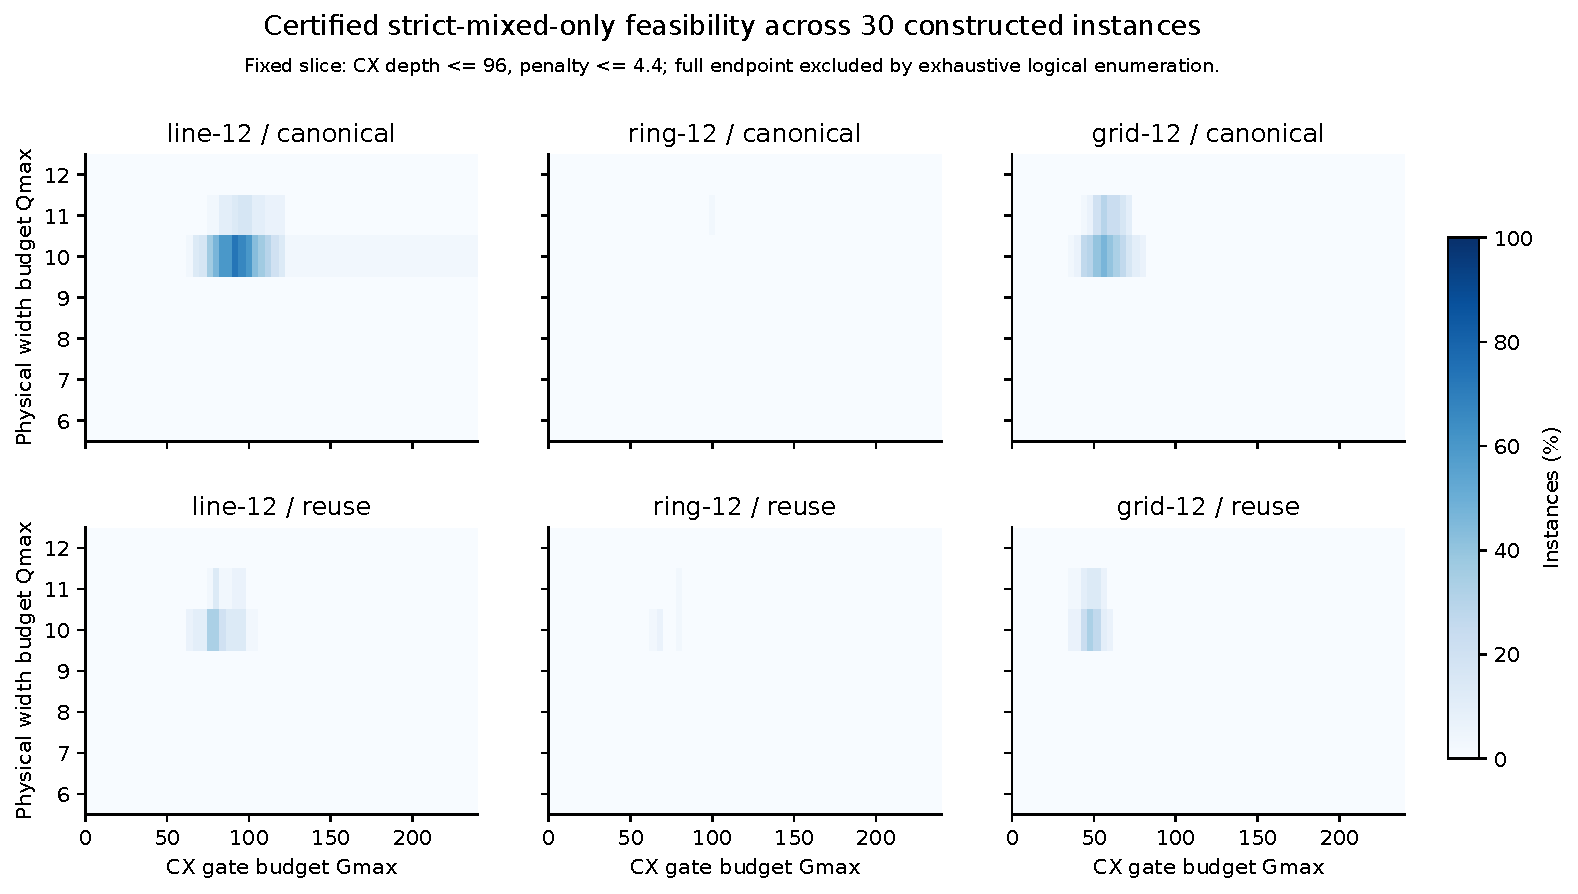
\includegraphics[width=\textwidth]{figures/joint_budget_certified_frequency.pdf}

\caption{Certified mixed-only incidence across the 30 constructed mechanism instances in the fixed $(D_{\max},M_{\max})=(96,4.4)$ slice. Each plotted cell counts independent instances, with the native and full endpoints excluded as specified in Section~\ref{sec:fresh-compiled}. Budget cells and compiler settings are not independent samples.}\label{fig:certified-population}\end{figure}
\section{Additional Experimental Protocol Details}
\label{app:experimental-details}

\subsection{Benchmark definitions and structural coordinates}
\label{sec:applications}

We use weighted Max-3SAT and cubic spin glasses to study how selective
reduction trades interaction locality against auxiliary variables and compiled
resources. Max-3SAT supplies clause-derived signs and overlap; spin glasses
allow sparsity and pair reuse to be varied directly.

\subsubsection{Max-3SAT}

Consider a clause $C=(\ell_i\lor\ell_j\lor\ell_k)$. Define the false-literal indicator
\begin{equation}
    u_{\ell_r}(x_r)
    :=\begin{cases}
       1-x_r, & \ell_r=x_r,\\
       x_r, & \ell_r=\neg x_r.
    \end{cases}
    \label{eq:false-indicator}
\end{equation}
The clause-violation penalty is
\begin{equation}
    P_C(\bm x)=u_{\ell_i}(x_i)u_{\ell_j}(x_j)u_{\ell_k}(x_k),
    \label{eq:clause-penalty}
\end{equation}
which equals one exactly when the clause is violated. A weighted Max-3SAT
instance with $w_C>0$ therefore yields the cubic PUBO~\cite{Nagies2025,Nusslein2023}
\begin{equation}
    f_{\mathrm{3SAT}}(\bm x)=\sum_{C}w_CP_C(\bm x).
    \label{eq:max3sat-pubo}
\end{equation}
After expansion and coefficient aggregation, cubic terms that share a variable
pair can use the same auxiliary. Cancellation must be accounted for before
selecting substitutions and setting penalties; the expansion for arbitrary
literal signs is given in Appendix~\ref{app:max3sat}.

\paragraph{A small worked example}
\label{sec:max3sat-worked-example}

Consider the five-variable weighted instance
\begin{equation}
 f_{\mathrm{3SAT}}^{\mathrm{ex}}(\bm x)
 =g(\bm x)+5x_1x_2x_3-4x_2x_3x_4+2x_1x_4x_5,
 \label{eq:max3sat-worked-expanded}
\end{equation}
where $g(\bm x)=4-4(x_2+x_3+x_4)+4(x_2x_3+x_2x_4+x_3x_4)$.
The clauses and full expansion are given in
Appendix~\ref{app:max3sat-worked}.
The first two cubic terms share $\{2,3\}$. Substituting $y_{23}=x_2x_3$
gives the aggregate residual $A_{23}=5x_1-4x_4$, so
\cref{prop:cubic-mixed-sign} gives the sharp threshold
$M_{23}^{*}=\max\{5,4\}=5$. Taking $M_{23}=6$ yields
\begin{align}
 F_{\mathrm{sel}}(\bm x,y_{23})
 ={}&g(\bm x)+5x_1y_{23}-4y_{23}x_4+2x_1x_4x_5 \nonumber\\
 &+6\PR(x_2,x_3,y_{23}).
 \label{eq:max3sat-worked-selective}
\end{align}
The native representation retains all three cubic terms. Full quadratization
also substitutes $y_{14}=x_1x_4$ in the remaining term, with threshold
$M_{14}^{*}=2$ and penalty $M_{14}=3$. All three representations preserve
the original objective under auxiliary minimisation, as verified in
Appendix~\ref{app:max3sat-worked}.
\Cref{tab:max3sat-worked-comparison} shows the trade-off: the selective choice
removes two cubic terms using one auxiliary, while saving one auxiliary and
four quadratic couplings relative to full reduction. These logical counts do
not establish a compiled-resource or QAOA advantage; those are tested separately.

\begin{table}[t]
    \centering
    \small
    \caption{Logical comparison for the worked Max-3SAT instance. Quadratic
    couplings count distinct degree-two monomials after aggregation.}
    \label{tab:max3sat-worked-comparison}
    \begin{tabular}{@{}lccccc@{}}
        \toprule
        Encoding
        & \shortstack{Total\\variables}
        & \shortstack{Auxiliary\\variables}
        & \shortstack{Retained\\cubic terms}
        & \shortstack{Quadratic\\couplings}
        & Penalties\\
        \midrule
        All-native & $5$ & $0$ & $3$ & $3$  & --\\
        Selective  & $6$ & $1$ & $1$ & $7$  & $M_{23}=6$\\
        Fully quadratized & $7$ & $2$ & $0$ & $11$
            & $M_{23}=6,\ M_{14}=3$\\
        \bottomrule
    \end{tabular}
\end{table}

\subsubsection{Cubic spin glasses}

Higher-order spin-glass models provide a complementary benchmark
\cite{Basso2022,PelofskeShortDepth2024,Pelofske2024}.
For $s_i\in\{-1,+1\}$, write
\begin{equation}
 E(\bm s)=c+\sum_i h_is_i+\sum_{i<j}J_{ij}s_is_j
 +\sum_{i<j<k}K_{ijk}s_is_js_k.
 \label{eq:cubic-spin}
\end{equation}
The main study uses the pure cubic case $c=h_i=J_{ij}=0$.
Substituting $s_i=1-2x_i$ gives a PUBO of degree at most three.
Appendix~\ref{app:spin-glass} specifies the conversion and common rescaling
convention. Varying the cubic supports provides different opportunities for
pair reuse without deriving the interactions from clauses. The two families
are contrasting tests, not a controlled separation of application effects
from hypergraph effects.

\subsubsection{Structural coordinates and benchmark scope}
Analytical QAOA guarantees for regular MaxCut graphs~\cite{Wurtz2021}
and high-depth analyses on large-girth graphs and
hypergraphs~\cite{BassoHighDepth2022} concern specified graph families
and limiting regimes. The finite benchmark ensembles below serve a
different purpose: measuring paired resource and optimisation changes
under exact representation choices.

\label{sec:benchmark-generation}

The main structural axes are cubic sparsity, potential auxiliary reuse, and
hardware connectivity. Coefficient signs affect the penalty through
\cref{eq:cubic-threshold}, but sign balance is recorded as a diagnostic rather
than varied as an additional main axis.

All clauses or hyperedges are expanded and equal monomials are aggregated
before structural features are calculated.  Let $\mathcal C_3(f)$ denote the
remaining nonzero cubic supports and $m_3=|\mathcal C_3(f)|$.  We record the
canonical cubic density $m_3/\binom{n}{3}$ and the load $m_3/n$.  The pair shadow
$\partial_2\mathcal C_3$ is the set of all pairs contained in at least one
cubic support.  Potential pair sharing is summarised by the pair-incidence
score
\begin{equation}
  r_{\mathrm{pair}}
  =1-\frac{|\partial_2\mathcal C_3|}{3m_3},
  \qquad m_3>0,
  \label{eq:pair-reuse-score}
\end{equation}
together with $d(p)=|\{S\in\mathcal C_3(f):p\subseteq S\}|$ and
$\Delta_2=\max_{p\in\partial_2\mathcal C_3}d(p)$.  This score
is zero when every cubic term has three private pairs and increases when pair
incidences are repeated.  It measures potential sharing, not the number of
auxiliaries actually saved by a chosen representation.  When the exact pair
cover is available, the corresponding full-reduction saving is
\begin{equation}
  r_{\mathrm{aux}}
  =1-\frac{\tau_2(\mathcal C_3(f))}{m_3},
  \qquad m_3>0,
  \label{eq:auxiliary-saving-score}
\end{equation}
where $\tau_2$ is the set-cover number defined in \cref{eq:pair-cover}.

Connectivity is assessed by compiling representations of the same instance to
common target graphs. The main targets are all-to-all coupling and a 12-qubit
$3\times4$ grid; additional line, ring, and heavy-hex targets extend the
routing comparison. Capacity failures and common-fit comparisons are handled
by the protocol in Section~\ref{sec:experiments}.

The three workload tiers have different purposes. The oracle tier targets
30 instances per family with $n\in\{5,6,7,8\}$; the QAOA tier targets 36 per
family with $n\in\{6,8,10\}$ and a 12-qubit width limit; the compilation tier
targets 90 per family with $n\in\{8,12,16,20\}$. These generation targets are
distinct from the evaluated subsets reported with each result. The limited
noise subset contains nine instances per family. A separate warm-start study
uses ten instances per family selected using relaxation information only,
without inspecting QAOA outcomes. This strongest-screened set is not pooled
with the original representation comparison. Complete sampling, filtering,
screening, and provenance rules are given in
Appendix~\ref{app:benchmark-generation}.


\subsection{Detailed evaluation protocol}
\label{app:detailed-evaluation-protocol}

We test exactness, compiled resources, and QAOA performance separately. All
comparisons use representations of the same raw instances and a common
execution protocol; full implementation details are given in
Appendices~\ref{app:reproducibility} and~\ref{app:experimental-details}.

\subsubsection{Benchmark scope and comparison rules}
\label{sec:benchmark-tiers}

The oracle tier contains 60 instances for exhaustive exactness and selector
checks, and the compilation tier contains 180 instances for resource
comparisons. The main noiseless QAOA comparison uses 14 test-labelled
instances; the noise and targeted warm-start studies use separate subsets of
18 and 20 instances, respectively. Each set is balanced between the two
families. These evaluated sets are distinct from the generation targets in
Section~\ref{sec:benchmark-generation} and are analysed separately by study.

We compare the native objective, a fully quadratized reference, the selective
design from Section~\ref{sec:selection}, and a matched-random selective
control. Full quadratization uses a minimum-cardinality pair cover with
deterministic tie-breaking. The random control matches only the number of
active pair auxiliaries, not gate count, depth, or penalty size. Five seeded
controls are used; they need not be distinct when the feasible choices are
limited. The exact construction and fallback rules are in
Appendix~\ref{app:experimental-controls}.

Within each family and tier, the recorded training--validation--test split is
$60/20/20$. Settings were chosen using training and validation data, with no
direct selector retuning on test-labelled rows. However, the pool was
available during earlier protocol refinement, so this is an exploratory
study, not a fresh untouched-test evaluation. The broad resource comparison
pools all 180 compilation instances across split labels.

\subsubsection{Exactness and penalty checks}
\label{sec:exactness-protocol}

On each oracle instance we enumerate the original assignments and minimise
over the auxiliary variables, checking
\begin{equation}
 f(\bm x)=\min_{\bm y}F_\rho(\bm x,\bm y)
 \quad\text{for every }\bm x.
 \label{eq:experimental-pointwise-check}
\end{equation}
The main experiments use $M_p=T_p+1$ and check that the minimising auxiliary
assignment is unique and consistent. Tightness checks use $T_p-1$, $T_p$,
and $T_p+1$, recording mismatches, ties, inconsistent minimisers, and explicit
failure witnesses. Penalty-margin sensitivity runs are reported separately.

\subsubsection{Logical and compiled resources}
\label{sec:resource-protocol}

We record register width, auxiliary count, retained cubic terms, aggregated
quadratic couplings, maximum penalty, and coefficient dynamic range. Every
representation uses the same synthesis and compiler settings and the same
five transpiler seeds on all-to-all coupling and the 12-qubit $3\times4$
grid. The compiled metrics are two-qubit gate count, two-qubit depth, and
routing overhead, including inserted SWAPs.

A width failure is recorded separately, not assigned an artificial gate count.
Direct comparisons use instances on which all representations in that
comparison fit the same device. The connectivity extension compares only
selective and matched-random designs on a 12-qubit line, a 12-qubit ring,
and a 19-qubit heavy-hex graph, without rerunning QAOA. Software, coupling
maps, and seeds are specified in Appendix~\ref{app:reproducibility}.

\subsubsection{Relaxation, selection, and warm starts}
\label{sec:experimental-relaxation}

We solve a sparse RLT-style, strengthened recursive-McCormick LP for the
original cubic objective. It uses single, pair, and supported triple
pseudo-moments in $[0,1]$; only the single and pair coordinates are exported
for selection and warm starts. Cubic terms are represented directly in the
LP, without Rosenberg penalties. The complete constraints and solver rules
are given in Appendix~\ref{app:experimental-lp}.

The selector uses the settings in \cref{tab:selector-settings}. In these
experiments, selection and oracle certification use the exact all-to-all
reference synthesis of Appendix~\ref{app:reference-compiler}.
Device-transpiled resources are evaluated subsequently for the selected
representations. Complete
enumeration and branch-and-bound certification are run on the 60 oracle
instances. A separate sensitivity study varies selector settings on that tier,
without rerunning QAOA; details are in Appendix~\ref{app:experimental-sensitivity}.

\begin{table}[t]
\centering
\small
\caption{Main selector settings. The resource order is auxiliary count,
two-qubit gates, two-qubit depth, and maximum penalty. The broader compilation
tier does not impose the 12-qubit QAOA width limit.}
\label{tab:selector-settings}
\begin{tabular}{@{}p{0.39\linewidth}p{0.56\linewidth}@{}}
\toprule
Setting & Value\\
\midrule
Resource weights & $(0.05,0.45,0.45,0.05)$\\
Normalisation scales & $(6,128,96,64)$\\
QAOA-scope limits & 12 qubits; 256 two-qubit gates per cost layer;
 two-qubit depth 192; maximum penalty 128\\
Selector fibre-diagnostic threshold & $0.02$\\
Beam width; main penalty margin & $64$; $1$\\
Warm-start clipping & $\delta=0.05$\\
\bottomrule
\end{tabular}
\end{table}

Warm-start comparisons use cold start, original-only warming, and
original-plus-auxiliary warming with either pair moments or the independence
approximation. The corresponding probabilities and matched mixers follow
Section~\ref{sec:warm-start}; the experimental policies are specified in
Appendix~\ref{app:experimental-warm}.

The original warm-start runs (E4) use the first LP optimum returned by HiGHS.
The selector and targeted warm-start study instead use a deterministic
secondary optimisation to choose an optimum-face representative. These rules
can yield different pseudo-moments for the same instance. The 20 targeted
instances were screened using relaxation information only, not QAOA outcomes.
They form a strongest-screened subset, not a representative random sample,
and are analysed separately from the original E4 runs. The coordinate
correction restores the archived probability vectors and fixed designs for
both studies, without solving the LP again or screening new instances;
its execution and validation are described in
Appendix~\ref{app:warmstart-correction-provenance}.

\subsubsection{QAOA budgets and optimisation objective}
\label{sec:qaoa-evaluation}

Each representation is optimised independently using COBYLA, with three
restarts and at most 60 objective evaluations per restart. The loss is the
original-objective expectation $\mathcal E_f$, obtained by ignoring the
auxiliary register. Encoded energy and auxiliary consistency are diagnostics,
not terms in this classical loss.

Equal-layer comparisons use $p\in\{1,2\}$. For a two-qubit-gate budget
$B\in\{128,256\}$, let $g_\sigma$ be the median one-layer two-qubit gate
count on the grid over the five transpiler seeds. For $g_\sigma>0$, the
assigned depth is
\begin{equation}
 p_\sigma(B)=\left\lfloor\frac{B}{g_\sigma}\right\rfloor,
 \qquad p_\sigma(B)g_\sigma\leq B.
 \label{eq:qaoa-gate-budget-depth}
\end{equation}
If $g_\sigma>B$, the stored $p=0$ row is an initial-state baseline with no
trainable parameters. In particular, the 128-gate comparison includes such
rows; their counts and the subset on which every design fits at least one
layer are reported separately. The targeted warm-start study uses only
$p=1,2$ and contains no zero-layer rows.

\subsubsection{Aggregation, uncertainty, and supplementary analyses}
\label{sec:structure-noise-protocol}

The raw instance is the statistical unit. For resources, we take the median
over transpiler seeds for each design, then average the five random-control
design values within each instance. For QAOA, we average the three restart
scores per design, then the five random-control design means. No best-seed,
best-restart, or best-random-design selection is used. Paired differences are
formed only after these within-instance aggregations.

Resource comparisons report medians of paired instance differences. QAOA,
warm-start, and noise comparisons report means and two-sided 95\%
Student-$t$ intervals across instances. The corrected warm-start intervals
use $n-1$ degrees of freedom, are unadjusted for multiple comparisons,
and are exploratory; an interval containing zero does not establish
equivalence or absence of an effect. Repeated seeds and restarts are not
additional independent samples. The exploratory regime labels use a separate
within-endpoint stability rule, not population-level confidence intervals;
its thresholds are in Appendix~\ref{app:experimental-statistics}.

Noiseless statevector results are the primary QAOA comparison. The limited
noise study uses 18 structurally selected instances on the grid, with
representative depolarising and readout errors rather than a calibrated real
device. Parameters are optimised noiselessly and reused at both noise levels
without re-optimisation. Full noise, shot, and seed settings remain in
Appendix~\ref{app:reproducibility}. The structural study uses the sparsity,
pair-reuse, and connectivity axes of Section~\ref{sec:benchmark-generation}.
All these analyses are exploratory; intervals describe uncertainty, and
unadjusted multiple-setting $p$-values are not used to claim significance.



This appendix contains the implementation details supporting
Section~\ref{sec:experiments}. Appendix~\ref{app:reproducibility} retains
software versions, compiler configuration, generation records, optimiser
seeds, and noise settings.

\subsection{Fully reduced and matched-random references}
\label{app:experimental-controls}

The historical full-quadratization baseline uses a minimum-cardinality pair cover of all
cubic supports.  Ties are resolved by the lexicographically smallest active
pair set and then by a lexicographic term-to-pair assignment.  This fixes the
auxiliary count and penalty profile rather than leaving ``full'' as an
unspecified quadratization.

The matched-random control is matched only on the number of active pair
auxiliaries.  Five feasible controls are generated from the fixed seeds
$2026082711$--$2026082715$.  A seeded candidate pair set is followed by a
deterministic augmenting-path assignment of reduced terms.  After 256 failed
pair-set attempts, the selected pair set is reused with a random valid
assignment; if no distinct control exists, the selected design is retained.
When the selected design is native, its matched control is therefore native as
well.  All derived representations retain the raw instance identifier so that
reported contrasts can be paired.


\subsection{Relaxation and optimum-face selection}
\label{app:experimental-lp}

The implementation records its relaxation as \texttt{SA\_RLT\_level\_2}.
Because conventions for hierarchy levels differ, we define the exact model
used here.  It is a sparse RLT-style~\cite{SheraliAdams1990}, strengthened
recursive-McCormick~\cite{McCormick1976} relaxation of the canonical
cubic objective
\begin{equation}
  f(\bm x)=c_{\varnothing}
  +\sum_i c_i x_i
  +\sum_{i<j}c_{ij}x_ix_j
  +\sum_{i<j<k}c_{ijk}x_ix_jx_k.
  \label{eq:experimental-rlt-canonical}
\end{equation}
Let $\mathcal T:=\{(i,j,k):i<j<k,\ c_{ijk}\neq0\}$.  The LP has one
single-variable pseudo-moment $\widehat\mu_i$ for every original variable, one
pair pseudo-moment $\widehat q_{ij}$ for every $i<j$, and one triple
pseudo-moment $\widehat t_{ijk}$ for every $(i,j,k)\in\mathcal T$.  All are
bounded in $[0,1]$, and the primary objective is
\begin{equation}
  \min_{\widehat\mu,\widehat q,\widehat t}
  \left(
    \sum_i c_i\widehat\mu_i
    +\sum_{i<j}c_{ij}\widehat q_{ij}
    +\sum_{(i,j,k)\in\mathcal T}c_{ijk}\widehat t_{ijk}
  \right).
  \label{eq:experimental-rlt-objective}
\end{equation}
The constant $c_{\varnothing}$ is added back only when the objective value is
reported.  Cubic terms are represented directly by $\widehat t_{ijk}$; no
Rosenberg penalty is used inside this relaxation.

For every $i<j$, the pair envelope is
\begin{equation}
  \widehat q_{ij}\leq\widehat\mu_i,
  \quad
  \widehat q_{ij}\leq\widehat\mu_j,
  \quad
  \widehat q_{ij}\geq\widehat\mu_i+\widehat\mu_j-1.
  \label{eq:experimental-rlt-pair}
\end{equation}
For each $(i,j,k)\in\mathcal T$, the triple variable obeys
\begin{equation}
  \widehat t_{ijk}\leq
  \widehat\mu_i,\widehat\mu_j,\widehat\mu_k,
  \qquad
  \widehat t_{ijk}\geq
  \widehat\mu_i+\widehat\mu_j+\widehat\mu_k-2,
  \label{eq:experimental-rlt-triple-single}
\end{equation}
where the first shorthand denotes three separate upper bounds.  For each
pair--remaining-index decomposition
$(ab,c)\in\{(ij,k),(ik,j),(jk,i)\}$, we additionally impose
\begin{equation}
  \widehat t_{ijk}\leq\widehat q_{ab},
  \qquad
  \widehat t_{ijk}\geq\widehat q_{ab}+\widehat\mu_c-1.
  \label{eq:experimental-rlt-triple-pair}
\end{equation}
These constraints recover the intended products at Boolean points.  At a
fractional solution they are relaxation pseudo-moments and need not be the
marginals of one joint probability distribution.

The LP is solved with SciPy 1.18.1 using
\texttt{scipy.optimize.linprog}, the HiGHS method, and presolve.  The v2
selector uses a second solve after obtaining the primary value $z^\star$.  It
keeps the primary objective within
\begin{equation}
  \left|\bm c^\top\bm v-z^\star\right|\leq10^{-9}
  \label{eq:experimental-rlt-optimum-face}
\end{equation}
and minimises a positive secondary objective whose weights are derived
deterministically from SHA-256 labels.  The variable order is all singles,
lexicographic pairs, and then sorted supported triples.  Under the pinned
solver stack, this supplies the selector with a reproducible representative of
the primary optimum face.  The coordinates $\widehat\mu_i$ and
$\widehat q_{ij}$ are read directly from the returned vector and clipped to
$[0,1]$ only to remove small numerical violations; the triple coordinates are
not exported as selector moments.

E4 uses the same feasible LP and primary objective, but its frozen runs use the
first optimal vector returned by HiGHS rather than the selector's secondary
representative.  Therefore, when the primary optimum face is not a single
point, the selector and E4 can use different pseudo-moment vectors.  Before
interpreting the E4 results, we report the distribution of
$|\widehat\mu_i-1/2|$; instances whose values are almost uniform carry little
warm-start information and are identified as such.


\subsection{Certification and selector sensitivity}
\label{app:experimental-sensitivity}

The main selector settings are listed in \cref{tab:selector-settings}; final
score ties are broken lexicographically.

For the 60 oracle-tier instances, we also ran the best-bound branch-and-bound
procedure of \cref{alg:app-branch-and-bound}.  At each step, the unresolved
state with the smallest valid lower bound is expanded first, and one trace row
is stored after every 256 explored nodes.  A run is declared complete only
when the frontier is resolved, the final lower and upper bounds are equal, and
the selected value matches the previously frozen complete-enumeration optimum.
The compiler contribution in a partial state uses the valid but conservative
lower bound of zero.  These runs therefore check the certificate
implementation on small finite search spaces; they are not a claim about
large-instance scaling.


We performed a one-factor-at-a-time sensitivity study on the same 60 oracle
instances.  Starting from weights $(0.05,0.45,0.45,0.05)$, beam width 64,
fibre threshold 0.02, and penalty margin 1.0, we varied the resource weights,
tested gate-only, depth-only, and joint gate--depth scores, used beam widths
16, 32, and 128, changed the fibre threshold to $0$, $0.01$, $0.05$, and
$0.10$, and changed the penalty margin to $0.5$ and $2.0$.  We also included
a deterministic greedy baseline and a deterministic maximum-pair-reuse
baseline.  This study compares representation choices and resource outputs
only; it does not rerun QAOA.


\subsection{Warm-start policies}
\label{app:experimental-warm}

The warm-start comparison uses clipping value $\delta=0.05$ and compares four policies including cold start. From the relevant LP vector we set
\begin{equation}
  p_i=\operatorname{clip}_\delta(\widehat\mu_i),
  \qquad
  p_{ij}^{\mathrm{pair}}
  =\operatorname{clip}_\delta(\widehat q_{ij}),
  \qquad
  p_{ij}^{\mathrm{ind}}=p_i p_j.
  \label{eq:experimental-warm-probabilities}
\end{equation}
Cold start puts every qubit in $|+\rangle$ and uses the usual $X$ mixer.
Original-only warm start uses $p_i$ and its matched mixer on the original
qubits, while each auxiliary remains at probability $1/2$ with an $X$ mixer.
The original-plus-auxiliary policy also applies a matched mixer to the
auxiliaries, using $p_{ij}^{\mathrm{pair}}$ as the main rule.  The product of
the individually clipped probabilities, $p_{ij}^{\mathrm{ind}}$, is the single
auxiliary ablation, without further clipping. The LP supplies pair coordinates
in these experiments, so this ablation deliberately omits available pair
information.

\paragraph{Null control at fixed optimiser coordinates.}
The cold single-qubit unitary is $e^{-i\beta X}$. With
$B(\omega)=2\sqrt{\omega(1-\omega)}X+(1-2\omega)Z=-h_M(\omega)$,
the implemented warm gate is $e^{-i\beta B(\omega)}$ on every warmed
qubit. Setting \emph{all} original and auxiliary probabilities to $1/2$
therefore gives the same statevector, probabilities, and metrics as cold
start at each parameter vector. The regression covers $p=1,2$, native and
auxiliary designs, and all four policy paths. Setting only the original
probabilities to $1/2$ is insufficient: the independence rule would set an
auxiliary probability to $1/4$. The control explicitly overrides the full
register after policy construction.

\paragraph{Targeted warm-start addendum.}
The 20 strongest-screened instances are evaluated at equal layer depths
$p=1$ and $p=2$.  Every selected representation has at least one active
auxiliary, and no zero-layer bookkeeping row is included.  We compare cold
start, original-variable-only warm start, original-and-auxiliary warm start
using the pair pseudo-moments, and the independence closure
$p_{ij}=p_i p_j$.  Each setting uses three COBYLA restarts and 60 objective
evaluations per restart, giving 480 run rows in total.  All runs use noiseless
statevector evaluation. The archived addendum probabilities were obtained
with the deterministic secondary optimum-face selection used by the v2
selector, whereas the original E4 probabilities came from the first primary
optimum. The correction restores both archived probability sets and reruns
all 480 targeted tasks; it does not invoke either LP selection procedure.


\subsection{Secondary statistics and regime labels}
\label{app:experimental-statistics}

For paired instance differences $d_i$, let $\bar d$ denote their mean.
A paired standardised effect is reported as
$d_z=\bar d/s_d$, where $s_d$ is the sample standard deviation of the paired
instance differences.  Win/tie/loss counts use the same raw instances and the
declared equivalence band.  The E5 endpoint classification retains its frozen
paired normal interval over repeated observations within each endpoint and is used only for the
exploratory regime counts.  The regime study uses frozen
equivalence bands of 5\% for gate count, depth, and routing overhead, and 0.01
objective units for the QAOA score.  A result is called helpful or detrimental
only when its paired interval lies beyond the corresponding band; otherwise it
is assigned to the residual (inconclusive) category. This category includes
intervals overlapping the band and does not establish practical equivalence.

These endpoint intervals describe algorithmic stability, not across-instance
uncertainty. Sign balance and coefficient heterogeneity remain diagnostics,
not additional factorial axes.


\FloatBarrier
\section{Supplementary Numerical Results}
\label{app:supplementary-results}

These results supplement the four comparisons in Section~\ref{sec:results}.
Protocols and within-instance aggregation follow Section~\ref{sec:experiments}
and Appendices~\ref{app:reproducibility}--\ref{app:experimental-details}.

\FloatBarrier
\subsection{Complete exactness counts}
\label{app:results-exactness}

We first checked the reduction by exhaustive enumeration on 60 small
instances, with 30 Max-3SAT instances and 30 cubic spin-glass instances.  The
selected designs were not all the same: 30 were all-native, 23 were strictly
mixed, and seven were fully reduced.  These instances contain 5,696 distinct
instance--original-assignment pairs.  Across 1,384 representation, design,
penalty, and target-pair trials, the verifier repeatedly enumerated the same
assignments where required, giving 124,672 original-assignment evaluations and
585,408 joint original--auxiliary evaluations in total.  These totals measure
the full verification workload rather than the number of distinct original
assignments.

Section~\ref{sec:results-exactness} summarises the threshold behaviour.
Table~\ref{tab:e1-exactness-summary} reports the counts:
5,351 at-threshold inconsistent ties, 5,639 below-threshold mismatches,
and 452 saved failure witnesses, all with non-zero error.

\begin{table}[!htbp]
    \centering
    \small
    \caption{Summary of the exhaustive exactness checks.  The
    above-threshold setting produced no mismatch or inconsistent minimiser in
    any tested case.}
    \label{tab:e1-exactness-summary}
    \begin{tabular}{@{}lrrr@{}}
        \toprule
        Family and representation
        & \shortstack{At-threshold\\ties}
        & \shortstack{Below-threshold\\mismatch}
        & \shortstack{Saved below-threshold\\witnesses}\\
        \midrule
        Cubic spin glass, fully reduced & 970 & 970 & 78\\
        Max-3SAT, fully reduced          & 268 & 268 & 62\\
        Max-3SAT, selective              & 311 & 315 & 52\\
        Max-3SAT, matched random         & 3,802 & 4,086 & 260\\
        \midrule
        Total                            & 5,351 & 5,639 & 452\\
        \bottomrule
    \end{tabular}
\end{table}


\FloatBarrier
\subsection{Selector validation, certification, and sensitivity}
\label{app:results-selector}

\begin{table}[!htbp]
    \centering
    \small
    \caption{Work and runtime for the oracle-tier methods in
    \cref{tab:selector-oracle-validation}. Entries are medians [interquartile
    ranges]; timings describe the machine used in this study.}
    \label{tab:selector-oracle-work}
    \begin{tabular}{@{}lrr@{}}
        \toprule
        Method & Candidate evaluations & Runtime (s)\\
        \midrule
        Complete enumeration & 4096 [1024, 16384] & 1.274 [0.370, 6.112]\\
        Pareto beam & 640 [448, 832] & 0.832 [0.603, 1.158]\\
        Greedy native-completion & 19 [16, 22] & 0.00525 [0.00414, 0.00667]\\
        \bottomrule
    \end{tabular}
\end{table}

\Cref{fig:selector-oracle-summary} gives the graphical counterpart of
\cref{tab:selector-oracle-validation}. Certification timings and stored gap
traces are given in \cref{tab:selector-bnb-certification,fig:selector-bnb-gap}.

\begin{figure}[!htbp]
    \centering
    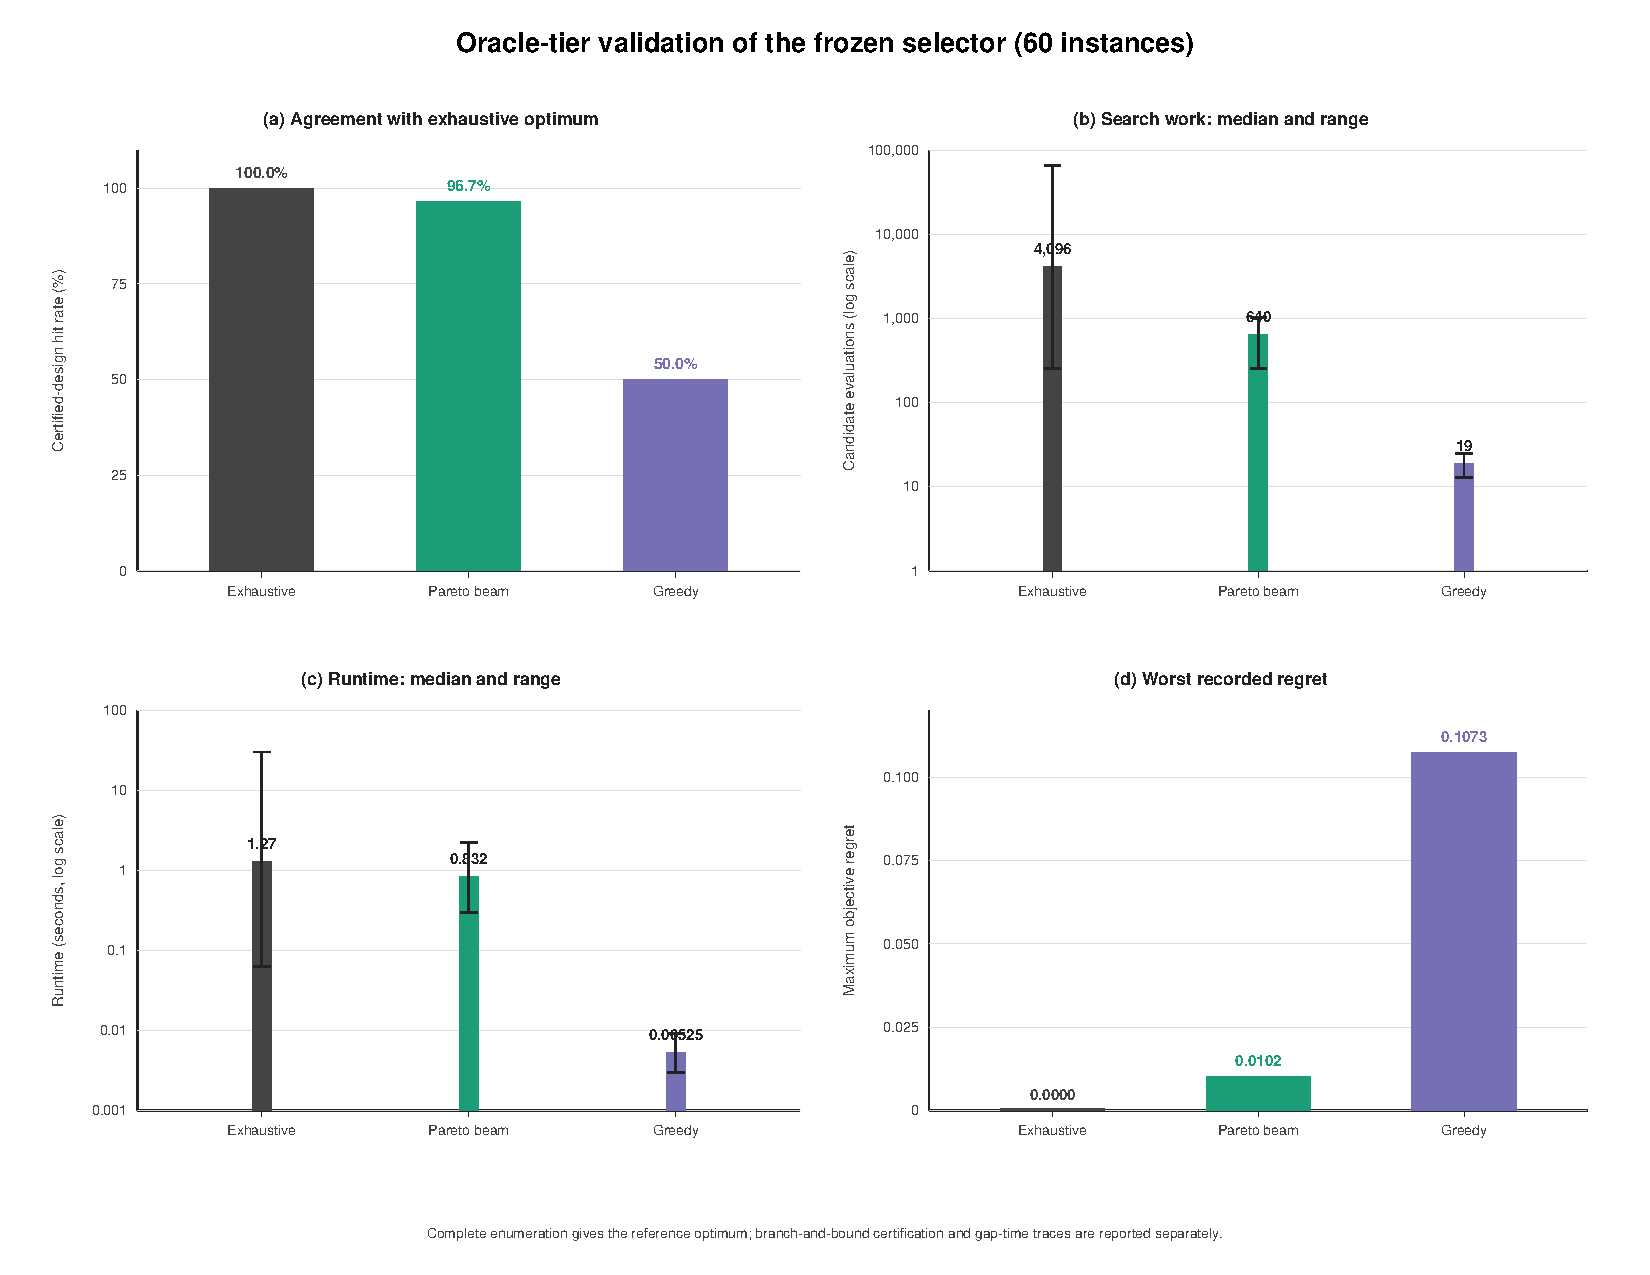
\includegraphics[width=\textwidth]{figures/figure_oracle_selector_summary.pdf}
    \caption{Numerical oracle-tier selector check using the frozen results.
    Complete enumeration supplies the reference optimum, and the practical
    methods are compared with it using hits, work, runtime, and regret.
    Branch-and-bound certification and gap traces are reported separately in
    \cref{tab:selector-bnb-certification,fig:selector-bnb-gap}.}
    \label{fig:selector-oracle-summary}
\end{figure}

\begin{table}[!htbp]
    \centering
    \small
    \caption{Branch-and-bound certification on the oracle tier.  Runtime is
    descriptive for the machine used in this study.}
    \label{tab:selector-bnb-certification}
    \resizebox{\linewidth}{!}{%
\begin{tabular}{@{}lrrrrrr@{}}
        \toprule
        Family & Certified
        & Median nodes & Max. nodes
        & Median time (s) & Max. time (s)
        & Max. final gap\\
        \midrule
        Cubic spin glass & 30/30 & 5,461 & 33,462 & 2.469 & 14.715 & 0\\
        Max-3SAT         & 30/30 & 5,461 & 55,453 & 2.336 & 26.526 & 0\\
        \bottomrule
    \end{tabular}}%

\end{table}

The repaired certifier permits an initially absent incumbent and returns
interrupted frontier bounds for the implemented feasible set. The experiments
freeze the stored floating-point raw moments and accept a design when
$\widehat E_{\mathrm{fib}}^{\mathrm{computed}}\leq\tau_{\mathrm{fib}}+10^{-9}$,
in addition to the declared resource constraints. Scores and reference-resource
bounds use rational arithmetic. Numerical certification therefore concerns
this deterministic, tolerance-defined feasible set, not the exact LP moments
or the zero-tolerance feasible set in the mathematical definition in Section~\ref{sec:selection}.
All 60 completed historical traces remain valid under the repaired interface.

\begin{figure}[!htbp]
    \centering
    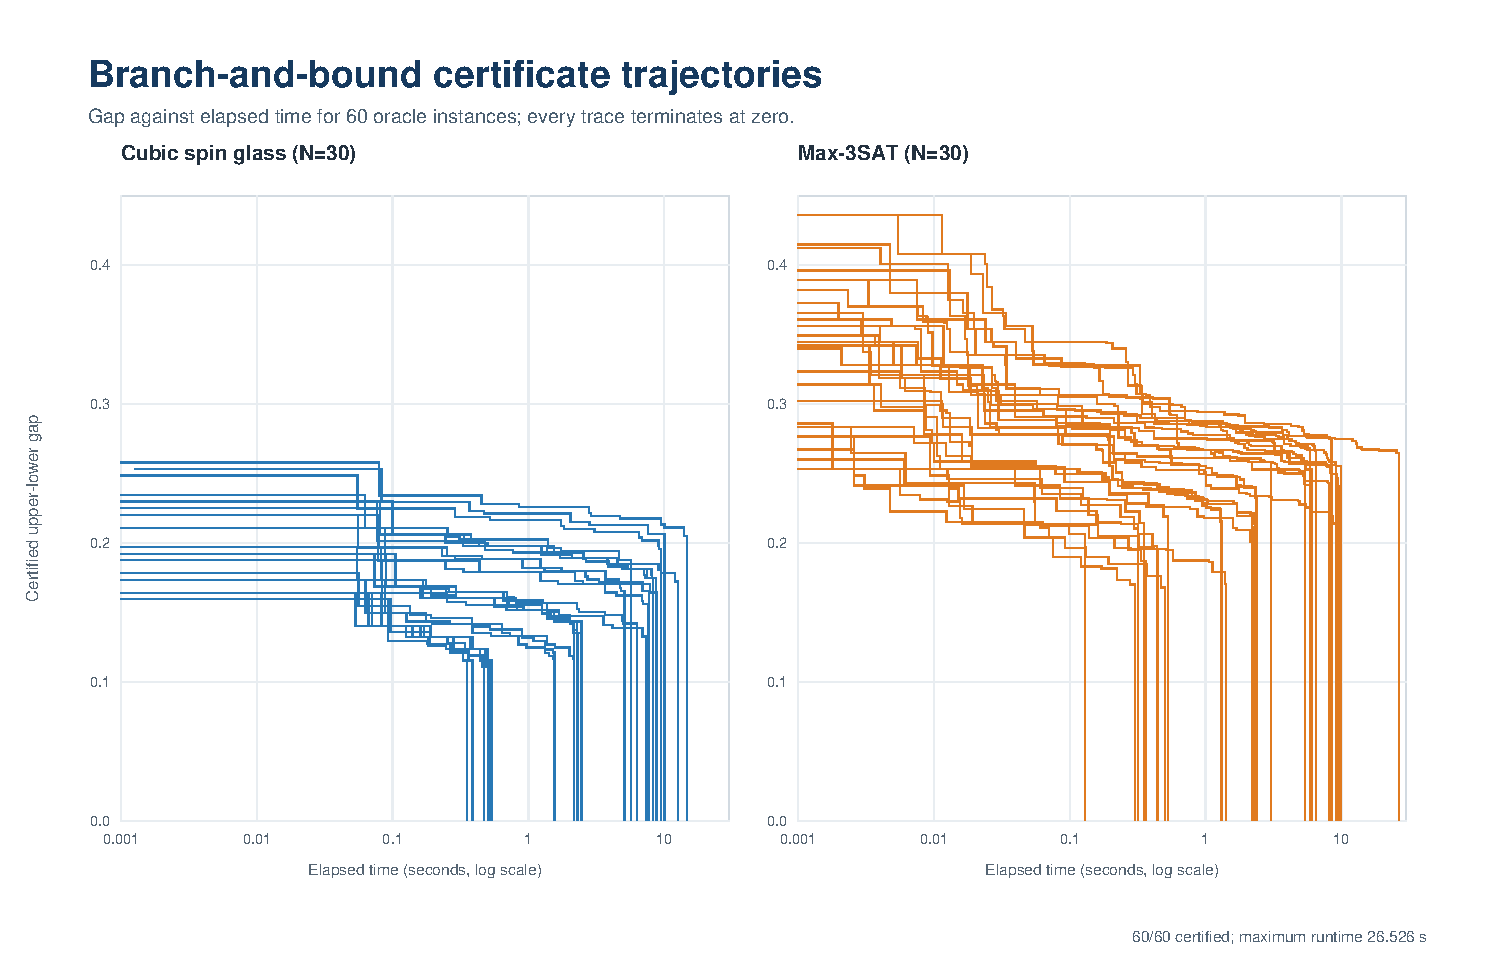
\includegraphics[width=\textwidth]
    {figures/figure_certification_gap_time.pdf}
    \caption{Stored certificate gap against elapsed time for the 60 oracle
    instances: (a) spin glass and (b) Max-3SAT. Each trace terminates at zero.  The figure checks the small
    certification cases and is not used as a scaling claim.}
    \label{fig:selector-bnb-gap}
\end{figure}

\begin{table}[!htbp]
    \centering
    \small
    \caption{Guardrail on/off ablation on the 48 training and validation
    calibration instances.  Fibre-risk medians and score changes use only the
    instances whose selected design changed.  Here
    $\Delta S=S_{\mathrm{guarded}}-S_{\mathrm{unguarded}}$.}
    \label{tab:selector-guardrail-ablation}
    \resizebox{\textwidth}{!}{%
    \begin{tabular}{@{}lrrrrrr@{}}
        \toprule
        Split & $n$ & Changed
        & \shortstack{Violations\\off $\rightarrow$ on}
        & \shortstack{Median fibre risk\\off $\rightarrow$ on}
        & Median $\Delta S$ & Max.\ $\Delta S$\\
        \midrule
        Train      & 36 & 10 & $10\rightarrow0$
                   & $0.03142\rightarrow0.01820$ & 0.01654 & 0.03802\\
        Validation & 12 &  2 & $2\rightarrow0$
                   & $0.03301\rightarrow0.01753$ & 0.03451 & 0.04870\\
        Combined   & 48 & 12 & $12\rightarrow0$
                   & $0.03142\rightarrow0.01820$ & 0.01849 & 0.04870\\
        \bottomrule
    \end{tabular}%
    }
\end{table}

Without the guardrail, 12 of 48 calibration choices exceeded the threshold.
Enabling it changed exactly these choices and removed all recorded violations,
at a median resource-score increase of $0.01849$ among changed cases. All
changes were in Max-3SAT. This is a training/validation calibration ablation.
The separate one-factor-at-a-time study covers all 60 oracle instances.

\begin{table}[!htbp]
    \centering
    \small
    \caption{One-factor-at-a-time selector sensitivity on 60 oracle
    instances.  ``Changed'' counts representations different from the main
    setting.  Every row uses the same raw instances.}
    \label{tab:selector-sensitivity-addendum}
    \resizebox{\textwidth}{!}{%
    \begin{tabular}{@{}llrr@{}}
        \toprule
        Block & Alternative values & Changed choices & Feasible runs\\
        \midrule
        Resource weights
        & equal, auxiliary-heavy, penalty-heavy
        & 30, 30, 27 & 60/60 each\\
        Resource mode
        & gate-only, depth-only, gate--depth
        & 20, 37, 8 & 60/60 each\\
        Beam width
        & 16, 32, 128
        & 5, 2, 1 & 60/60 each\\
        Fibre threshold
        & 0, 0.01, 0.05, 0.10
        & 27, 23, 17, 18 & 60/60 each\\
        Penalty margin
        & 0.5, 2.0
        & 5, 7 & 60/60 each\\
        Greedy baseline
        & deterministic
        & 30 & 60/60\\
        Maximum-reuse baseline
        & deterministic
        & -- & 10/60\\
        \bottomrule
    \end{tabular}%
    }
\end{table}

\begin{figure}[!htbp]
    \centering
    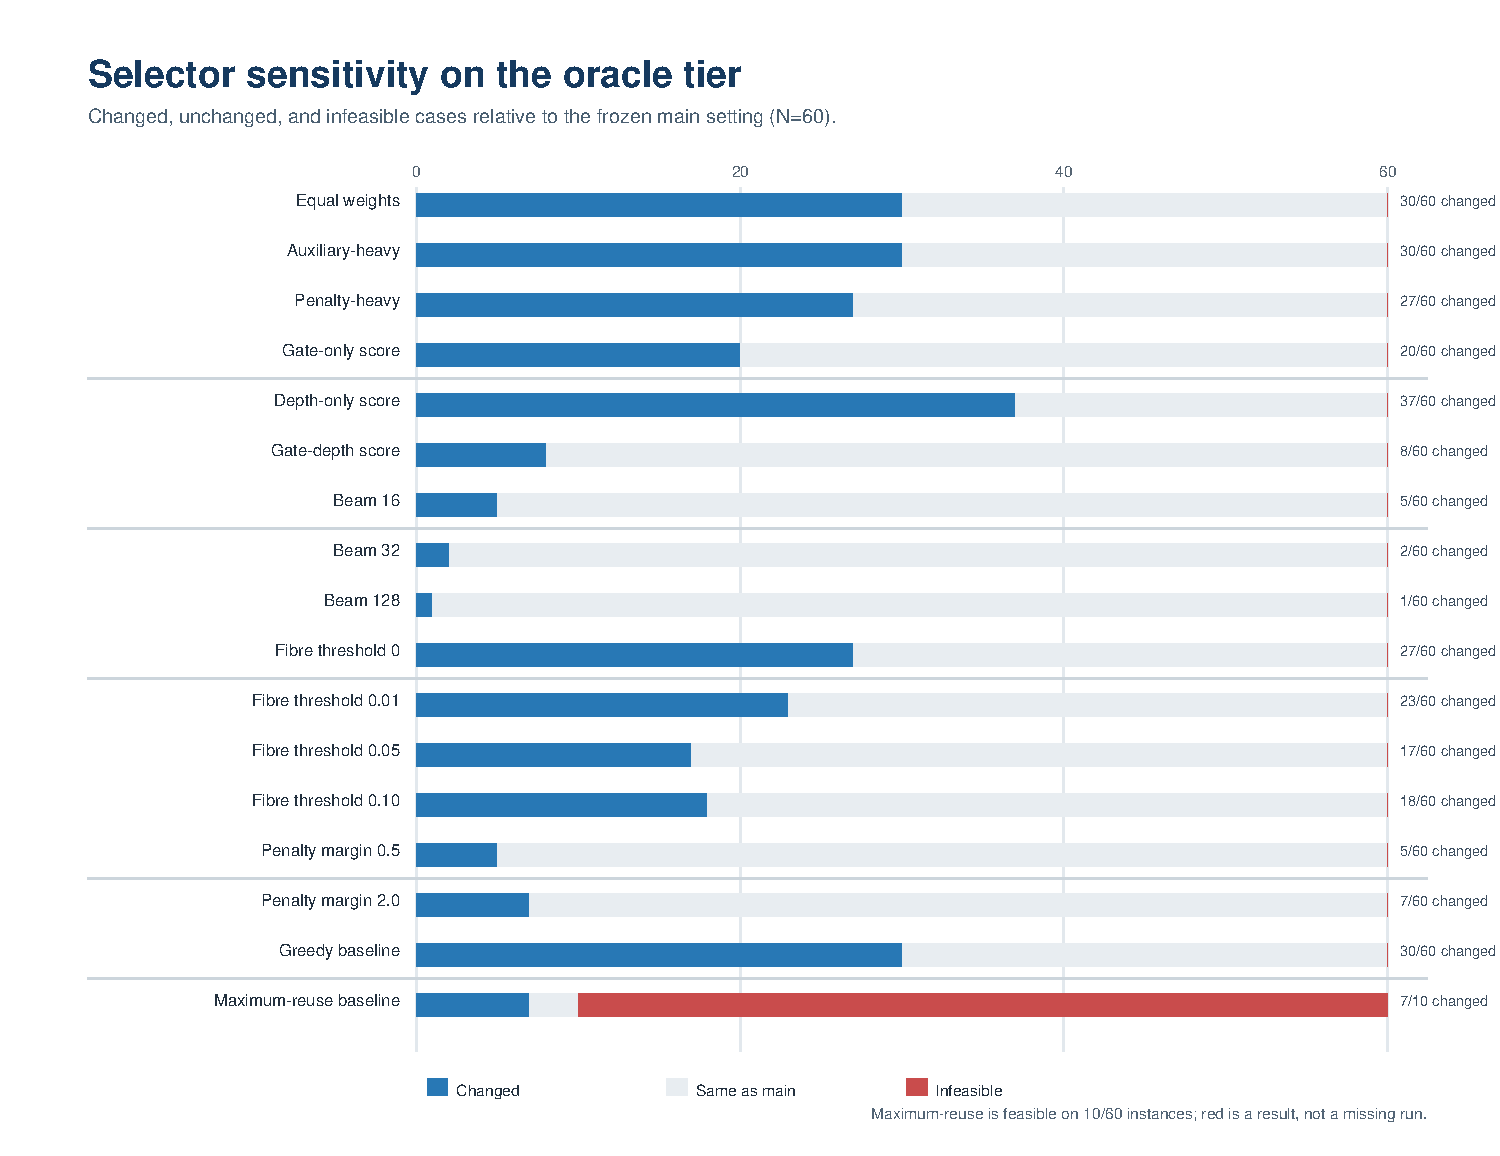
\includegraphics[width=\textwidth]
    {figures/figure_selector_sensitivity_addendum.pdf}
    \caption{Choice stability and feasibility in the selector sensitivity
    study.  A changed choice differs from the frozen main setting.  Red bars
    identify infeasible cases rather than missing runs.}
    \label{fig:selector-sensitivity-addendum}
\end{figure}
The deterministic greedy baseline was feasible in all 60 cases but differed
from the main selector in 30.  The maximum-reuse rule was feasible on only ten
Max-3SAT instances and on none of the spin-glass instances, so it is not a
generally usable replacement for the constrained selector.

The scalar resource score is not compared directly across weight ablations,
because changing the weights also changes the meaning of that score.  We use
the sweep to study choice stability and the underlying gate, depth, auxiliary,
and penalty values, rather than to claim that one alternative weight vector is
universally better.

\subsection{Marginal resource levels and selector diagnostics}
\label{app:results-resources}

The all-to-all tier contains 108 training, 36 validation, and 36 test-labelled
instances. Marginal medians describe resource scale; their differences are
not paired effects. For example, selective and native Max-3SAT gate medians
are 145 and 178, while the median paired difference is $-25$, not $-33$.
On the grid, 4,845 of 7,200 scheduled rows are expected width failures, with
no unexpected compiler failures. Main common-fit results are in
\cref{tab:e2-sparse-common-paired}.

\begin{table}[!htbp]
    \centering
    \small
    \caption{Marginal median logical and compiled resource levels on the
    all-to-all reference topology.  These levels show scale, but the difference
    between two entries is not the within-instance paired effect.}
    \label{tab:e2-all-to-all-resources}
    \begin{tabular}{@{}llrrrr@{}}
        \toprule
        Family & Representation
        & Qubits
        & Auxiliaries
        & \shortstack{Two-qubit\\gates}
        & \shortstack{Two-qubit\\depth}\\
        \midrule
        Max-3SAT & Native          & 12 & 0 & 178 & 119.5\\
                 & Fully reduced   & 18 & 7 & 137 & 46\\
                 & Selective       & 18 & 4 & 145 & 56\\
                 & Matched random  & 18 & 4 & 180 & 94\\
        \addlinespace
        Cubic spin glass & Native         & 12 & 0 & 96  & 79\\
                         & Fully reduced  & 18 & 6 & 148 & 47\\
                         & Selective      & 14 & 1 & 116 & 63.5\\
                         & Matched random & 14 & 1 & 117 & 82\\
        \bottomrule
    \end{tabular}
\end{table}

\begin{table}[!htbp]
    \centering
    \small
    \caption{Median diagnostics for the 90 compilation-tier selective designs
    in each family.  Fibre risk is the normalised raw-moment excess used by the v2
    selector guardrail; the threshold is 0.02.  Time is selector runtime in seconds.}
    \label{tab:e2-selector-diagnostics}
    \resizebox{\textwidth}{!}{%
    \begin{tabular}{@{}lrrrrrrr@{}}
        \toprule
        Family & Retained cubic & $M_{\max}$ & Dynamic range & Fibre risk
        & Score & Compiler calls & Time\\
        \midrule
        Cubic spin glass & 19 & 9  & 5.5 & 0.00115 & 0.7233 & 4096 & 2.19\\
        Max-3SAT         & 6.5 & 12 & 59.5 & 0.01925 & 0.8156 & 4288 & 1.94\\
        \bottomrule
    \end{tabular}%
    }

\end{table}
All 180 compilation-tier selected designs satisfied the raw-moment 0.02
selector guardrail; the
largest stored normalised excess was below 0.02.  The different median retained
cubic counts also show that the repaired v2 selector did not apply the same amount
of reduction to the two families.

We do not report a compilation-tier
certificate gap because these rows are beam-search incumbents and no common
certified lower bound was produced.


\FloatBarrier
\subsection{Additional coupling maps}
\label{app:results-connectivity}

Of 16,200 added compiler rows, 7,020 succeeded and 9,180 were expected width
failures; no unexpected compiler failure was recorded. The table reports
paired medians, while the figure reports means and instance-level intervals.

\begin{table}[!htbp]
    \centering
    \small
    \caption{Selective-minus-matched-random resource differences on the three
    added coupling maps.  Values are paired medians after taking the median
    over transpiler seeds and the mean over matched-random designs within each
    instance.  Negative values favour the selective choice.  Parentheses give
    the number of instances on which selective is strictly lower.}
    \label{tab:e2-additional-topologies}
    \resizebox{\textwidth}{!}{%
    \begin{tabular}{@{}llrrrr@{}}
        \toprule
        Topology & Family & Common $N$
        & $\Delta$ two-qubit gates & $\Delta$ two-qubit depth
        & $\Delta$ routing\\
        \midrule
        Line-12
        & Spin glass & 39 & $0.00$ (8) & $0.00$ (9) & $0.00$ (8)\\
        & Max-3SAT   & 18 & $-38.4$ (18) & $-33.3$ (18) & $-26.0$ (18)\\
        Ring-12
        & Spin glass & 39 & $0.00$ (8) & $0.00$ (9) & $0.00$ (8)\\
        & Max-3SAT   & 18 & $-36.3$ (18) & $-31.8$ (18) & $-26.6$ (18)\\
        Heavy-hex-19
        & Spin glass & 65 & $0.00$ (24) & $0.00$ (26) & $0.00$ (24)\\
        & Max-3SAT   & 55 & $-55.8$ (53) & $-52.4$ (55) & $-35.6$ (52)\\
        \bottomrule
    \end{tabular}%
    }
\end{table}

\begin{figure}[!htbp]
    \centering
    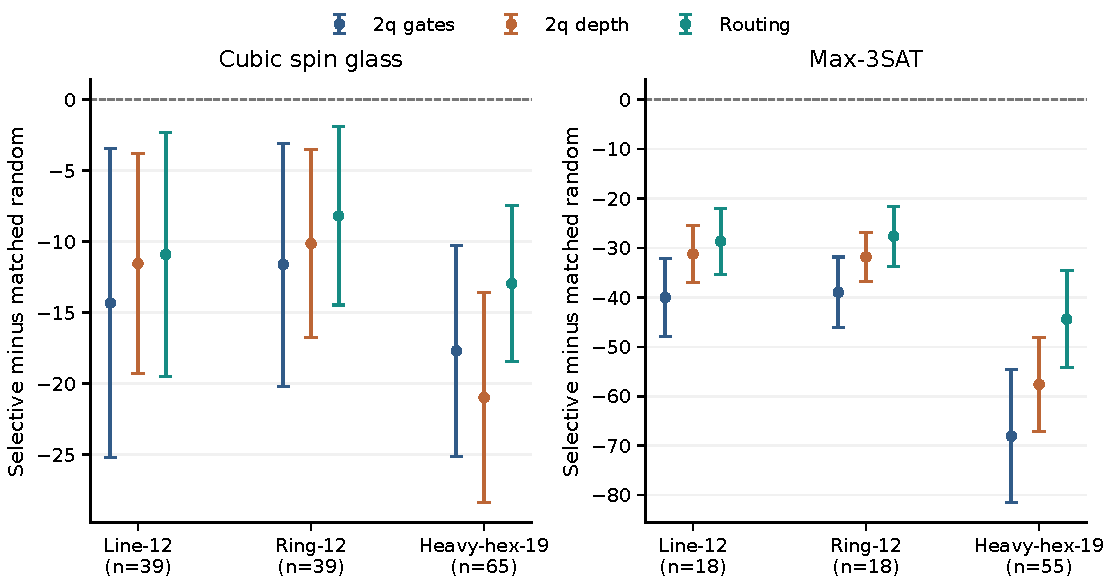
\includegraphics[width=\textwidth]
    {figures/figure_additional_topologies.pdf}
    \caption{Mean paired selective-minus-matched-random resource changes on
    the additional coupling maps: (a) spin glass and (b) Max-3SAT, with 95\% Student-$t$ intervals across raw
    instances.  The comparison uses only instances that fit in both
    representations.  Negative values favour selective reduction; the primary
    medians are reported in \cref{tab:e2-additional-topologies}.}
    \label{fig:e2-additional-topologies}
\end{figure}
Capacity remains part of the result.  The 12-qubit line and ring each had 39
common-fit spin-glass and 18 common-fit Max-3SAT instances, while the
19-qubit heavy-hex graph had 65 and 55.  The corresponding test-labelled
counts were only 7 and 2 on line and ring, and 12 and 9 on heavy-hex.  Since
heavy-hex also has greater capacity, its numerical differences cannot be
attributed to connectivity alone.  The pooled results broaden the
connectivity check, but they remain exploratory rather than a universal
hardware rule.


\FloatBarrier
\subsection{Zero-layer accounting and secondary QAOA diagnostics}
\label{app:results-qaoa}

\Cref{tab:e3-b128-fit} separates the initial-state baselines from designs
that fit at least one layer. Matched-random groups count five draws per raw
instance, and each group contains three restart rows.

\begin{table}[!htbp]
    \centering
    \small
    \caption{Separation of the stored zero-layer baselines at
    $B_{\mathrm{2q}}=128$.  A design/draw group contains three restart rows.
    Matched random has five frozen draws per raw instance.  ``Fully normal''
    means that all draws for the representation have $p\geq1$.}
    \label{tab:e3-b128-fit}
    \begin{tabular}{@{}llrrrr@{}}
        \toprule
        Family & Representation
        & $p=0$ groups
        & $p=0$ rows
        & \shortstack{Instances with\\any $p=0$}
        & \shortstack{Fully normal\\instances}\\
        \midrule
        Spin glass & Native         & $0/7$   & 0  & $0/7$ & $7/7$\\
                   & Full           & $2/7$   & 6  & $2/7$ & $5/7$\\
                   & Selective      & $1/7$   & 3  & $1/7$ & $6/7$\\
                   & Matched random & $5/35$ & 15 & $1/7$ & $6/7$\\
        \addlinespace
        Max-3SAT  & Native         & $4/7$   & 12 & $4/7$ & $3/7$\\
                   & Full           & $2/7$   & 6  & $2/7$ & $5/7$\\
                   & Selective      & $2/7$   & 6  & $2/7$ & $5/7$\\
                   & Matched random & $19/35$ & 57 & $4/7$ & $3/7$\\
        \bottomrule
    \end{tabular}
\end{table}
Requiring every representation and all five matched-random draws to fit at
least one layer leaves only five spin-glass and three Max-3SAT instances.  On
this strict common subset, the spin-glass selective and matched-random paired
objective differences from native are $-0.072$ $[-0.544,0.400]$ and $-0.183$
$[-0.981,0.615]$, respectively.  Both intervals include zero.  For Max-3SAT,
the corresponding means are 0.982 $[-0.890,2.854]$ and 0.941
$[0.603,1.280]$.  This small common-fit analysis is exploratory.  Overall, the
experiment does not show a general QAOA performance benefit from selective
reduction; it shows that a resource saving does not automatically lead to a
better finite-depth objective value.


\begin{figure}[!htbp]
    \centering
    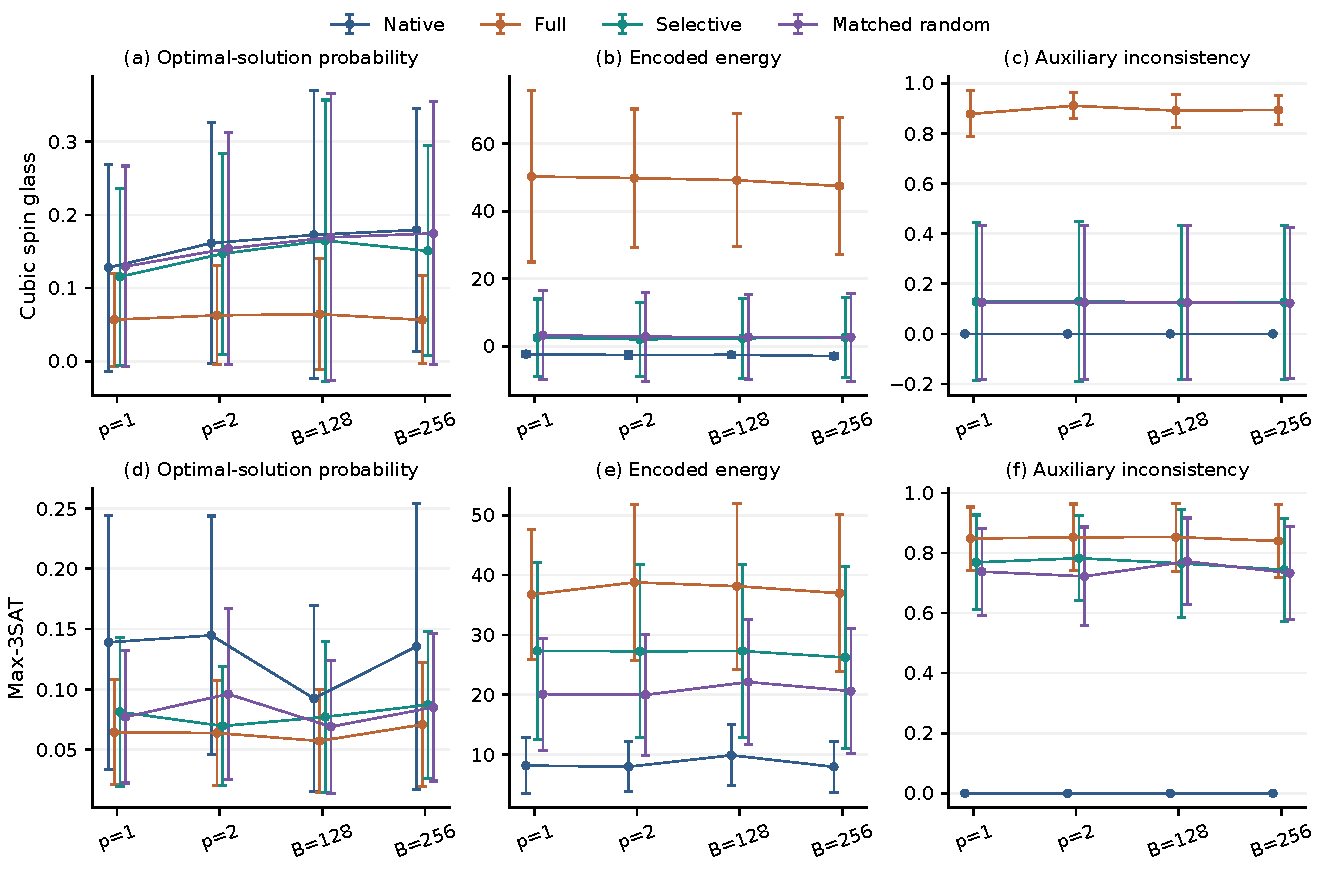
\includegraphics[width=\textwidth]{figures/figure_e3_secondary_metrics.pdf}
    \caption{Additional noiseless-QAOA diagnostics recalculated from the frozen
    run rows. Panels (a)--(c) show spin-glass optimal-solution probability,
    encoded energy, and auxiliary inconsistency $R_{\mathrm{inc}}$;
    (d)--(f) show the same metrics
    for Max-3SAT.  Restarts and matched-random draws are averaged before the raw
    instance is used as the statistical unit.  Encoded energy is
    representation-specific and is shown only as a diagnostic.}
    \label{fig:e3-secondary-metrics}
\end{figure}
The encoded energies should not be compared as a performance ranking because
the four representations use different encoded Hamiltonians.  The stored field
\nolinkurl{auxiliary_inconsistency_rate} implements the event in
\cref{eq:rinc}: it is the probability mass, or sampled fraction, for which at
least one active auxiliary relation is violated.  It is therefore exactly
$1-P_{\mathrm{cons}}$ for the active auxiliary set.


\FloatBarrier
\subsection{Original and targeted warm-start diagnostics}
\label{app:results-warmstart}

The stored first-stage sparse-RLT solver status was optimal for all 14 QAOA
test-labelled instances.  The returned vector contained 96 original-variable
pseudo-moments and 292 pair pseudo-moments, giving 388 diagnostic values in
total.  The selector-repaired schedule contains 62 distinct instance--representation/draw groups with active auxiliary variables, for which
the clipped pair pseudo-moments provide the auxiliary warm-start probabilities.

\Cref{fig:e4-signal-diagnostics} compares original-variable bias with pair
information. The pair pseudo-moments can differ from the independence closure;
this diagnostic alone does not establish a performance benefit.

\begin{figure}[!htbp]
    \centering
    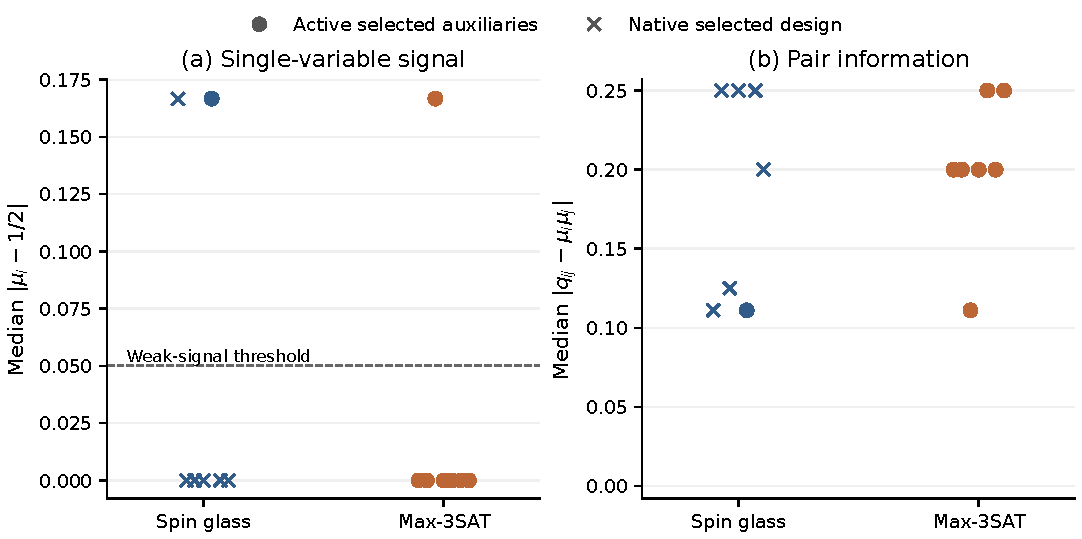
\includegraphics[width=\textwidth]{figures/figure_e4_signal_diagnostics.pdf}
    \caption{Signal available to the E4 warm start.  Each point summarises one
    raw QAOA instance.  Circles identify cases where the repaired selected
    representation has active auxiliaries; crosses identify a native selected
    endpoint. The LP values are unchanged; design-status markers are updated.
    Eleven of fourteen instances have weak single-variable signal. Two
    instances combine stronger signal with an active selected auxiliary design.}
    \label{fig:e4-signal-diagnostics}
\end{figure}

Only three instances exceed the weak-signal threshold, and two belong to
the eight-case common selective active-auxiliary subset.
\Cref{tab:e4-warmstart-common} reports the corrected outcomes on this fixed
subset, after averaging three restarts per instance and keeping each budget
separate. Before the selector repair, the coordinate-corrected original E4 schedule
contained 4,320 rows.
Positive-depth, zero-depth, and all-scheduled summaries for the full design
set are separately available in the correction archive. The selector-repaired
merged schedule retains 4,176 rows after 144 redundant warm-policy rows for
newly zero-auxiliary designs are removed.

\begin{table}[!htbp]
\centering\footnotesize
\setlength{\tabcolsep}{3pt}
\caption{Coordinate-corrected original E4 results on the frozen common selective active-auxiliary subset. Cold is the mean original objective; other columns are paired differences from cold with exploratory, unadjusted 95\% Student-$t$ intervals across $n$ raw instances. $n_0$ counts zero-layer instances retained in the scheduled comparison. Negative differences favour warm starts. Pair uses archived clipped pair moments; Ind. multiplies clipped original probabilities without further clipping.}
\label{tab:e4-warmstart-common}
\resizebox{\textwidth}{!}{%
\begin{tabular}{@{}lrrrlll@{}}
\toprule
Budget & $n$ & $n_0$ & Cold & Original-only minus cold & Pair minus cold & Ind. minus cold\\
\midrule
\multicolumn{7}{l}{\textbf{Spin glass}}\\
$p=1$ & 1 & 0 & $-1.093$ & $-0.715$ & $-0.647$ & $-0.681$\\
$p=2$ & 1 & 0 & $-1.722$ & $0.735$ & $-0.104$ & $0.164$\\
$B=128$ & 1 & 1 & $0.000$ & $-0.444$ & $-0.444$ & $-0.444$\\
$B=256$ & 1 & 0 & $-1.215$ & $0.290$ & $0.225$ & $0.307$\\
\addlinespace
\multicolumn{7}{l}{\textbf{Max-3SAT}}\\
$p=1$ & 7 & 0 & $10.035$ & $-0.562\;[-1.763,0.640]$ & $-0.872\;[-2.009,0.265]$ & $-0.552\;[-1.872,0.768]$\\
$p=2$ & 7 & 0 & $9.872$ & $-0.562\;[-1.741,0.616]$ & $-0.873\;[-2.154,0.408]$ & $-0.824\;[-2.036,0.387]$\\
$B=128$ & 7 & 2 & $9.884$ & $-0.647\;[-1.935,0.641]$ & $-0.677\;[-1.967,0.614]$ & $-0.808\;[-2.083,0.467]$\\
$B=256$ & 7 & 0 & $9.437$ & $-0.582\;[-1.795,0.632]$ & $-0.622\;[-1.879,0.635]$ & $-0.457\;[-2.034,1.121]$\\
\addlinespace
\bottomrule
\end{tabular}}
\end{table}

Spin-glass intervals are not estimable at $n=1$; all four Max-3SAT primary
pair-minus-cold intervals include zero. In the direct
pair-versus-original-only comparison, the Max-3SAT $p=2$ contrast is
$-0.311\;[-0.556,-0.065]$; the other such intervals and every
pair-versus-independence interval include zero. This secondary exploratory
contrast does not establish the primary pair-versus-cold claim.

\begin{figure}[!htbp]
\centering
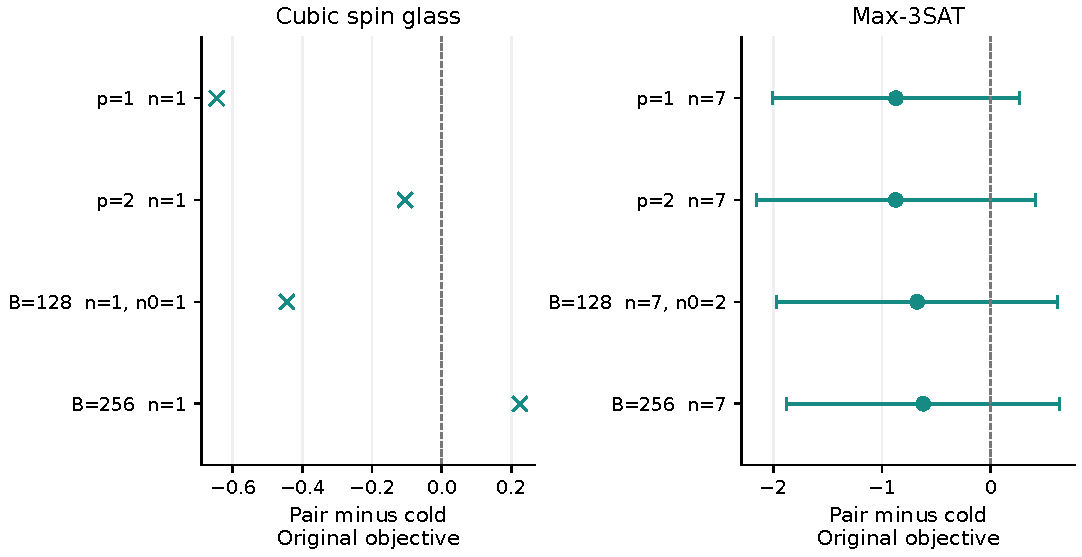
\includegraphics[width=\textwidth]{figures/figure_original_e4_warmstart_corrected.pdf}
\caption{Corrected original E4 pair-minus-cold differences on the selected
active-auxiliary subset. Error bars are exploratory instance-level 95\%
Student-$t$ intervals where estimable. The $n_0$ annotations identify retained
zero-layer instances; spin-glass crosses have $n=1$ and therefore no interval.}
\label{fig:e4-warmstart-corrected}
\end{figure}

\FloatBarrier
The targeted diagnostics and corrected warm-minus-cold plots below
complement \cref{tab:e4-strong-bias-warmstart}. The original screening
preceded QAOA evaluation; seven spin-glass and all ten Max-3SAT instances
exceed the signal threshold. Corrected mean optimal-solution probabilities
for targeted Max-3SAT under independence are $0.6094$ and $0.6224$ at
$p=1,2$, compared with $0.5987$ and $0.6262$ under pair warming.

\begin{figure}[!htbp]
    \centering
    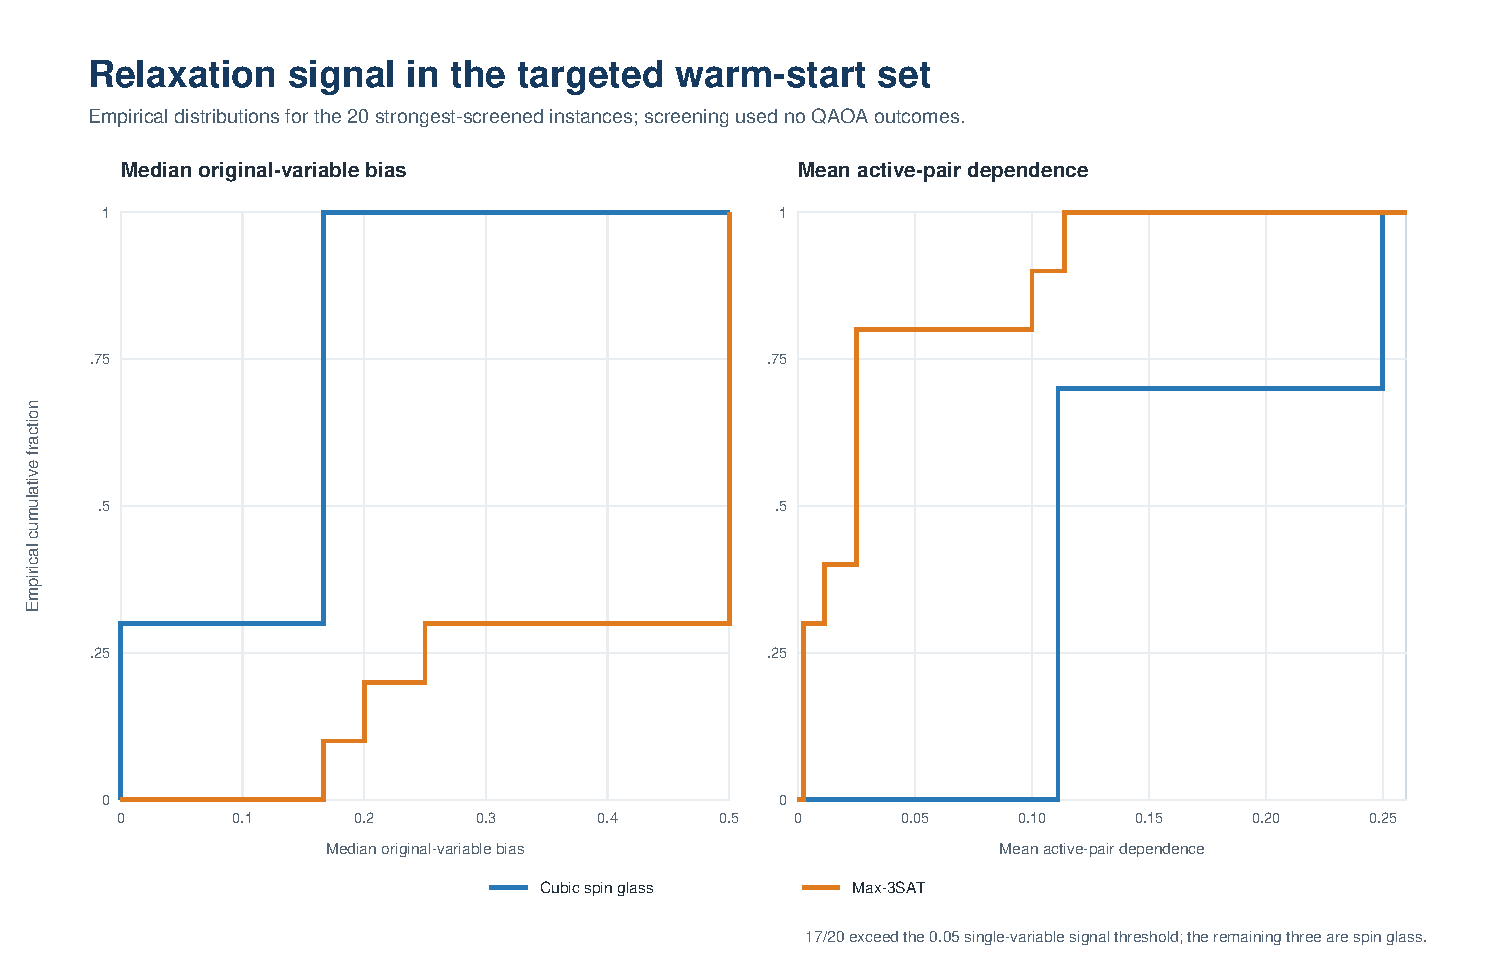
\includegraphics[width=\textwidth]
    {figures/figure_strong_bias_marginals.pdf}
    \caption{Relaxation-signal diagnostics for the 20 strongest-screened
    instances: (a) original-variable bias and (b) pair dependence.  Screening used only relaxation quantities and was completed
    before any QAOA outcome was inspected.  Seven spin-glass and all ten
    Max-3SAT instances exceed the frozen single-variable signal threshold.}
    \label{fig:e4-strong-bias-marginals}
\end{figure}


\begin{figure}[!htbp]
\centering
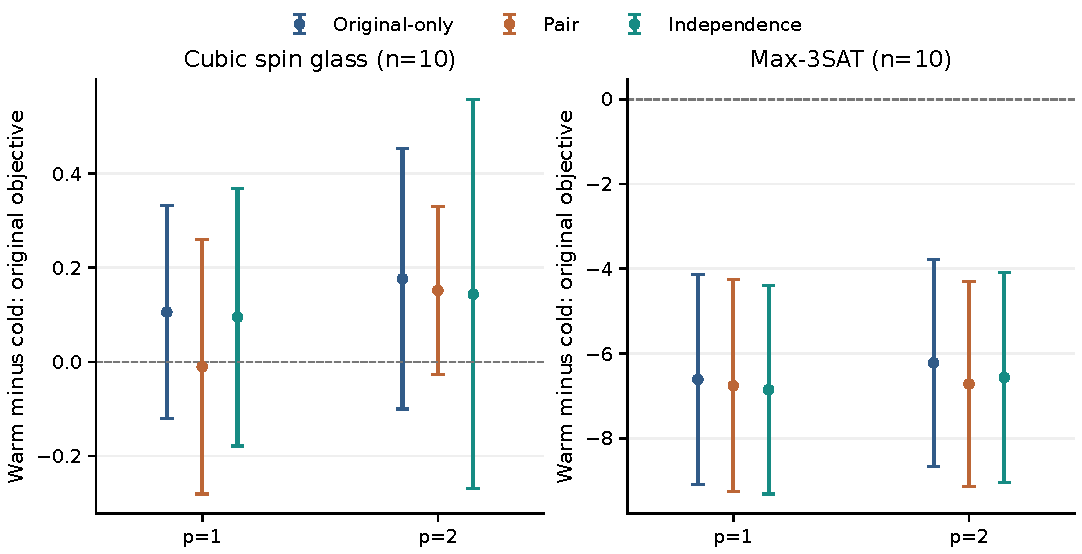
\includegraphics[width=\textwidth]{figures/figure_strong_bias_warmstart.pdf}
\caption{Coordinate-corrected mean paired warm-minus-cold original-objective
differences on the fixed strongest-screened set: (a) spin glass and
(b) Max-3SAT. The three policies are shown separately. Error bars are
exploratory, unadjusted 95\% Student-$t$ intervals over ten raw instances per
family after averaging three restarts. Negative differences favour warm starts.}
\label{fig:e4-strong-bias-warmstart}
\end{figure}

\FloatBarrier

\subsection{Complete descriptive regime counts}
\label{app:results-regimes}

We next compared selective reduction with its auxiliary-count-matched random
control.  The planned endpoints were two-qubit depth, two-qubit gate count,
routing overhead, and QAOA objective.  Outcomes not meeting either directional interval criterion were assigned
to the residual (inconclusive) category; this does not establish equivalence.

\begin{table}[!htbp]
    \centering
    \small
    \caption{Help, residual (inconclusive), hurt and not-estimable counts for
    selective reduction relative to the matched-random control. The residual
    category includes uncertain intervals and does not establish equivalence.}
    \label{tab:e5-regime-summary}
    \begin{tabular}{@{}llrrrr@{}}
        \toprule
        Family & Endpoint & Help & Residual & Hurt & Not estimable\\
        \midrule
        Cubic spin glass & Two-qubit depth  & 8 & 17 & 0 & 11\\
        Cubic spin glass & Two-qubit gates  & 3 & 22 & 0 & 11\\
        Cubic spin glass & Routing overhead & 1 & 24 & 0 & 11\\
        Cubic spin glass & QAOA objective   & 1 & 25 & 2 & 0\\
        \addlinespace
        Max-3SAT & Two-qubit depth  & 20 & 0 & 0 & 16\\
        Max-3SAT & Two-qubit gates  & 19 & 1 & 0 & 16\\
        Max-3SAT & Routing overhead & 1 & 19 & 0 & 16\\
        Max-3SAT & QAOA objective   & 1 & 13 & 14 & 0\\
        \bottomrule
    \end{tabular}
\end{table}

Of 272 scheduled instance--metric endpoints, 191 were estimable: 54 helped,
121 were classified as residual (inconclusive) and 16 hurt; 81 were not estimable. In the

QAOA rows, each family contributes seven instances at four budgets.
Thirty-nine residual intervals extend beyond the tolerance band.
Classification follows
Appendix~\ref{app:experimental-statistics}; these are endpoint counts,
not independent-instance confidence statements.

The 81 not-estimable endpoints were expected sparse-device infeasibilities.
All-to-all data were estimable for all 18 instances in each family, while the
sparse-topology data were estimable for only seven of 18 spin-glass instances
and two of 18 Max-3SAT instances.  Some sparsity and pair-reuse bins also
contain only one or two observations.  The regime counts therefore show useful
patterns, but they are too small for a universal rule about problem structure.

\FloatBarrier
\subsection{Limited study with a representative noise model}
\label{sec:results-noise}

The 18-instance noise study follows the fixed simulator configuration in
Appendix~\ref{app:noise-protocol}. The tables below report absolute objectives,
degradation from each representation's own sampled noiseless baseline, and
paired selective-minus-native differences.

\begin{table}[!htbp]
    \centering
    \small
    \caption{Descriptive means in the limited noise study.  Lower objective
    values are better.  Degradation is the high-noise objective minus the
    noiseless objective.  The final column is the high-noise auxiliary
    inconsistency rate $R_{\mathrm{inc}}$ from \cref{eq:rinc}.}
    \label{tab:e6-noise-summary}
    \resizebox{\linewidth}{!}{%
\begin{tabular}{@{}llrrrrr@{}}
        \toprule
        Family & Representation
        & Noiseless & Low noise & High noise
        & Degradation & Inconsistency\\
        \midrule
        Cubic spin glass
        & Native          & -3.052 & -0.699 & -0.087 & 2.965 & 0.000\\
        & Fully reduced   & -0.620 & -0.175 & -0.032 & 0.588 & 0.872\\
        & Selective       & -2.923 & -0.729 & -0.123 & 2.800 & 0.083\\
        & Matched random  & -2.953 & -0.769 & -0.124 & 2.829 & 0.082\\
        \addlinespace
        Max-3SAT
        & Native          & 7.953 & 9.305 & 9.700 & 1.748 & 0.000\\
        & Fully reduced   & 9.024 & 9.396 & 9.633 & 0.609 & 0.821\\
        & Selective       & 8.701 & 9.455 & 9.692 & 0.990 & 0.775\\
        & Matched random  & 8.402 & 9.302 & 9.642 & 1.239 & 0.771\\
        \bottomrule
    \end{tabular}}%

\end{table}

Noise worsened every representation's mean original objective. Full reduction
changed least from its noiseless value, but started worse than native in both
families and retained high auxiliary inconsistency. Selective reduction had
lower inconsistency than full reduction for spin glass, but remained highly
inconsistent for Max-3SAT. Smaller degradation is not better absolute performance.

This table is descriptive.  The raw file contains three repeated rows per
instance for the native, fully reduced, and selective representations, and 15
rows for the five matched-random designs.  These repeated rows were therefore
averaged inside each raw instance before any uncertainty calculation.

\begin{table}[!htbp]
    \centering
    \small
    \caption{Instance-level selective-minus-native objective differences in
    the noise study.  Lower objective values are better, so a negative mean
    favours selective reduction.  The 95\% intervals are Student-$t$
    intervals across nine raw instances per family.  W/T/L gives the numbers
    of instance wins, ties, and losses using the predeclared 0.01 objective
    equivalence band.}
    \label{tab:e6-paired-noise}
    \begin{tabular}{@{}llrrrl@{}}
        \toprule
        Family & Noise & Mean difference & 95\% interval & $d_z$ & W/T/L\\
        \midrule
        Cubic spin glass & Noiseless & $0.129$  & $[-0.868,1.126]$ & $0.099$  & 5/0/4\\
                          & Low       & $-0.030$ & $[-0.312,0.251]$ & $-0.083$ & 6/0/3\\
                          & High      & $-0.036$ & $[-0.089,0.016]$ & $-0.532$ & 4/3/2\\
        \addlinespace
        Max-3SAT         & Noiseless & $0.749$  & $[0.140,1.358]$  & $0.945$  & 3/0/6\\
                          & Low       & $0.149$  & $[-0.046,0.344]$ & $0.589$  & 1/0/8\\
                          & High      & $-0.009$ & $[-0.133,0.116]$ & $-0.053$ & 5/0/4\\
        \bottomrule
    \end{tabular}
\end{table}

After within-instance aggregation, neither non-zero noise level showed a
clear selective advantage over native. All spin-glass intervals included zero;
Max-3SAT favoured native without noise and was inconclusive under noise.
The smaller Max-3SAT degradation starts from a worse noiseless baseline and
does not establish better absolute noisy performance. With nine instances
per family, this is an exploratory robustness check.

\end{document}

